%% =====================================================================
%%  LUẬN VĂN THẠC SĨ — Lê Đoàn Phương Uyên
%%  "Sinh hướng dẫn sử dụng phần mềm từ ảnh màn hình"
%%  Biên dịch:  tectonic main.tex        (hoặc  ./build.sh)
%%
%%  ⚠️ Ô CẦN ĐIỀN / KIỂM LẠI trước khi in — xem README.md mục 3.
%% =====================================================================
\documentclass[12pt,a4paper,oneside]{report}
% Cỡ chữ 13pt (chuẩn luận văn tiếng Việt). Nếu môi trường không có gói `fontsize`,
% xoá dòng \usepackage[...]{fontsize} bên dưới thì tài liệu về 12pt và vẫn biên dịch được.
\usepackage[fontsize=13pt]{fontsize}

% ---- thông tin thay đổi được, sửa ở đây thay vì sửa trong thân bài ----
\newcommand{\TenDeTai}{Sinh hướng dẫn sử dụng phần mềm\\từ ảnh màn hình}
\newcommand{\TenDeTaiMotDong}{Sinh hướng dẫn sử dụng phần mềm từ ảnh màn hình}
\newcommand{\TenDeTaiEN}{Generating Software Usage Instructions from Screenshots}
\newcommand{\HocVien}{Lê Đoàn Phương Uyên}
\newcommand{\MSHV}{24C15039}                      % ⚠️ KIỂM LẠI
\newcommand{\GVHD}{TS. Nguyễn Hồng Bửu Long}
\newcommand{\GVHDen}{Dr. Nguyen Hong Buu Long}
\newcommand{\Nganh}{Trí tuệ nhân tạo}
\newcommand{\MaNganh}{8480107}
% Khoá 34 (user xác nhận 30/8/2026); MSHV 24C15039 = nhập học 2024.
\newcommand{\Khoa}{34}
\newcommand{\NamBaoVe}{2026}
\newcommand{\NgayHoanThanh}{Tp. Hồ Chí Minh, tháng 8 năm 2026}

% ---- font: dùng đúng bộ đã kiểm chạy được với tectonic trong repo này ----
\usepackage{fontspec}
\setmainfont{texgyretermes}[
  Extension = .otf, UprightFont = *-regular, BoldFont = *-bold,
  ItalicFont = *-italic, BoldItalicFont = *-bolditalic ]
\setsansfont{texgyreheros}[
  Extension = .otf, UprightFont = *-regular, BoldFont = *-bold,
  ItalicFont = *-italic, BoldItalicFont = *-bolditalic ]
\setmonofont{texgyrecursor}[
  Extension = .otf, UprightFont = *-regular, BoldFont = *-bold,
  ItalicFont = *-italic, BoldItalicFont = *-bolditalic, Scale = MatchLowercase ]

\usepackage{amsmath,amssymb}
\usepackage{unicode-math}
\setmathfont{texgyretermes-math.otf}
\usepackage{graphicx}
\usepackage{booktabs}
\usepackage{array}
\usepackage{longtable}
\usepackage{multirow}
\usepackage{enumitem}
\usepackage{setspace}
\usepackage[table]{xcolor}
\usepackage{caption}
\usepackage{url}
\usepackage[hidelinks]{hyperref}
\usepackage[left=3.5cm,right=2cm,top=2.5cm,bottom=2.5cm]{geometry}
\usepackage{fancyhdr}
\usepackage{titlesec}
\usepackage{tabularx}
\usepackage{tikz}
\usetikzlibrary{positioning,arrows.meta,backgrounds,fit}

\onehalfspacing
\setlength{\parskip}{0.35em}
% Tiếng Việt không có bộ luật ngắt âm tiết trong TeX nên các dòng dài dễ tràn lề.
% emergencystretch cho phép giãn khoảng trắng ở dòng cuối cùng thay vì đẩy chữ ra lề.
\emergencystretch=3.5em
\captionsetup{font=small,labelfont=bf}

% ---- Việt hoá tên mục tự sinh (không dùng gói ngôn ngữ để tránh phụ thuộc) ----
\renewcommand{\contentsname}{Mục lục}
\renewcommand{\listfigurename}{Danh mục các hình vẽ, đồ thị}
\renewcommand{\listtablename}{Danh mục các bảng số liệu}
\renewcommand{\bibname}{Tài liệu tham khảo}
\renewcommand{\chaptername}{Chương}
\renewcommand{\figurename}{Hình}
\renewcommand{\tablename}{Bảng}
\renewcommand{\appendixname}{Phụ lục}

\titleformat{\chapter}[display]
  {\normalfont\huge\bfseries}{\chaptertitlename\ \thechapter}{18pt}{\Huge}
\titlespacing*{\chapter}{0pt}{0pt}{28pt}

\pagestyle{fancy}
\fancyhf{}
\fancyfoot[C]{\thepage}
\renewcommand{\headrulewidth}{0pt}

% ---- ký hiệu dùng nhiều lần ----
\newcommand{\pp}{\,pp}                    % percentage point
\newcommand{\ktc}[2]{[#1;\,#2]}
\newcommand{\code}[1]{\texttt{\small #1}}
\newcommand{\CANDIEN}[1]{\textcolor{red}{\textbf{[CẦN ĐIỀN: #1]}}}
\newcommand{\CHOSO}[1]{\textcolor{red}{\textbf{[CHỜ SỐ: #1]}}}

\begin{document}

% Hai trang bìa KHÔNG được đánh số và không tính vào số trang La Mã.
% ===================== BÌA NGOÀI =====================
\thispagestyle{empty}
\begin{center}

{\large ĐẠI HỌC QUỐC GIA TP. HỒ CHÍ MINH}\\[0.3em]
{\large TRƯỜNG ĐẠI HỌC KHOA HỌC TỰ NHIÊN}\\[6em]

{\Large \HocVien}\\[5em]

{\LARGE\bfseries \MakeUppercase{\TenDeTai}}\\[6em]

{\Large\bfseries LUẬN VĂN THẠC SĨ}\\[8em]

{\large TP. Hồ Chí Minh - Năm \NamBaoVe}

\end{center}
\clearpage

% ===================== BÌA TRONG =====================
\thispagestyle{empty}
\begin{center}

{\large ĐẠI HỌC QUỐC GIA TP. HỒ CHÍ MINH}\\[0.3em]
{\large TRƯỜNG ĐẠI HỌC KHOA HỌC TỰ NHIÊN}\\[4.5em]

{\Large \HocVien}\\[4em]

{\LARGE\bfseries \MakeUppercase{\TenDeTai}}\\[4em]

{\large Ngành: \MakeUppercase{\Nganh}}\\[0.4em]
{\large Mã số ngành: \MaNganh}\\[4em]

{\large\bfseries NGƯỜI HƯỚNG DẪN KHOA HỌC}\\[0.4em]
{\large \GVHD}\\[6em]

{\large TP. Hồ Chí Minh - Năm \NamBaoVe}

\end{center}
\clearpage


% Đánh số La Mã bắt đầu từ Lời cam đoan = i (đúng quy cách luận văn).
\pagenumbering{roman}
% ===================== LỜI CAM ĐOAN =====================
\chapter*{Lời cam đoan}
\addcontentsline{toc}{chapter}{Lời cam đoan}

Tôi cam đoan luận văn thạc sĩ ngành \Nganh{} với đề tài \textbf{\TenDeTaiMotDong}
là công trình do tôi thực hiện dưới sự hướng dẫn của \GVHD.

Các số liệu và kết quả trình bày trong luận văn là trung thực, được tính từ mã nguồn cùng
các tệp kết quả đi kèm, và chưa từng được công bố trong công trình của tác giả khác. Những
thí nghiệm đã lên kế hoạch nhưng chưa thực hiện đều được ghi rõ là chưa thực hiện. Các tài liệu
tham khảo được trích dẫn đầy đủ.

Tôi xin chịu trách nhiệm về tính trung thực của các kết quả trình bày trong luận văn.

\vspace{2em}
\begin{flushright}
\begin{minipage}{0.42\textwidth}
\centering
Học viên cao học\\[4em]
\HocVien
\end{minipage}
\end{flushright}
\clearpage

% ===================== LỜI CẢM ƠN =====================
\chapter*{Lời cảm ơn}
\addcontentsline{toc}{chapter}{Lời cảm ơn}

Luận văn được hoàn thành tại Khoa Công nghệ Thông tin, Trường Đại học Khoa học Tự nhiên,
Đại học Quốc gia Thành phố Hồ Chí Minh, dưới sự hướng dẫn của \GVHD.

Trước hết, tôi xin gửi lời cảm ơn chân thành đến thầy hướng dẫn, người đã định hướng đề
tài và góp ý cho tôi trong suốt quá trình thực hiện luận văn.

Tôi xin cảm ơn quý thầy cô Khoa Công nghệ Thông tin đã giảng dạy trong suốt chương trình
cao học, và cảm ơn Văn phòng Khoa đã hỗ trợ các thủ tục liên quan đến luận văn.

Cuối cùng, tôi xin cảm ơn gia đình đã tạo điều kiện để tôi theo học và hoàn thành
chương trình này.

\vspace{2em}
\begin{flushright}
\begin{minipage}{0.42\textwidth}
\centering
\NgayHoanThanh\\[4em]
\HocVien
\end{minipage}
\end{flushright}
\clearpage


\tableofcontents
\cleardoublepage
\addcontentsline{toc}{chapter}{Danh mục các hình vẽ, đồ thị}
\listoffigures
\cleardoublepage
\addcontentsline{toc}{chapter}{Danh mục các bảng số liệu}
\listoftables

\chapter*{Danh mục các từ viết tắt, khái niệm và thuật ngữ}
\addcontentsline{toc}{chapter}{Danh mục các từ viết tắt, khái niệm và thuật ngữ}

\renewcommand{\arraystretch}{1.35}
\begin{longtable}{@{}p{2.6cm}p{5.4cm}p{6.2cm}@{}}
\toprule
\textbf{Viết tắt} & \textbf{Từ đầy đủ} & \textbf{Tiếng Việt / giải thích} \\
\midrule
\endfirsthead
\toprule
\textbf{Viết tắt} & \textbf{Từ đầy đủ} & \textbf{Tiếng Việt / giải thích} \\
\midrule
\endhead

GUI & Graphical User Interface & Giao diện đồ hoạ người dùng \\
VLM & Vision-Language Model & Mô hình thị giác và ngôn ngữ \\
LLM & Large Language Model & Mô hình ngôn ngữ lớn \\
SFT & Supervised Fine-Tuning & Tinh chỉnh có giám sát \\
LoRA & Low-Rank Adaptation & Tinh chỉnh hạng thấp \\
QLoRA & Quantized LoRA & LoRA trên trọng số đã lượng tử hoá \\
NF4 & 4-bit NormalFloat & Định dạng lượng tử hoá 4 bit \\
AC & AndroidControl & Bộ dữ liệu điều khiển Android (NeurIPS 2024) \\
AITW & AndroidInTheWild & Bộ dữ liệu Android quy mô lớn (NeurIPS 2023) \\
OCR & Optical Character Recognition & Nhận dạng chữ trong ảnh \\
VH & View Hierarchy & Cây phân cấp khung nhìn của màn hình Android \\
a11y & Accessibility (tree) & Cây trợ năng; nguồn khai báo vai trò và tên phần tử \\
REG & Referring Expression Generation & Sinh biểu thức quy chiếu (mô tả phân biệt một đối tượng) \\
MDE & Minimum Detectable Effect & Mức chênh lệch nhỏ nhất còn phân biệt được với nhiễu \\
KTC & (Confidence Interval) & Khoảng tin cậy \\
dp & density-independent pixel & Đơn vị độ dài độc lập mật độ điểm ảnh trên Android \\
pp & percentage point & Điểm phần trăm (chênh lệch tuyệt đối giữa hai tỉ lệ) \\
ORPO & Odds Ratio Preference Optimization & Mục tiêu ưu tiên gắn thẳng vào hàm mất mát có
giám sát, không cần mô hình tham chiếu \\
\midrule
\multicolumn{3}{@{}l@{}}{\textit{Thuật ngữ riêng của luận văn}} \\
\midrule
\multicolumn{2}{@{}p{8.2cm}}{\textit{executability} (tính thực thi được)}
& Thước đo mà luận văn đề xuất. Một câu hướng dẫn được tính là đúng nếu đưa câu đó cho
một mô hình định vị độc lập thì nó chỉ trúng phần tử mà người dùng đã chạm \\
\multicolumn{2}{@{}p{8.2cm}}{Mô hình định vị phần tử (\textit{GUI grounding model})}
& Mô hình nhận một câu mô tả cùng một ảnh màn hình và trả về toạ độ của phần tử được mô
tả. Ở đây nó đóng vai \textbf{dụng cụ đo}, không phải một hệ thống đem ra so sánh \\
\multicolumn{2}{@{}p{8.2cm}}{Dòng khai báo (\textit{descriptor})}
& Một dòng có cấu trúc gồm bốn ô, \code{[vai trò | tên | toạ độ | dấu hiệu phân biệt]},
mà mô hình phải viết ra trước khi viết câu hướng dẫn. Dòng này bị cắt bỏ trước khi chấm \\
\multicolumn{2}{@{}p{8.2cm}}{Ô Voronoi}
& Vùng trên màn hình gồm những điểm nằm gần phần tử cần chạm hơn bất kỳ phần tử nào khác.
Luận văn dùng vùng này để xác định thế nào là trỏ trúng, thay cho một ngưỡng sai số cố
định \\
\multicolumn{2}{@{}p{8.2cm}}{Bước chạm}
& Bước thao tác mà người dùng chạm vào màn hình, tức bước có toạ độ đích. Toàn bộ điểm số
của luận văn tính trên nhóm bước này \\
\multicolumn{2}{@{}p{8.2cm}}{Phần tử cần chạm}
& Nút, ô nhập hoặc mục danh sách mà người dùng đã chạm ở bước đang xét, tức thứ mà câu
hướng dẫn phải chỉ ra được \\
\multicolumn{2}{@{}p{8.2cm}}{Quần thể chấm}
& Tập $4.463$ bước chạm của tập kiểm, dùng chung cho mọi nhánh, nên hai nhánh bất kỳ luôn
so được với nhau trên cùng những bước \\
\multicolumn{2}{@{}p{8.2cm}}{Trần và sàn của thước}
& Trần là điểm mà câu do người viết đạt được, tức mức cao nhất mà thước còn cho. Sàn là
điểm mà một câu không mang thông tin gì vẫn đạt được. Mọi điểm số đọc trong dải giữa hai
mức đó \\
\multicolumn{2}{@{}p{8.2cm}}{Nhánh nền và nhánh xử lý}
& Nhánh nền là nhánh không có thành phần đề xuất, dùng làm mốc so. Nhánh xử lý là nhánh
có thành phần đó. Chênh lệch giữa hai nhánh chính là đại lượng cần đo \\
\multicolumn{2}{@{}p{8.2cm}}{Hạt giống}
& Số dùng để khởi tạo phần ngẫu nhiên của một lượt huấn luyện. Hai lượt chỉ khác hạt
giống là hai lần dựng lại cùng một hệ thống, nên chênh lệch giữa chúng là nhiễu \\
\multicolumn{2}{@{}p{8.2cm}}{Điểm lưu (\textit{checkpoint})}
& Bản trọng số mô hình được ghi ra đĩa tại một thời điểm của lượt huấn luyện \\
\multicolumn{2}{@{}p{8.2cm}}{Lát cắt}
& Một cách chia quần thể chấm thành các nhóm nhỏ để đọc kết quả riêng trên từng nhóm, ví
dụ chia theo độ dài câu hoặc theo số phần tử trên màn hình \\
\multicolumn{2}{@{}p{8.2cm}}{Phép so đối chiếu}
& Một chênh lệch đã biết chắc dấu và đủ lớn, dùng để kiểm xem một cách đo mới có còn nhìn
thấy những khác biệt thật hay không \\
\multicolumn{2}{@{}p{8.2cm}}{MIN-DESC}
& Chặng huấn luyện thứ hai, nối tiếp nhánh S2. Mô hình học từ những cặp câu chỉ khác nhau
ở dòng khai báo, còn phần câu hướng dẫn thì giống hệt nhau (Mục~\ref{sec:mindescthietke}) \\
\multicolumn{2}{@{}p{8.2cm}}{CE2-S2}
& Nhánh đối chứng của MIN-DESC, dùng để tách xem phần cải thiện nào là của mục tiêu huấn
luyện mới và phần nào chỉ do được học thêm \\
\bottomrule
\end{longtable}
\clearpage

\chapter*{Trang thông tin luận văn}
\addcontentsline{toc}{chapter}{Trang thông tin luận văn tiếng Việt}
\begin{center}\textbf{\large TRANG THÔNG TIN LUẬN VĂN}\end{center}

\renewcommand{\arraystretch}{1.25}
\noindent\begin{tabularx}{\textwidth}{@{}lX@{}}
Tên đề tài luận văn: & \TenDeTaiMotDong. \\
Ngành: & \Nganh \\
Mã số ngành: & \MaNganh \\
Họ và tên HVCH: & \HocVien \\
Khóa đào tạo: & \Khoa \\
GVHD: & \GVHD \\
Cơ sở đào tạo: & Trường ĐH Khoa học Tự nhiên, ĐHQG-HCM \\
\end{tabularx}

\subsection*{1. Tóm tắt nội dung luận văn}

Các mô hình giao diện hiện nay sinh ra toạ độ để máy tự bấm. Luận văn nghiên cứu một
đầu ra khác trên cùng dữ liệu vào: một câu tiếng Anh nói cho \emph{người đọc} biết phải
chạm vào phần tử nào trên màn hình. Trở ngại chính không nằm ở khâu sinh câu mà ở khâu
chấm: cùng một nút có nhiều cách gọi tên hợp lệ, nên không câu chuẩn đơn lẻ nào gánh
được vai trò đáp án.

Luận văn đề xuất thước đo \textbf{executability}: câu sinh ra được đưa cho một mô hình
định vị phần tử độc lập, mô hình này không hề thấy toạ độ đáp án; bước được tính đúng
khi điểm nó trả về rơi vào ô Voronoi của phần tử người dùng đã chạm và loại thao tác
được gọi tên đúng. Thước được kiểm bằng bốn phép độc lập trước khi dùng để kết luận:
một cổng chặn về sai số của dụng cụ đo (đạt: sai số trung vị $0{,}7\%$ bề ngang màn so
với ngưỡng $3\%$ khoá trước), một phép chọn luật trúng dựa trên \emph{sàn} đo được (luật
dung sai quy ước cho điểm $84{,}3\%$ số câu chỉ sai nút, luật ô Voronoi chỉ $2{,}8\%$),
một phép đo trần ($75{,}7\%$, KTC 95\% $[74{,}1; 77{,}3]$ khi đưa chính câu người viết đi
chấm), và một bộ bơm lỗi với ngưỡng đóng băng trước khi chạy.

Về phía mô hình, luận văn xây dựng hoàn toàn tự động một tập giám sát $64.567$ bước từ
bộ AndroidControl, không thuê người dán nhãn, đã kiểm rò rỉ dạy--kiểm ở quy mô đủ và
không tìm thấy tác vụ nào trùng. Thành phần đề xuất là ``mô tả phân biệt trước, phát
ngôn sau'': đích huấn luyện chứa một dòng khai báo có cấu trúc về phần tử đích trước khi
tới câu, và dòng khai báo bị cắt bỏ trước khi chấm.

Trên $4.463$ bước chạm của tập kiểm, mô hình Qwen2.5-VL-3B tinh chỉnh QLoRA đạt
$59{,}1\%$ so với $47{,}6\%$ của chính mô hình đó khi chưa tinh chỉnh; chênh lệch ghép
cặp $11{,}5$ điểm ($p<0{,}001$) đứng vững qua năm cách giải thích thay thế, còn cách thứ
sáu (bắt chước văn phong) chưa loại trừ được.

\subsection*{2. Những kết quả mới của luận văn}

\begin{itemize}[leftmargin=1.4em]
\item \textbf{Thước đo không cần đáp án tham chiếu cho bài toán sinh hướng dẫn giao
diện.} Luật trúng được chọn dựa trên hành vi đo được với đầu vào sai nút, không dựa
trên ngưỡng dung sai quy ước; thứ tự giữa các hệ thống giữ nguyên dưới năm luật chấm
khác nhau.

\item \textbf{Trần của thước được đo, không phải giả định.} Đưa chính câu do người viết
đi chấm cho $75{,}7\%$; mọi điểm số của mô hình phải đọc trên nền này chứ không phải
trên nền $100$. Ước lượng cũ $70{,}0\%$ dựa trên mẫu con $300$ bước lệch $5{,}7$ điểm và
đã bị rút.

\item \textbf{Đường ống dữ liệu tự động.} Chuyển AndroidControl thành tập giám sát cho
tác vụ mới: ghép hai bản phân phối trên Hugging Face, kiểm phép ghép bằng đối chứng lệch
một bước ($48\%$ so với $20\%$), dựng nhãn mô tả từ cây trợ năng kết hợp OCR, chín bất
biến cấu trúc đều đạt ở quy mô đủ.

\item \textbf{Bản đăng ký trước có luật đọc cho cả bốn kết cục}, đưa vào kho phiên bản
trước lượt huấn luyện đầu tiên; mọi thay đổi về sau ghi thành mục sửa đổi có ngày.

\item \textbf{Định vị bài toán.} Trong bộ AndroidControl gốc và trong các công trình
dùng bộ này, câu hướng dẫn từng bước do người viết nằm ở \emph{đầu vào}; ở đây nó là
\emph{đích sinh} và là đầu ra duy nhất đem chấm.
\end{itemize}

\vspace{1.5em}
\noindent\begin{tabularx}{\textwidth}{@{}XX@{}}
\centering CÁN BỘ HƯỚNG DẪN & \centering\arraybackslash HỌC VIÊN CAO HỌC \\
\centering (Ký tên, họ tên) & \centering\arraybackslash (Ký tên, họ tên) \\
\end{tabularx}

\vspace{4em}
\begin{center}
XÁC NHẬN CỦA CƠ SỞ ĐÀO TẠO\\ HIỆU TRƯỞNG
\end{center}
\clearpage

% ==================== BẢN TIẾNG ANH ====================
\chapter*{Thesis information}
\addcontentsline{toc}{chapter}{Trang thông tin luận văn tiếng Anh}
\begin{center}\textbf{\large THESIS INFORMATION}\end{center}

\noindent\begin{tabularx}{\textwidth}{@{}lX@{}}
Thesis title: & \TenDeTaiEN. \\
Speciality: & Computer Science \\
Code: & \MaNganh \\
Name: & Le Doan Phuong Uyen \\
Academic year: & \Khoa \\
Supervisor: & \GVHDen \\
At: & VNUHCM -- University of Science \\
\end{tabularx}

\subsection*{1. Summary}

GUI agents produce coordinates for a machine to click. This thesis studies a different
output over the same input: a short instruction telling a \emph{person} which on-screen
element to touch. The obstacle is not generation but evaluation, since many wordings
identify the same button and no single reference can carry the judgement.

We propose \textbf{executability}: the generated sentence is passed to a separate GUI
grounding model that never sees the gold coordinate, and a step counts as correct when
the returned point falls in the Voronoi cell of the element the user touched and the
described action type matches. The instrument is characterised before it is trusted: an
adequacy gate on grounder error (passed, median 0.7\% of screen width against a
threshold of 3\% fixed in advance), a hit rule selected from its measured floor (the
conventional tolerance test credits a sentence naming the wrong button in 84.3\% of
cases, the cell rule in 2.8\%), a measured ceiling of 75.7\% (95\% CI
$[74.1, 77.3]$) obtained by scoring the human-written references themselves, and a
perturbation self-check with thresholds fixed before execution.

On the model side we build 64,567 supervision steps from AndroidControl fully
automatically, with zero task-level train--test leakage verified at full scale. The
proposed component is descriptor-first generation: the training target carries a
structured descriptor of the target element before the sentence, and the descriptor is
removed before scoring.

Over 4,463 held-out touch steps a QLoRA-tuned Qwen2.5-VL-3B reaches 59.1\% against
47.6\% for the same model untuned; the paired gap of 11.5 points ($p<0.001$)
survives five checks for alternative explanations; a sixth, imitation of the annotator
register, is not ruled out.

\subsection*{2. Novelty of thesis}

\begin{itemize}[leftmargin=1.4em]
\item A reference-free metric for element identification in generated GUI instructions,
with the hit rule selected from measured behaviour on wrong-element inputs rather than
from a tolerance convention, and shown to preserve system ordering under five different
rules.
\item A measured, not assumed, ceiling: human-written references score 75.7\%, the
level every model score must be read against. An earlier 70.0\% estimate from a
300-step subsample was five points low and has been retracted.
\item A fully automatic pipeline converting AndroidControl into supervision for this
task, with the cross-modal join validated against a deliberately shifted control
(48\% against 20\%).
\item A pre-registered ablation design fixing the reading of all four outcomes,
committed to version control before the first training run.
\item Positioning: in AndroidControl and in work built on it, the human-written
per-step instruction is an \emph{input}; here it is the generation target and the only
scored output.
\end{itemize}

\vspace{1.5em}
\noindent\begin{tabularx}{\textwidth}{@{}XX@{}}
\centering SUPERVISOR & \centering\arraybackslash MASTER STUDENT \\
\end{tabularx}

\vspace{4em}
\begin{center}
CERTIFICATION\\ UNIVERSITY OF SCIENCE\\ PRESIDENT
\end{center}
\clearpage


\clearpage
\pagenumbering{arabic}
\setcounter{page}{1}

\chapter{Giới thiệu}
\label{ch:gioithieu}

\section{Đặt vấn đề}

Khi thao tác trên điện thoại, người dùng nhiều lúc dừng lại giữa chừng vì không rõ bước
tiếp theo phải làm gì. Điều họ cần trong tình huống đó là một câu chỉ dẫn cho đúng bước
trước mắt, chẳng hạn ``Chạm vào biểu tượng chia sẻ ở góc trên bên phải màn hình''. Với dạng
câu hướng dẫn ngắn và chỉ nói về màn hình người dùng đang mở như vậy, đối tượng tiếp nhận
là con người chứ không phải phần mềm.

Dòng nghiên cứu về tác tử giao diện (\emph{GUI agent}) những năm gần đây giải một bài toán
rất gần với bài toán trên, nhưng khác hẳn ở bản chất của đầu ra. Cho cùng một ảnh màn hình và cùng một mục
tiêu, các hệ thống như SeeClick~\cite{seeclick}, OS-Atlas~\cite{osatlas} hay
Aguvis~\cite{aguvis} sinh ra một lệnh máy đọc được, dạng \code{click(872,141)}, để phần
mềm tự bấm thay người. Câu chữ, nếu có xuất hiện, chỉ là biểu diễn trung gian dẫn tới lệnh đó và không được đem chấm.

Luận văn nhận cùng đầu vào đó, nhưng lấy câu chữ làm sản phẩm cuối cùng. Đầu ra là một
câu hướng dẫn cho người đọc, và đó cũng là thứ duy nhất được đem đánh giá. Việc đổi đầu ra
như vậy kéo theo hai vấn đề chưa có lời giải sẵn.

\textbf{Vấn đề thứ nhất là đánh giá.} Một toạ độ dự đoán có thể đem so trực tiếp với toạ
độ mà người dùng đã chạm. Một câu thì không so được với một câu chuẩn duy nhất, bởi cùng
một nút thường có nhiều cách gọi tên đều đúng. Chẳng hạn ``Click on the search bar'' và
``Tap the magnifying glass at the top'' cùng chỉ một phần tử, và không bộ dữ liệu nào liệt kê hết
các cách diễn đạt hợp lệ.

Các thước đo quen dùng đều thất bại ở đúng điểm này, và luận văn đo mức thất bại của từng
thước. So khớp chuỗi ký tự loại nhầm $97{,}5\%$ số câu diễn đạt khác. So vector ngữ nghĩa cho
diện tích dưới đường ROC (AUC) chỉ $0{,}336$ trên $51$ trường hợp viết tay, tức còn kém hơn
đoán ngẫu nhiên. Lý do là vector ngữ nghĩa đo độ gần về \emph{chủ đề}, trong khi thứ cần
đo lại là hai câu có nói về \emph{cùng một phần tử} hay không. Ở phép thử này, cặp
\code{inbox} và \code{outbox} được chấm $0{,}76$, cao hơn hẳn cặp \code{search} và \code{magnifying
glass} chỉ được $0{,}55$, dù cặp sau mới là cặp cùng chỉ một nút. Chi tiết ở
Mục~\ref{sec:thuoc-gay}.

\textbf{Vấn đề thứ hai nằm ở dạng lỗi mà mô hình sinh câu hay mắc.} Đọc tay $40$ trường
hợp sinh sai cho thấy việc mô hình bịa ra một nút không có trên màn hình chỉ chiếm khoảng
$0$ đến $2\%$. Phần lớn lỗi là câu \emph{mơ hồ}. Mô hình gọi ``biểu tượng tìm kiếm'' trong khi màn hình
có tới hai biểu tượng tìm kiếm. Một câu như vậy không sai về mặt sự thật, nhưng không dùng được với người đọc vì câu ấy không phân biệt được phần tử cần chạm với các phần tử giống nó bên cạnh. Quan sát này
đặt lại trọng tâm của cải tiến. Phần đáng sửa là \emph{tính phân biệt} của câu, còn việc chống bịa đặt gần như không còn khoảng trống để cải thiện.

Hai vấn đề này quyết định bố cục của luận văn. Một phần dành cho việc dựng và kiểm chứng
một thước đo dùng được; phần còn lại dành cho việc thiết kế và huấn luyện một mô hình sinh
câu ít mơ hồ hơn.

\section{Động lực nghiên cứu}

\subsection{Động lực khoa học}

Câu hỏi ``một mô tả có đủ để bên kia nhận ra đúng đối tượng hay không'' không mới. Dòng
sinh biểu thức quy chiếu (\emph{referring expression generation}) trong thị giác máy
tính đã đặt đúng câu hỏi đó từ năm $2016$. Mao và cộng sự~\cite{mao2016} chấm một mô tả
bằng cách xem một mô hình hiểu (\emph{listener}) có chỉ đúng đối tượng không; Luo và
Shakhnarovich~\cite{luo2017} cũng như Yu và cộng sự~\cite{yu2017} còn đưa mô hình hiểu
đó vào thẳng vòng huấn luyện. Nguyên tắc này được kế thừa nguyên vẹn ở đây, và đề tài
không nhận là mình nghĩ ra nó.

Khoảng trống nằm ở miền giao diện. Widget Captioning~\cite{widgetcap}, công trình gần
nhất trong miền này, nêu rõ vấn đề hai phần tử trông giống hệt nhau nhưng vẫn huấn
luyện bằng hàm mất mát entropy chéo thuần, tức là không có thành phần nào ép mô tả phải
phân biệt. Như vậy, tính phân biệt đã được nhận diện như một vấn đề trong miền
giao diện nhưng chưa được đưa vào \emph{mục tiêu huấn luyện}.

Ở phía đánh giá, việc kiểm chứng một phát biểu bằng một nguồn có cấu trúc \emph{bên
ngoài} thay vì bằng chính niềm tin của mô hình sinh là nguyên tắc đứng sau
ALOHa~\cite{aloha}. Hướng đi ở đây bám theo nguyên tắc đó, song có một khác biệt làm bảo đảm ấy yếu đi. ALOHa đối chiếu với một danh sách tĩnh, còn ở đây đối chiếu với một
\emph{mô hình đã học}, nên độ tin cậy của thước bị chặn trên bởi độ tin cậy của mô hình
đó. Vì vậy một phần đáng kể của luận văn dành cho việc đo đạc chính dụng cụ đo
trước khi dùng nó để kết luận bất cứ điều gì.

Cuối cùng, có một cảnh báo nhắm vào chính thước đề xuất.
Jandial và cộng sự~\cite{groundersunderstand} cho thấy độ chính xác mà các bộ chuẩn hiện
nay báo cáo, đo trên \emph{một} câu tốt nhất cho mỗi phần tử, là con số thổi phồng so
với năng lực thật. Một tác tử đối kháng chuyên chế câu phá mô hình đạt tỉ lệ thành công tới
$84\%$ trên giao diện máy tính để bàn. Con số đó là \emph{năng suất của một phép tìm kiếm
đối kháng}, không phải tỉ lệ trượt khi người dùng diễn đạt khác đi, còn trường hợp giao diện di động thì họ để ngỏ. Mục~\ref{sec:phepA} đo trực tiếp phần cảnh báo áp
được vào đây, Mục~\ref{sec:hanche} nêu phần còn hở.

\subsection{Động lực ứng dụng}

Nhu cầu thực tế cho tác vụ này đã có. GuideMe~\cite{guideme} là một hệ thống hỗ trợ người cao
tuổi tự học dùng điện thoại thông minh. Người dùng hỏi, hệ thống nhìn màn hình và trả về
hướng dẫn từng bước. Hệ thống đó gọi một mô hình thương mại cỡ lớn qua mạng và không
huấn luyện gì; chất lượng được đánh giá qua một nghiên cứu người dùng gồm $18$ người,
không có thước định lượng nào đi kèm.

Từ đó có hai khoảng trống mang tính ứng dụng. Thứ nhất, chưa có thước định lượng
nào cho phép so sánh hai hệ thống sinh hướng dẫn giao diện với nhau một cách tái lập
được. Thứ hai, việc phải gửi ảnh màn hình lên dịch vụ ngoài là một rào cản thật. Ảnh
màn hình điện thoại chứa tin nhắn, số dư tài khoản và danh bạ. Một mô hình cỡ ba tỉ tham
số chạy được tại máy người dùng giải quyết đúng rào cản đó, và đó là lý do luận văn chọn
kích cỡ mô hình như vậy thay vì chọn mô hình lớn nhất có thể.

\section{Mục đích nghiên cứu}

Đề tài đặt ra bốn mục tiêu.

\begin{enumerate}[leftmargin=1.6em]
\item Xây dựng một thước đo cho bài toán sinh hướng dẫn giao diện không dựa vào việc so
sánh với một câu chuẩn duy nhất, và \emph{kiểm chứng} thước đó bằng các phép đo độc lập
với ngưỡng đóng băng trước khi chạy.

\item Chuyển bộ dữ liệu AndroidControl~\cite{androidcontrol} thành tập giám sát cho tác
vụ này một cách hoàn toàn tự động, không thuê người dán nhãn và không dùng nhãn do mô
hình khác sinh ra.

\item Thiết kế và huấn luyện một mô hình thị giác và ngôn ngữ cỡ nhỏ cho tác vụ, với một thành phần nhắm vào dạng lỗi đã đo được là câu mơ hồ. Thành phần này bắt mô hình
mô tả phần tử cần chạm theo một dạng có cấu trúc trước khi viết câu.

\item Đăng ký trước thiết kế so sánh cùng luật đọc kết quả cho cả bốn kết cục có thể
xảy ra, để kết luận không phụ thuộc vào việc nhìn thấy số trước hay sau.
\end{enumerate}

\section{Một số nghiên cứu liên quan}

\subsection{Định vị phần tử giao diện và tác tử giao diện}

AndroidControl~\cite{androidcontrol} cung cấp $15.283$ chuỗi thao tác do người thật thực
hiện trên thiết bị Android, mỗi bước kèm ảnh màn hình, toạ độ chạm và một câu hướng dẫn
do chính người thao tác viết. AndroidInTheWild~\cite{aitw} là nguồn của quy ước dung sai
$14\%$ cạnh màn được dùng rộng rãi để tính một dự đoán toạ độ là trúng hay trượt.

Các mô hình định vị phần tử như SeeClick~\cite{seeclick}, OS-Atlas~\cite{osatlas} và
UGround~\cite{uground} ánh xạ một biểu thức văn bản sang một điểm trên màn hình. Luận
văn dùng một mô hình thuộc nhóm này làm \textbf{dụng cụ đo}, không phải làm đường cơ sở
để so sánh, và vì vậy phải báo cáo sai số đo được cùng thành phần dữ liệu huấn luyện của mô hình ấy trước khi phụ thuộc vào nó (Mục~\ref{sec:congA} và Mục~\ref{sec:hanche}).

Việc đưa một danh sách phần tử có cấu trúc vào đầu vào cũng đã phổ biến.
Chính nhóm tác giả AndroidControl tinh chỉnh mô hình với danh sách phần tử suy từ cây
trợ năng làm đầu vào và nói rõ tác tử của họ không dùng trực tiếp ảnh màn
hình~\cite{androidcontrol}; Mind2Web~\cite{mind2web} huấn luyện trên tập ứng viên có
nhiễu; Widget Captioning~\cite{widgetcap} và Screen2Words~\cite{screen2words} đặt cây
phần tử ở đầu vào. Đề tài \emph{không} nhận đóng góp nào cho tầng này; nó chỉ xuất
hiện như một nhánh đối chứng.

\subsection{Sinh mô tả có tính phân biệt}

Bài toán sinh một mô tả đủ để nhận ra đúng một đối tượng giữa các đối tượng gây nhiễu là
bài toán sinh biểu thức quy chiếu~\cite{mao2016}. Các công trình sau đó đặt một mô hình
hiểu vào trong vòng huấn luyện để ép tính phân biệt~\cite{luo2017,yu2017}. Trong miền
giao diện, công trình có giám sát gần nhất là Widget Captioning~\cite{widgetcap}, và như
đã nêu, hàm mất mát ở đó là entropy chéo thuần.

Vì dòng nghiên cứu này đã tồn tại từ $2016$, luận văn \textbf{không dùng các từ ``đầu
tiên'', ``mới'' hay ``cơ chế mới''} cho thành phần đề xuất. Phần đóng góp được phát biểu
hẹp lại. Luận văn đưa tính phân biệt vào đích huấn luyện cho bài toán sinh hướng dẫn
giao diện, rồi kiểm xem nó có chuyển giao được sang miền này hay không.

\subsection{Sinh bước trung gian trước khi sinh đáp án}

Việc bắt mô hình sinh một biểu diễn trung gian trước khi sinh đáp án cuối đã được thử
nhiều lần, và các kết quả \emph{không} cùng chiều. Bảng~\ref{tab:tienle} tổng hợp năm
điểm dữ liệu đã tra tận nguồn.

\begin{table}[t]
\caption{Ảnh hưởng của bước trung gian trong các công trình trước. Số dương nghĩa là có
bước trung gian thì tốt hơn.}
\label{tab:tienle}
\centering\small
\renewcommand{\arraystretch}{1.2}
\begin{tabular}{@{}p{4.2cm}p{5.2cm}r@{}}
\toprule
Công trình & Phép so & Chênh lệch \\
\midrule
Aguvis~\cite{aguvis} & bỏ tầng trung gian, đo trên chính AndroidControl mức thấp & $-11{,}4$ \\
Shikra (văn xuôi)~\cite{shikra} & bước trung gian viết bằng văn tự do & $-7{,}4$ \\
Shikra (có toạ độ)~\cite{shikra} & cùng mô hình, bước trung gian có toạ độ & $+5{,}9$ \\
GCoT~\cite{gcot} & huấn luyện sinh định vị trước (LLaVA-7B / 13B) & $+4{,}5$ / $+5{,}8$ \\
CogCoM~\cite{cogcom} & bỏ $70$K dữ liệu chuỗi trung gian khỏi huấn luyện & $+6{,}6$ / $+0{,}2$ / $+0{,}9$ \\
\bottomrule
\end{tabular}
\end{table}

Hai dòng Shikra là cặp có giá trị thông tin cao nhất trong bảng, vì chúng dùng cùng một
mô hình và cùng một bài kiểm, chỉ khác nhau ở \emph{dạng} của bước trung gian. Viết bằng
văn xuôi thì kết quả âm, còn viết có kèm toạ độ thì kết quả dương. Đó là căn cứ để dòng khai báo trong luận văn bắt buộc có cấu trúc và có ô
toạ độ, thay vì để mô hình tự do mô tả bằng lời.

Con số âm hay được nhắc tới của GCoT~\cite{gcot} dễ bị trích một nửa, vì nó nằm ở chế độ ra lệnh cho mô hình \emph{chưa} huấn luyện; khi huấn luyện
theo thứ tự định vị trước thì chính công trình đó cho kết quả dương như trong bảng.
Ngoài ra, hướng của các công trình trên là sinh trung gian để cuối cùng ra \emph{toạ
độ}; ở luận văn này là để ra \emph{câu chữ cho người đọc}.

\subsection{Đánh giá không cần đáp án tham chiếu}

Nguyên tắc đối chiếu văn bản sinh ra với một nguồn có cấu trúc bên ngoài, thay vì với
chính mô hình sinh, là nền của ALOHa~\cite{aloha}. Việc kiểm chứng một thước đo bằng
danh sách các phép bơm lỗi với ngưỡng công bố trước là phương pháp đã được thiết lập
bởi Sai và cộng sự~\cite{sai2021}, và luận văn áp dụng đúng quy trình đó
(Mục~\ref{sec:bomloi}). Có hai cảnh báo liên quan trực tiếp tới hướng đi này. Các đại
lượng tự động thay cho đánh giá của người rất dễ bị tin quá mức~\cite{clark2021}, và các
mô hình định vị giao diện đã được báo cáo là mong manh trước việc đổi cách diễn
đạt~\cite{groundersunderstand}.

\section{Nội dung và phạm vi thực hiện đề tài}

\subsection{Nội dung nghiên cứu}

\begin{itemize}[leftmargin=1.4em]
\item Khảo sát các mô hình thị giác và ngôn ngữ, cùng các kỹ thuật tinh chỉnh hiệu quả
tham số phù hợp với ràng buộc một card đồ hoạ đơn.
\item Khảo sát các thước đo hiện có cho văn bản sinh không có đáp án chuẩn, đo mức độ
thất bại của chúng trên dữ liệu thật, từ đó thiết kế thước thay thế.
\item Xây dựng đường ống tự động chuyển AndroidControl thành tập giám sát, gồm bốn khâu
ghép dữ liệu đa nguồn, chạy OCR, dựng nhãn mô tả từ cây trợ năng và kiểm rò rỉ.
\item Huấn luyện và đánh giá mô hình theo thiết kế so sánh đã đăng ký trước.
\item Phân tích lỗi trên từng bước, khai báo giới hạn kèm số đo loại trừ hoặc xác nhận từng giới hạn.
\end{itemize}

\subsection{Phạm vi nghiên cứu}

\textbf{Về bài toán}, luận văn chỉ xét trường hợp \emph{một màn hình}. Đầu vào là một ảnh
chụp màn hình kèm một mục tiêu, còn đầu ra là hướng dẫn cho bước kế tiếp. Trường hợp nhiều
màn hình liên tiếp nằm ngoài phạm vi.

\textbf{Về thước đo}, luận văn chỉ chấm một khía cạnh hẹp và có tên rõ ràng. Câu hỏi được chấm là câu sinh ra
có xác định đúng phần tử cần chạm hay không. Độ trôi chảy, độ dài, mức hữu ích với người đọc
nằm ngoài thước.

\textbf{Về dữ liệu}, thực nghiệm chạy trên AndroidControl, giao diện tiếng Anh. Luận văn
không dựng bộ dữ liệu tiếng Việt; phần tiếng Việt nếu có chỉ ở mức minh hoạ định tính.

\textbf{Về mô hình}, tất cả các nhánh đều tinh chỉnh cùng một mô hình gốc
Qwen2.5-VL-3B-Instruct~\cite{qwen25vl} bằng QLoRA~\cite{qlora} trên một card A100 đơn.
Việc huấn luyện mô hình từ đầu, cũng như so sánh nhiều mô hình gốc khác nhau, nằm ngoài
phạm vi.

\section{Đóng góp của luận văn}

Luận văn có \textbf{ba đóng góp}. Đóng góp thứ nhất thuộc về đo lường và đã hoàn tất.
Đóng góp thứ hai là một kết quả thực nghiệm đã đăng ký trước nhưng \emph{không hoàn tất
được} vì ngân sách máy. Đóng góp thứ ba là một chẩn đoán ở mức từng bước, chỉ ra giới hạn
thật sự của thành phần được đề xuất. Ba phần độc lập nhau về lập luận, nên
phần chưa hoàn tất không kéo theo hai phần còn lại.

\paragraph{Đóng góp thứ nhất, về thước đo.} Luận văn đề xuất và kiểm chứng
\textbf{executability}, thước đo cho khả năng xác định phần tử của một câu hướng dẫn
giao diện. Phần kiểm chứng gồm sáu khối, mỗi khối là một phép đo chứ không phải một lập
luận. Khối thứ nhất là một cổng chặn đặt trước về sai số của mô hình định vị, và cổng này
đạt với sai số trung vị $0{,}7\%$ bề ngang màn so với ngưỡng $3\%$. Khối thứ hai chọn luật
xác định trúng dựa trên \emph{sàn} đo được, vì luật dung sai quy ước vẫn cho điểm $84{,}3\%$
số câu chỉ sai nút trong khi luật ô Voronoi chỉ cho $2{,}8\%$. Khối thứ ba đo hai đầu của
dải điểm. Trần của thước được đo bằng cách đưa chính câu do người viết đi chấm, cho
$75{,}7\%$ với khoảng tin cậy $[74{,}1; 77{,}3]$ trên đủ $4.463$ bước, còn sàn được đo bằng
ba nhánh đối chứng, trong đó mô hình định vị vẫn trúng $12{,}0\%$ số bước khi mọi câu bị
thay bằng một câu chung chung không nói phần tử nào, và chỉ còn trúng $6{,}1\%$ khi thay
bằng câu thật nhưng mô tả một màn hình khác. Khối thứ tư là một bộ mười phép bơm lỗi với
ngưỡng đóng băng trước khi chạy. Khối thứ năm là phép viết lại câu, cho thấy thước bền
trước việc đổi động từ và đảo trật tự câu với hiệu ròng $+0{,}35$ điểm trên $1.139$ câu viết
lại, mà vẫn phạt đúng khi mệnh đề vị trí bị lấy đi. Khối thứ sáu là một phép kiểm chéo
bằng mô hình định vị thứ hai không dùng AndroidControl khi huấn luyện, và phép kiểm này
giữ được $94\%$ độ lớn của chênh lệch dùng làm phép so đối chiếu.

\paragraph{Đóng góp thứ hai, về đường ống dữ liệu và một kết quả đã đăng ký trước.} Luận văn
xây dựng hoàn toàn tự động một tập giám sát $64.567$ bước, kiểm phép ghép dữ liệu đa nguồn
bằng một đối chứng lệch chủ ý ($48\%$ so với $20\%$), và xác nhận không có tác vụ nào trùng
giữa tập huấn luyện và tập kiểm. Trên nền đó, thành phần đề xuất ``mô tả phân biệt trước, phát
ngôn sau'' được huấn luyện và chấm cùng nhánh đối chứng của nó. Kết quả thu được là nhánh
xử lý thấp hơn nhánh nền $1{,}93$ điểm ở một hạt giống, con số nằm trong dải \emph{không kết luận
được} đã khoá từ trước, và hạt giống thứ hai bị huỷ nên kết cục đóng lại ở đó. Chặng huấn
luyện tiếp theo bằng mục tiêu ưu tiên ở tầng khai báo đạt $60{,}0\%$, cao nhất trong mọi
điểm lưu của đề tài, nhưng phần thuộc riêng mục tiêu ấy chỉ là $0{,}63$ điểm trên nhánh
đối chứng, tức \textbf{$78\%$ mức tăng thuộc về đối chứng}; cả hai đều là kết quả một hạt
giống.

\paragraph{Đóng góp thứ ba, về chẩn đoán ở mức từng bước.} Cắt quần thể theo việc ô khai báo
do chính mô hình sinh ra có trỏ đúng phần tử hay không cho thấy cơ chế của thành phần đề
xuất \emph{vẫn hoạt động đúng như giả thuyết}, nhưng bị chặn bởi độ chính xác của chính ô
khai báo đó. Trên $60{,}6\%$ số bước mà mô hình khai báo đúng, nó hơn nhánh chỉ sinh câu
$8{,}83$ điểm và vượt cả trần câu người viết của nhóm đó; trên phần còn lại nó thấp hơn $11{,}12$ điểm. Hai chiều gần như triệt tiêu nhau, nên cộng lại trên toàn quần thể chỉ còn
một chênh lệch $+0{,}94$ điểm không có ý nghĩa thống kê. Đóng góp này còn gồm hai phần phụ.
Thứ nhất là một hệ số chuyển đổi đo được từ ``đúng khai báo'' sang ``đúng executability''
bằng $0{,}43$, cho phép quy một mức cải thiện ở tầng khai báo thành dự báo về điểm đầu ra và
kiểm lại dự báo đó bằng phép đo sau. Thứ hai là lý do đo được vì sao một biến thể đã đăng ký
không dựng nổi dữ liệu huấn luyện. Khi gọi sai tên, mô hình hoặc gọi đúng phần tử bằng một
tên khác, hoặc nhìn sang một vùng khác hẳn của màn hình, chứ không lẫn giữa hai nút cạnh
nhau như biến thể đó giả định.

\paragraph{Về mức độ hoàn thành.} Đại lượng chính của thiết kế đòi trung bình hai hạt giống
cho mỗi nhánh; nhánh xử lý chỉ có một. Luận văn vì vậy \textbf{không} phát biểu rằng thành
phần đề xuất có tác dụng hay gây hại, và cũng không thay đại lượng đó bằng một phép so khác
đã có số. Mọi kết quả của nhánh xử lý mang nhãn \emph{thăm dò} ở từng chỗ chúng xuất hiện,
và Bảng~\ref{tab:trangthai} ghi trạng thái cuối cùng của cả bảy nhánh đã đăng ký kèm lý do
cho từng nhánh không chạy.

\chapter{Tổng quan}
\label{ch:tongquan}

Chương này dựng nền khái niệm cho phần còn lại của luận văn: kiến trúc mô hình được dùng,
kỹ thuật tinh chỉnh trong điều kiện tài nguyên hạn chế, bài toán định vị phần tử giao
diện, bộ dữ liệu nguồn, và sau cùng là vì sao các thước đo có
sẵn không dùng được cho bài toán này, kèm số đo cho từng cách.

\section{Từ học sâu tới mô hình thị giác--ngôn ngữ}

Học sâu là nhánh học máy dùng mạng nơ-ron nhiều tầng để tự học biểu diễn từ dữ liệu thô.
Bước ngoặt gần nhất với luận văn là kiến trúc Transformer với cơ chế tự chú
ý~\cite{vaswani2017}, cho phép mô hình ước lượng quan hệ giữa các đơn vị trong chuỗi mà
không phụ thuộc khoảng cách vị trí, đồng thời tận dụng được tính toán song song để mở
rộng quy mô tham số.

Mô hình thị giác--ngôn ngữ (\emph{vision--language model}, VLM) ghép một bộ mã hoá ảnh
vào một mô hình ngôn ngữ, thường qua một tầng chiếu (\emph{projector}) đưa đặc trưng ảnh
về cùng không gian với nhúng từ. Ảnh được cắt thành các mảnh, mã hoá thành một dãy
\emph{token thị giác}, rồi nối vào chuỗi văn bản; từ đó mô hình sinh văn bản có điều kiện
trên cả hai phương thức.

Mô hình gốc được chọn là \textbf{Qwen2.5-VL-3B-Instruct}~\cite{qwen25vl}, vì ba lý do.
Thứ nhất, đây là mô hình mở, tải được trọng số và tinh chỉnh được, khác với các mô hình
thương mại chỉ gọi qua giao diện lập trình. Thứ hai, ba tỉ tham số là cỡ chạy được tại
máy người dùng, phù hợp với động lực ứng dụng đã nêu ở Mục 1.2.2. Thứ ba, họ Qwen-VL xử
lý ảnh ở độ phân giải động, không ép ảnh về một kích thước cố định, điều có ý nghĩa
với ảnh màn hình điện thoại vốn có tỉ lệ rất dài, ví dụ $1080 \times 2400$.

\section{Tinh chỉnh hiệu quả tham số: LoRA và QLoRA}

Tinh chỉnh toàn bộ ba tỉ tham số đòi hỏi bộ nhớ vượt xa một card đồ hoạ đơn, vì ngoài
trọng số còn phải giữ gradient và trạng thái của bộ tối ưu. LoRA~\cite{lora} giải bằng
cách đóng băng trọng số gốc $W \in \mathbb{R}^{d \times k}$ và chỉ học một số hạng bổ
sung hạng thấp:
\begin{equation}
W' = W + \frac{\alpha}{r} BA, \qquad
B \in \mathbb{R}^{d \times r},\; A \in \mathbb{R}^{r \times k},\; r \ll \min(d,k),
\label{eq:lora}
\end{equation}
trong đó $r$ là hạng và $\alpha$ là hệ số tỉ lệ. Số tham số phải học giảm từ $dk$ xuống
$r(d+k)$.

QLoRA~\cite{qlora} đi thêm một bước: lượng tử hoá trọng số đóng băng xuống $4$ bit theo
định dạng NormalFloat (NF4) rồi mới gắn các bộ chuyển đổi LoRA lên trên. Trọng số gốc chỉ
được giải nén khi cần cho phép nhân, còn gradient chỉ chảy qua phần $A$, $B$ ở độ chính
xác cao.

Trong luận văn, cấu hình cụ thể (Mục~\ref{sec:cauhinh}) cho $14.966.784$ tham số học
được, tức $0{,}48\%$ số tham số của phần mô hình ngôn ngữ. Con số này được tính lại bằng tay từ bảy mô-đun
trên $36$ tầng và dùng làm phép kiểm cơ học trước mỗi lượt huấn luyện: nếu số tham số
không khớp thì cấu hình đã trượt ở đâu đó, chẳng hạn tháp thị giác không thực sự bị đóng
băng.

\section{Định vị phần tử giao diện}

Bài toán định vị phần tử giao diện (\emph{GUI grounding}) nhận một ảnh màn hình và một
biểu thức văn bản, trả về vị trí của phần tử được mô tả, thường ở dạng một điểm hoặc một
khung bao. Các mô hình tiêu biểu gồm SeeClick~\cite{seeclick},
OS-Atlas~\cite{osatlas} và UGround~\cite{uground}.

Quy ước chấm phổ biến, kế thừa từ AndroidInTheWild~\cite{aitw}, là ngưỡng dung sai
$\tau = 0{,}14$ tính theo từng trục: dự đoán được coi là trúng khi
$|p_x - g_x| \le \tau W$ và $|p_y - g_y| \le \tau H$, với $g$ là toạ độ đáp án và $W$,
$H$ là bề ngang và chiều cao màn hình. Cần chú ý vùng chấp nhận ở đây là một
\emph{hình chữ nhật} tính theo từng trục chứ không phải một đĩa tròn: trên màn
$1080 \times 2400$ nó tương ứng $\pm151$ điểm ảnh theo chiều ngang nhưng tới $\pm336$
điểm ảnh theo chiều dọc. Mục~\ref{sec:luattrung} cho thấy quy ước này quá lỏng khi
đối tượng được chấm là câu chữ, bởi nó vốn được đặt ra để chấm một bộ định vị.

Trong luận văn, một mô hình thuộc nhóm này giữ vai trò khác hẳn: nó giữ vai \textbf{dụng cụ
đo} chứ bản thân nó không được đem đo. Ba điều kiện được đặt ra cho nó ở
Mục~\ref{sec:botro}, và mọi điểm số trong luận văn đều là điểm số \emph{có điều kiện}
trên dụng cụ này.

\section{Bộ dữ liệu AndroidControl}

AndroidControl~\cite{androidcontrol} do nhóm Google DeepMind công bố tại NeurIPS 2024,
giấy phép CC0, gồm $15.283$ chuỗi thao tác do người thật thực hiện trên thiết bị Pixel
trong khoảng một năm. Mỗi bước lưu ảnh màn hình, loại thao tác, toạ độ chạm nếu có, và
trường quan trọng nhất đối với luận văn là \code{step\_instructions}, câu hướng dẫn do
chính người thao tác viết cho bước đó.

\begin{quote}
\textbf{Chỗ định vị của luận văn.} Trong bài gốc AndroidControl cũng như trong các công
trình dùng bộ này mà chúng tôi khảo sát (Aguvis~\cite{aguvis}, SeeClick~\cite{seeclick}), câu hướng dẫn từng
bước nằm ở \textbf{đầu vào}, dùng để gợi ý cho tác tử suy ra thao tác cần thực hiện. Ở
luận văn này, chính câu đó là \textbf{đích sinh} và là đầu ra duy nhất đem chấm. Hướng
sử dụng dữ liệu bị đảo ngược.
\end{quote}

Một tính chất của bộ dữ liệu cần nêu ngay vì nó chi phối trần của mọi kết quả: câu do
người viết rất cụt, trung vị chỉ khoảng sáu từ, dạng ``click on OK'' hay ``Select the
search result''. Câu càng cụt thì càng khó lần ra phần tử, và Mục~\ref{sec:tran} cho
thấy điều này kéo trần đo được xuống còn $75{,}7\%$.

\section{Vì sao các thước đo có sẵn không dùng được}
\label{sec:thuoc-gay}

Bài toán có sẵn câu chuẩn do người viết, nên phản xạ tự nhiên là so câu sinh ra với câu
chuẩn. Ba nhóm cách đã được thử, và mức độ thất bại của từng nhóm được đo lại; kết quả ở
Bảng~\ref{tab:thuocgay}.

\begin{table}[t]
\caption{Ba cách chấm dựa trên câu chuẩn, và mức độ thất bại đo được trên dữ liệu thật của
bài toán.}
\label{tab:thuocgay}
\centering\small
\renewcommand{\arraystretch}{1.25}
\begin{tabular}{@{}p{3.1cm}p{3.4cm}p{6.4cm}@{}}
\toprule
Cách chấm & Kết quả đo & Nguyên nhân thất bại \\
\midrule
So chuỗi &
bác nhầm $97{,}5\%$ số câu diễn đạt khác &
``search bar'' và ``magnifying glass'' không chung từ nào \\[0.4em]

So vector ngữ nghĩa &
AUC $0{,}336$ trên $51$ ca viết tay &
đo độ gần \emph{chủ đề}: cặp \code{inbox}--\code{outbox} được $0{,}76$, cao hơn cặp
\code{search}--\code{magnifying glass} chỉ $0{,}55$ \\[0.4em]

Bơm lỗi bản đầu &
AUC $1{,}000$ &
\textbf{hằng đẳng thức, không phải phép đo}: bộ bơm lỗi gọi chính hàm khớp của thước rồi
dán lại đầu ra, nên hai phân phối tách nhau theo định nghĩa \\
\bottomrule
\end{tabular}
\end{table}

Dòng thứ hai đáng phân tích kỹ vì nó phá vỡ một trực giác phổ biến. Nhúng ngữ nghĩa
được huấn luyện để đặt gần nhau những đoạn văn nói về cùng chủ đề. ``Hộp thư đến'' và
``hộp thư đi'' cùng nói về thư từ nên nằm gần nhau, dù chúng là \emph{hai nút khác nhau}
trên màn hình. Ngược lại, ``thanh tìm kiếm'' và ``kính lúp'' nói về hai chuyện khác nhau
(một là ô nhập, một là hình vẽ) dù chúng là \emph{cùng một nút}. Tín hiệu mà thước
cần là tính đồng nhất của phần tử, còn tín hiệu mà nhúng cung cấp là độ gần chủ đề. Hai
tín hiệu này không xếp cùng chiều, nên không tồn tại ngưỡng nào tách được chúng.

Dòng thứ ba ghi lại một sai lầm về phương pháp. Một bộ
kiểm chứng thước cho AUC bằng đúng $1{,}000$, giá trị không thể xuất hiện từ một phép đo trên dữ liệu thật. Truy lại thì
nhánh sinh câu ``diễn đạt khác'' được dựng bằng cách gọi chính hàm trích đích của thước
rồi ghép lại đầu ra, còn nhánh ``sai đích'' bị ép giao rỗng ở mức từ. Hai phân phối vì
vậy tách nhau theo định nghĩa, phương sai bằng không, và cổng chặn ``AUC dưới $0{,}80$
thì dừng'' không có đường nào để kích hoạt. Đo lại bằng các cặp diễn đạt thật cho AUC
$0{,}35$. Phép kiểm vì vậy được dựng lại với một ràng buộc bổ sung: bộ sinh dữ liệu kiểm không
được gọi hàm khớp của chính thước.

Kết luận của chương: câu hỏi ``câu sinh ra có giống câu chuẩn không'' không trả lời được
một cách đáng tin. Chương~\ref{ch:thuocdo} thay nó bằng một câu hỏi khác, ``câu sinh
ra có dẫn được tới đúng phần tử không'', và câu hỏi đó có barem khách quan là toạ độ
mà người dùng thật đã chạm.

\chapter{Xây dựng bộ dữ liệu}
\label{ch:dulieu}

Không có bộ dữ liệu công khai nào được dựng sẵn cho tác vụ ``nhìn một màn hình, viết một
câu hướng dẫn cho người đọc''. Chương này trình bày cách chuyển AndroidControl thành tập
giám sát cho tác vụ đó. Toàn bộ quá trình \textbf{tự động hoàn toàn}: không thuê người
dán nhãn, và không có nhãn nào do một mô hình ngôn ngữ khác sinh ra nằm trong vòng huấn
luyện.

\section{Nguồn dữ liệu và phép ghép đa nguồn}

Mỗi bước cần ba thành phần: câu hướng dẫn do người viết, ảnh màn hình, và cây trợ năng.
Không bản phân phối công khai nào của AndroidControl mang đủ cả ba, nên phải ghép
(Bảng~\ref{tab:nguon}).

\begin{table}[t]
\caption{Hai bản phân phối trên Hugging Face và phần thiếu của mỗi bản.}
\label{tab:nguon}
\centering\small
\renewcommand{\arraystretch}{1.2}
\footnotesize
\begin{tabular}{@{}p{5.4cm}p{4.2cm}p{3.4cm}@{}}
\toprule
Kho & Có & Thiếu \\
\midrule
\code{HarrytheOrange/}\newline\code{\ \ parsed\_AndroidControl}
 & câu hướng dẫn đủ $15.283$ chuỗi & không có ảnh \\[0.4em]
\code{ckg/}\newline\code{\ \ AndroidControlParsed}\newline\code{\ \ WithImages-20k}
 & ảnh màn hình & mất câu hướng dẫn \\
\bottomrule
\end{tabular}
\end{table}

Hai kho được ghép theo khoá \code{(episode\_id, step\_id)}. Cây trợ năng của $99.131$ màn
lấy từ cùng bản phát hành gốc.

Một tính chất của bản phân phối phải nêu vì nó ảnh hưởng tới cách đọc kết quả: chuỗi mục
tiêu bị cắt ngay từ nguồn, $99{,}0\%$ kết thúc giữa chừng một cụm từ, ví dụ
\code{...look for Calvin Kle}. Mọi nhánh huấn luyện đều đọc cùng chuỗi mục tiêu bị cắt
đó, nên nó không giải thích được chênh lệch \emph{giữa} các nhánh; nhưng nhánh tham chiếu
(câu người viết) thì không thấy mục tiêu chút nào, nên khoảng cách giữa mô hình và câu
người viết ở chừng mực đó là một ước lượng thừa.

\section{Kiểm phép ghép}

Ghép lệch một bước là loại lỗi nguy hiểm nhất trong toàn bộ đường ống: số dòng vẫn đủ,
huấn luyện vẫn hội tụ, mọi thứ phía sau vẫn chạy trơn; chỉ có điều mô hình học ảnh của
bước $A$ với câu của bước $B$, và không khâu nào phía sau báo lỗi.

Phép kiểm được thiết kế như sau: chạy OCR tại điểm chạm đáp án, rồi xem chuỗi chữ đọc
được có xuất hiện trong câu hướng dẫn hay không. Nếu phép ghép đúng, tỉ lệ khớp phải cao
hơn hẳn so với một \emph{đối chứng lệch chủ ý một bước}. Trên $n = 400$ bước lấy mẫu:

\begin{center}
\begin{tabular}{@{}lr@{}}
\toprule
Ghép đúng & $48\%$ \\
Ghép lệch một bước (đối chứng) & $20\%$ \\
\midrule
Tỉ số & $2{,}4\times$ \\
\bottomrule
\end{tabular}
\end{center}

Nếu phép ghép sai thì hai con số phải xấp xỉ nhau; chúng cách nhau $2{,}4$ lần và khoảng
tin cậy không giao nhau. Tỉ lệ $48\%$ chỉ đọc được khi đặt cạnh $20\%$ của
đối chứng; mọi phép ghép về sau đều được kiểm theo cùng cách này.

\section{Quy mô, cách chia tập và kiểm rò rỉ}

\begin{table}[t]
\caption{Quy mô hai tập sau khi dựng.}
\label{tab:quymo}
\centering\small
\renewcommand{\arraystretch}{1.2}
\begin{tabular}{@{}lrr@{}}
\toprule
 & Tập dạy & Tập kiểm \\
\midrule
Số bước & $64.567$ & $6.958$ \\
Bước chạm (quần thể được chấm) & $41.191$ ($63{,}8\%$) & $4.463$ ($64{,}1\%$) \\
Số tác vụ & $12.895$ & $1.432$ \\
Độ phủ OCR & $100\%$ & $100\%$ \\
Độ phủ nhãn mô tả trên bước chạm & --- & $99{,}7\%$ \\
\bottomrule
\end{tabular}
\end{table}

Tập được chia \textbf{theo tác vụ}, không chia ngẫu nhiên theo dòng. Các màn hình trong
cùng một tác vụ gần như trùng nhau, nên chia ngẫu nhiên là rò rỉ trá hình và sẽ cho điểm
ảo. Phép kiểm rò rỉ được chạy ở quy mô đủ, đối chiếu $12.895$ tác vụ tập dạy với $1.432$
tác vụ tập kiểm, và cho kết quả \textbf{không có tác vụ nào trùng}. Đây là phép kiểm
không thể sửa được sau khi đã huấn luyện, nên nó được đặt làm một trong các chốt chặn
bắt buộc trước khi tiêu tài nguyên tính toán.

Ba tính chất của cách chia này giới hạn phạm vi kết luận và được trình bày đầy đủ.

\paragraph{Tách theo tác vụ không phải tách theo cách diễn đạt.} Trên một lát $1.697$
bước của tập dạy, tức $2{,}6\%$ tập dạy, đã có $17{,}3\%$ câu chuẩn của tập kiểm xuất
hiện \emph{nguyên văn} và $66{,}5\%$ chia sẻ ít nhất một cụm bốn từ, đơn giản vì bộ dữ
liệu dùng đi dùng lại các cách nói như ``click on the search bar''. Phép kiểm tái tạo ở
Mục~\ref{sec:phanbien} loại được những câu mà mô hình chép lại từ chính bước của nó,
nhưng không loại được hiện tượng này.

\paragraph{Tập kiểm không phải ``ứng dụng chưa từng thấy''.} Trong số các bước quy được
về một ứng dụng có tên, $95{,}6\%$ thuộc về ứng dụng cũng xuất hiện ở tập dạy
($2.991/3.130$ bước); tính theo ứng dụng riêng biệt thì tỉ lệ là $91{,}8\%$ ($247/269$). Phép so chính giữa
các nhánh không bị ảnh hưởng, vì mọi nhánh dùng chung dữ liệu dạy, chung mô hình gốc và
chung tập kiểm, nên chênh lệch giữa hai nhánh vẫn quy được về can thiệp. Tuy nhiên, một phép
so với một mô hình bên ngoài chưa từng thấy các ứng dụng này sẽ mang lợi thế sân nhà, và
luận văn không báo cáo phép so nào như vậy như một kết quả độc lập.
Mục~\ref{sec:latcat} đo trực tiếp ảnh hưởng của lợi thế này.

\paragraph{Hơn một nửa số bước không quy được về ứng dụng.} Chỉ $45{,}0\%$ số bước tập
kiểm gán được tên ứng dụng ($269$ ứng dụng); $3.828$ bước còn lại mang nhãn
\emph{không biết}. Nhãn này khác hẳn nhãn \emph{chưa thấy} và không bao giờ được đọc
thành \emph{chưa thấy}. Chính tính chất này quyết định luật gom cụm khi tính khoảng tin
cậy ở Mục~\ref{sec:thongke}.

\section{Trích chữ trên màn hình}

Cây trợ năng lẽ ra là nguồn tên phần tử tự nhiên, nhưng đo trên $99.131$ màn thì chỉ
$12{,}6\%$ phần tử mang bất kỳ tên nào, khớp với các báo cáo cho thấy phần lớn ứng
dụng Android xuất xưởng với nhãn trợ năng không đầy đủ~\cite{chen2020}. Ngoài ra, bản
dump hiện có chứa \code{content\_description} hướng về phía lập trình viên thay vì chữ
thật sự hiển thị trên màn.

Vì vậy toàn bộ ảnh màn hình được chạy qua OCR (RapidOCR, ONNX, chỉ dùng CPU), lấy
kết quả vừa làm đặc trưng đầu vào vừa làm nguồn tên phần tử, thu được $64.567$ bản ghi
không thiếu bản nào.

Khâu này được kiểm chéo giữa hai máy khác nhau, cách nhau năm ngày: $24{,}2$ chuỗi nhận
dạng được mỗi màn trên tập kiểm so với $23{,}6$ trên tập dạy, trung vị bằng nhau. Vì
AndroidControl không có nhãn chuẩn cho chữ trên màn nên luận văn \emph{không} tuyên bố
độ chính xác của OCR. Hai kiểu hỏng đã quan sát được: biểu tượng bị đọc thành ký tự, và
khoảng trắng bị nuốt (\code{Turnon}). Kiểu hỏng thứ hai đẩy phần tử vào nhóm ``không có
tên'' thay vì gán cho nó một tên sai, tức là nó làm nhãn nghèo đi chứ không làm nhãn
lệch đi.

\section{Nhãn mô tả tự động}
\label{sec:nhanmota}

Đích huấn luyện của nhánh đề xuất chứa một dòng khai báo có cấu trúc về phần tử đích.
Dòng này được dựng hoàn toàn bằng luật, không có người tham gia.

Quy trình: từ toạ độ chạm đáp án, chọn hộp trợ năng \emph{nhỏ nhất} chứa điểm đó; vai trò
lấy từ cây; tên lấy từ cây nếu vượt qua cổng lọc hợp lệ, ngược lại lấy từ OCR bên trong
hộp; ô toạ độ giữ chính điểm chạm đáp án quy về thang $[0, 1000]$; ô thứ tư giữ một dấu
hiệu phân biệt tính bằng luật.

\begin{table}[t]
\caption{Bốn ô của dòng khai báo và lý do tồn tại của từng ô.}
\label{tab:bono}
\centering\small
\renewcommand{\arraystretch}{1.25}
\footnotesize
\begin{tabular}{@{}p{2.4cm}p{4.3cm}p{5.9cm}@{}}
\toprule
Ô & Ví dụ & Vì sao cần \\
\midrule
Vai trò & \code{tappable text} & phân biệt nút, ô nhập, mục danh sách \\
Tên & \code{Search here} & chữ hiển thị; nguồn là OCR hoặc cây trợ năng \\
Toạ độ & \code{<point>440,91}\newline\code{</point>} & nhãn sạch $100\%$, chi phí dựng bằng không;
Bảng~\ref{tab:tienle} cho thấy bước trung gian không có toạ độ cho kết quả âm \\
Dấu hiệu phân biệt & \code{just above the text ``Coffee''} & thứ tách phần tử này khỏi
các phần tử giống nó; nhắm thẳng vào cơ chế hỏng ``câu mơ hồ'' \\
\bottomrule
\end{tabular}
\end{table}

\subsection{Hai cổng lọc được thêm vào sau khi đo}

Cả hai cổng dưới đây đều không có trong thiết kế ban đầu; chúng được thêm sau khi đo
thấy nhãn bị nhiễu.

\textbf{Cổng lọc nhãn trợ năng} loại bỏ $14{,}7\%$ nhãn tại các nút đích: định danh lấy
thẳng từ mã nguồn, chuỗi số dài, hậu tố dành cho trình đọc màn hình, và các cách diễn
đạt rỗng.

\textbf{Cổng hình học} chỉ cho phép lấy tên từ OCR khi hộp chiếm dưới $25\%$ diện tích
màn. Căn cứ: trong $25$ ca hộp lớn bằng gần cả màn hình, \emph{không ca nào} trong $25$
khớp với câu chuẩn.

\subsection{Ô dấu hiệu phân biệt phải làm lại}

Bản đầu của ô thứ tư gần như vô dụng: trên một lát thử, chỉ $7{,}3\%$ dấu hiệu thực sự
phân giải được điều gì, còn $85{,}8\%$ chỉ là đếm số lượng (``một trong bảy phần tử cùng
loại''), thứ không giúp người đọc hay mô hình phân biệt được gì. Sau khi sắp lại thứ tự
luật theo tiêu chí ``mệnh đề này có phân giải được sự mơ hồ không'' và bổ sung một mỏ neo
theo chữ (chuỗi OCR gần nhất nằm ngoài hộp kèm hướng tương đối), tỉ lệ này lên
$75{,}9\%$. Phần còn lại, $24{,}1\%$, vẫn không phân giải được gì và được nêu như một
giới hạn ở Mục~\ref{sec:hanche}.

\subsection{Chất lượng nhãn ở quy mô đủ}

Bảng~\ref{tab:chatluongnhan} đối chiếu nhãn dựng ở quy mô đủ ($41.191$ bước chạm) với
lát thử trước đó, nhỏ hơn $24$ lần.

\begin{table}[t]
\caption{Chất lượng nhãn mô tả ở quy mô đủ so với lát thử. Cả năm chỉ số lệch dưới một
điểm, cho thấy đường ống không suy giảm khi nhân quy mô.}
\label{tab:chatluongnhan}
\centering\small
\renewcommand{\arraystretch}{1.2}
\begin{tabular}{@{}lrr@{}}
\toprule
Chỉ số & Quy mô đủ & Lát thử \\
\midrule
Tên rõ ràng & $73{,}6\%$ & $73{,}8\%$ \\
Chỉ có ký hiệu, không có chữ & $4{,}4\%$ & --- \\
Không có tên & $22{,}0\%$ & $23{,}4\%$ \\
Vai trò rõ ràng & $75{,}8\%$ & --- \\
Trùng tên trên cùng màn & $7{,}6\%$ & $6{,}9\%$ \\
Có phần tử cùng vai trò để so & $91{,}6\%$ & --- \\
\bottomrule
\end{tabular}
\end{table}

Trong $32.061$ tên lấy được, $8.581$ đến từ cây trợ năng và $23.480$ đến từ OCR; tỉ lệ
này là hệ quả trực tiếp của việc chỉ $12{,}6\%$ phần tử có nhãn trợ năng.

Hai lỗi bắt được trong quá trình dựng đáng ghi lại vì cùng một loại: cây trợ năng lồng
nhau khiến chỉ số ``trùng tên'' bị thổi từ $30\%$ xuống giá trị thật $6{,}9\%$, do cùng
một nút bị đếm nhiều lần ở nhiều tầng của cây; và tên lớp Android
(\code{android.widget.TextView}) lọt vào ô tên phần tử. Cả hai đều thuộc loại lỗi không làm chương
trình dừng: kết quả vẫn ra và vẫn hợp lý, chỉ có giá trị là sai.

\subsection{Một quyết định đã tranh luận rồi bác bỏ}

Có giai đoạn tưởng phải đảo hẳn thứ tự ưu tiên sang lấy tên từ OCR trước, vì câu chuẩn
khớp OCR gấp $3{,}2$ lần khớp nhãn trợ năng. Truy lại cho thấy phạm vi ảnh hưởng thật chỉ
là $72/1074 = 6{,}7\%$ số ca; bỏ tiếp $32$ ca mà chuỗi số vốn đã có sẵn trong câu mục
tiêu thì còn $40$ ca lõi (OCR thắng $12$, trợ năng thắng $3$); và trong $12$ ca OCR
thắng thì $11$ ca là do nhãn trợ năng vốn đã là rác. Nghĩa là ưu thế của OCR là ưu thế
của \emph{việc lọc rác}, không phải của \emph{thứ tự ưu tiên}. Kết luận: giữ nguyên thứ
tự, thêm cổng lọc. Tỉ số $3{,}2$ lần vì vậy chỉ áp lên $6{,}7\%$ số ca, và trong phần đó
phần lớn quy về chất lượng nhãn chứ không quy về thứ tự ưu tiên.

\section{Bốn nhánh dữ liệu và các bất biến cấu trúc}
\label{sec:bonnhanh}

Bốn tập dữ liệu được dựng từ \emph{cùng một đầu vào} và chỉ khác nhau ở đích sinh. Lấy
đúng một bước thật (chuỗi $5590$, bước $1$) làm ví dụ:

\begin{description}[leftmargin=1.6em,style=nextline,font=\normalfont\bfseries]
\item[s1: câu trơn, mốc so nội bộ]
{\footnotesize\ttfamily Click on the search bar}

\item[s2: khai báo thật rồi tới câu]
{\footnotesize\ttfamily <desc>tappable text | Search here | <point>440,91</point>\\
\hspace*{1em}| just above the text ``Coffee''</desc>\\
Click on the search bar}

\item[s2r: khai báo GIẢ lấy từ màn khác, toạ độ ngẫu nhiên, khớp độ dài token]
{\footnotesize\ttfamily <desc>item | CATEGORIES | <point>713,402</point>\\
\hspace*{1em}| to the left of the text ``MEN''</desc>\\
Click on the search bar}

\item[s2\_nopoint: bỏ ô toạ độ, giữ ba ô còn lại]
{\footnotesize\ttfamily <desc>tappable text | Search here\\
\hspace*{1em}| just above the text ``Coffee''</desc>\\
Click on the search bar}
\end{description}

Nhánh \textbf{s2r} là nhánh đối chứng chưa có tiền lệ nào chạy. Nó chặn đúng cách giải
thích thay thế nguy hiểm nhất cho một kết quả dương của s2: ``chuỗi đích dài thêm thì mô
hình học kỹ hơn, chẳng liên quan gì tới nội dung mô tả''. Để nó chặn được, độ dài khai
báo giả phải sát độ dài thật. Cách ghép cuối cùng là lấy $12$ bản ghi gần nhất theo
\emph{độ dài token} rồi bốc ngẫu nhiên một bản theo hạt giống cố định, đạt $99{,}3\%$ số
cặp nằm trong hai token. Bản đầu ghép theo \emph{ký tự} cho trung vị lệch $0$ ký tự; đo lại theo token thì chỉ $54\%$ số cặp nằm trong hai token với
biên độ tới $\pm17$, mà hàm mất mát tính trên token chứ không tính trên ký tự.

\paragraph{Chín bất biến.} Sau mỗi lần dựng lại dữ liệu, chín bất biến cấu trúc được
kiểm và cả chín đều đạt ở quy mô đủ:

\begin{enumerate}[leftmargin=1.6em,itemsep=0.1em]
\item câu được chấm giống hệt nhau từng byte ở mọi nhánh, trên cả $64.567$ mẫu;
\item nhánh s1 không mang dòng khai báo nào;
\item nhánh s2\_nopoint không mang ô toạ độ nào;
\item ba nhánh có khai báo mang cùng $41.099$ nhãn;
\item s2 khác s2r đúng ở các nhãn đó và không khác ở chỗ nào khác;
\item khai báo giả không bao giờ tái sử dụng toạ độ đích thật;
\item các bước không phải bước chạm mang đích y hệt nhau ở cả bốn nhánh;
\item khoá ghép và số dòng khớp nhau giữa các nhánh;
\item độ dài token của khai báo thật và khai báo giả khớp theo ngưỡng đã nêu.
\end{enumerate}

Bất biến số $7$ là điều kiện tiên quyết cho phép kiểm không-gây-hại: vì $36{,}2\%$ dữ
liệu là bước không chạm (cuộn, gõ, mở ứng dụng, quay lại) và phần dữ liệu đó giống hệt
nhau ở bốn nhánh, nếu nhánh s2 làm hỏng nhóm bước này thì thấy ngay và không đổ được cho
sự khác biệt dữ liệu.

\chapter{Phương pháp tiếp cận}
\label{ch:phuongphap}

Chương này trình bày thành phần mô hình được đề xuất, cấu hình huấn luyện, thiết kế so
sánh giữa các nhánh, và bản đăng ký trước quy định cách đọc kết quả. Thước đo dùng để
chấm được tách hẳn sang Chương~\ref{ch:thuocdo} vì nó là một đóng góp độc lập.

\section{Toàn bộ quy trình}

\begin{figure}[t]
\centering
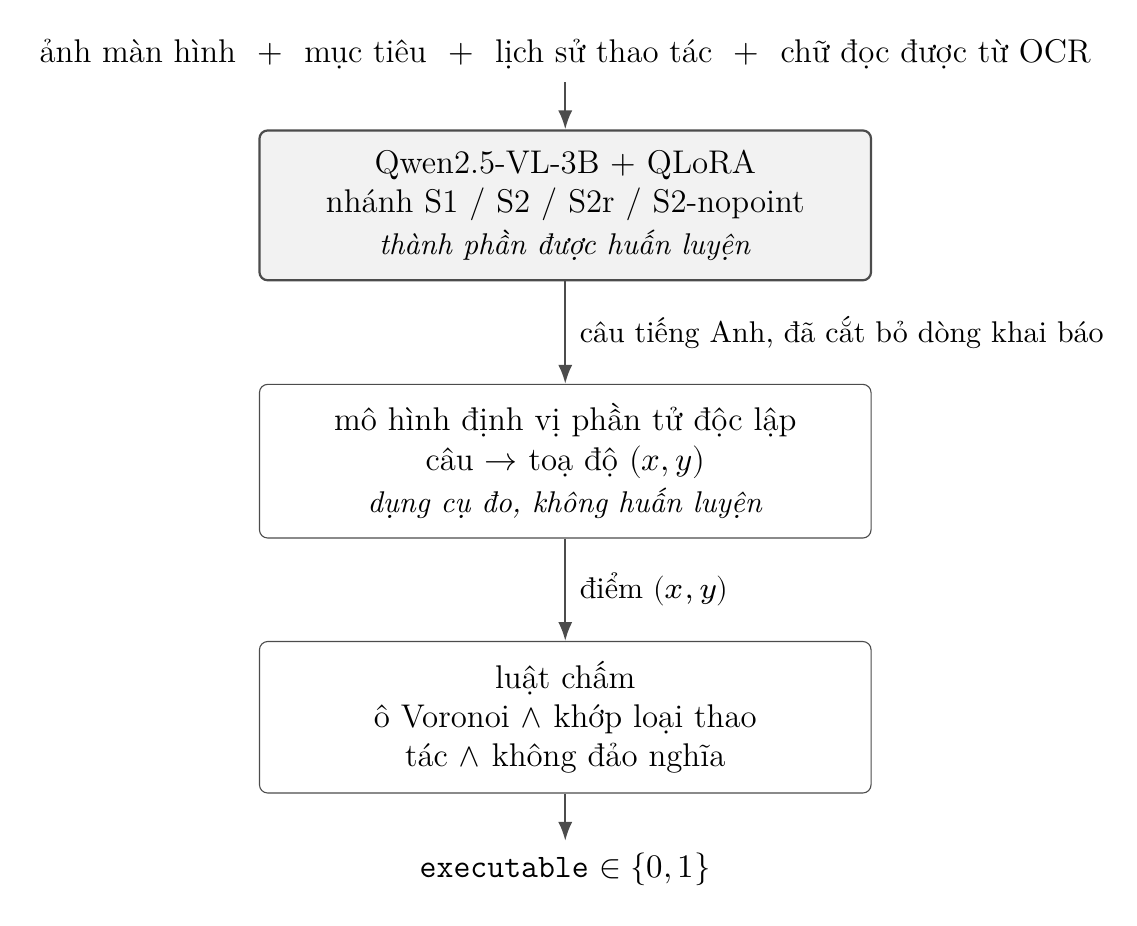
\begin{tikzpicture}[
  font=\small,
  blk/.style={draw=black!70, rounded corners=3pt, align=center,
              text width=0.60\textwidth, inner sep=7pt, fill=white},
  huanluyen/.style={blk, fill=black!5, thick},
  dongoc/.style={align=center, font=\small},
  mui/.style={-{Latex[length=2.4mm]}, draw=black!70, thick},
  nhan/.style={font=\footnotesize, inner sep=2pt, midway, right=1mm},
  vai/.style={font=\footnotesize\itshape}
]
\node (vao) [dongoc] {ảnh màn hình\ \ $+$\ \ mục tiêu\ \ $+$\ \ lịch sử thao tác\ \ $+$\ \ chữ đọc được từ OCR};
\node (sinh) [huanluyen, below=6mm of vao]
  {Qwen2.5-VL-3B $+$ QLoRA\\ nhánh S1 / S2 / S2r / S2-nopoint\\[1pt]
   \textit{\footnotesize thành phần được huấn luyện}};
\node (dinhvi) [blk, below=13mm of sinh]
  {mô hình định vị phần tử độc lập\\ câu $\rightarrow$ toạ độ $(x, y)$\\[1pt]
   \textit{\footnotesize dụng cụ đo, không huấn luyện}};
\node (cham) [blk, below=13mm of dinhvi]
  {luật chấm\\ ô Voronoi $\wedge$ khớp loại thao tác $\wedge$ không đảo nghĩa};
\node (ra) [dongoc, below=6mm of cham] {\code{executable} $\in \{0, 1\}$};

\draw [mui] (vao) -- (sinh);
\draw [mui] (sinh) -- node[nhan] {câu tiếng Anh, đã cắt bỏ dòng khai báo} (dinhvi);
\draw [mui] (dinhvi) -- node[nhan] {điểm $(x, y)$} (cham);
\draw [mui] (cham) -- (ra);

\end{tikzpicture}
\caption{Bốn mắt xích của hệ thống. Khối tô xám là phần duy nhất được huấn luyện; hai khối
dưới thuộc phần đo lường và không bao giờ thấy toạ độ đáp án.}
\label{fig:pipeline}
\end{figure}

Hình~\ref{fig:pipeline} còn cho thấy một điểm về triển khai. Lúc chạy thật, hệ
thống chỉ cần bộ đọc chữ và mô hình đã tinh chỉnh. Cây trợ năng và mô hình định vị chỉ tồn tại ở khâu
dựng dữ liệu và khâu chấm điểm, không có mặt trong đường chạy tới người dùng.

\section{Đầu vào và câu nhắc}

Câu nhắc được ghép từ bốn mảnh và \textbf{giống hệt nhau từng byte ở mọi nhánh cũng như
lúc suy luận}. Đây là điều kiện để chênh lệch điểm quy được về can thiệp. Khối dưới đây
là một câu nhắc thật.

\begin{quote}\ttfamily\footnotesize
<image>\\
Mục tiêu: Open Google maps app, Search for the nearest\\
\hspace*{1em}park to 98103 \ldots\\
Đã làm: Click on the title of this note Grocery to edit\\
\hspace*{1em}the title\\
Chữ đọc được trên màn: Search here $\cdot$ Coffee $\cdot$\\
\hspace*{1em}Restaurants $\cdot$ Groceries $\cdot$ \ldots\\
Viết câu hướng dẫn cho bước tiếp theo.
\end{quote}

Nhãn trường được viết bằng tiếng Việt kèm chỉ thị trả lời bằng tiếng Anh, là ngôn ngữ của
bộ ngữ liệu nguồn và của mọi câu được chấm.

Việc đưa danh sách chữ OCR vào đầu vào nhắm vào dạng lỗi đã đo được là gọi sai
hoặc gọi mơ hồ tên nút. \textbf{Tầng này không được kể là đóng góp.} Chính
nhóm tác giả AndroidControl đã tinh chỉnh với danh sách phần tử làm đầu
vào~\cite{androidcontrol}, và Widget Captioning~\cite{widgetcap},
Screen2Words~\cite{screen2words}, Mind2Web~\cite{mind2web} cũng vậy. Nó là một lựa chọn
thiết kế, và có nhánh đối chứng đi kèm.

Trường ``Đã làm'' chứa \emph{câu do người viết} ở các bước trước, không phải nhật ký thao
tác của chính mô hình. Ở mỗi bước, mô hình được cho sẵn một ngữ cảnh đúng thay vì phải tự dựng lấy ngữ cảnh từ
những gì nó đã sinh ra, đúng theo lối đánh giá quen gọi là \emph{teacher forcing}. Trường này là hằng số của thí nghiệm nên không giải
thích được chênh lệch giữa các nhánh, nhưng nó đặt văn phong của người chú thích vào đầu
vào, và mọi điểm số tuyệt đối đều có điều kiện trên đó.

\section{Mô tả phân biệt trước, phát ngôn sau}

Thay vì dạy mô hình nhảy thẳng từ ảnh sang câu, luận văn dạy nó mô tả phần tử cần chạm trước
rồi mới viết câu. Chuỗi mà mô hình phải sinh ra vì vậy có hai tầng, trình bày ở khối dưới
đây.

\begin{center}\small
\renewcommand{\arraystretch}{1.4}
\begin{tabular}{@{}r@{\ \ }l@{}}
\textit{tầng khai báo} &
\code{<desc>} vai trò \code{|} tên \code{|} \code{<point>}$x,y$\code{</point>}\\
& \code{|} dấu hiệu phân biệt \code{</desc>} \\
\textit{tầng phát ngôn} & câu hướng dẫn \\
\end{tabular}
\end{center}

Lúc chấm, tầng khai báo bị \textbf{cắt bỏ}; chỉ câu hướng dẫn được đưa cho mô hình định
vị. Điều này quan trọng về mặt phân loại đóng góp. Nếu điểm số tăng thì không phải vì mô hình
được cho thêm thông tin lúc chấm, mà vì \emph{hành vi nội tại lúc suy luận đã đổi}.
Đó là điều kiện để gọi đây là đóng góp về mô hình chứ không phải đóng góp về dữ liệu.

Thiết kế này dựa trên ba căn cứ, xếp theo mức độ vững chắc giảm dần.

\begin{enumerate}[leftmargin=1.6em]
\item \textbf{Dạng lỗi đã đo được là câu mơ hồ}, không phải bịa đặt
(Mục 1.1). Một dòng khai báo bắt buộc có ô ``dấu hiệu phân biệt'' nhắm vào đó.

\item \textbf{Bước trung gian phải có cấu trúc và có toạ độ.} Cặp Shikra trong
Bảng~\ref{tab:tienle} là bằng chứng sạch nhất, vì cặp này dùng cùng mô hình và cùng bài
kiểm, chỉ đổi dạng bước trung gian. Viết bằng văn xuôi cho $-7{,}4$, còn viết có toạ độ
cho $+5{,}9$. Vì vậy dòng khai báo
được ràng buộc thành bốn ô cố định và bắt buộc có ô toạ độ.

\item \textbf{Nhãn toạ độ sạch $100\%$ và chi phí dựng bằng không.} Toạ độ chạm của người
thật có sẵn trong dữ liệu; đây là nguồn giám sát mà tinh chỉnh thông thường không dùng tới.
\end{enumerate}

\paragraph{Không dùng chữ ``đầu tiên''.} Như đã nêu ở Mục 1.4.2, ý ``câu phải đủ để bên
kia trỏ đúng'' đã thuộc về dòng sinh biểu thức quy chiếu từ $2016$~\cite{mao2016,luo2017,yu2017}.
Phần được nhận ở đây hẹp hơn nhiều. Luận văn chỉ đưa tính phân biệt vào đích huấn luyện
\emph{trong miền giao diện}, nơi công trình có giám sát gần nhất vẫn dùng entropy chéo
thuần~\cite{widgetcap}.

\section{Cấu hình huấn luyện}
\label{sec:cauhinh}

Mọi nhánh tinh chỉnh Qwen2.5-VL-3B-Instruct~\cite{qwen25vl} bằng QLoRA~\cite{lora,qlora}
dưới LLaMA-Factory~\cite{llamafactory}. Bảng~\ref{tab:cauhinh} liệt kê cấu hình đầy đủ.

\begin{table}[t]
\caption{Cấu hình huấn luyện. Một tệp cấu hình duy nhất phục vụ mọi nhánh và chỉ ba dòng
thay đổi giữa các nhánh, gồm tập dữ liệu, hạt giống và thư mục đầu ra.}
\label{tab:cauhinh}
\centering\small
\renewcommand{\arraystretch}{1.15}
\begin{tabular}{@{}p{5.6cm}p{7.2cm}@{}}
\toprule
Tham số & Giá trị \\
\midrule
Mô hình gốc & Qwen2.5-VL-3B-Instruct \\
Lượng tử hoá & NF4, $4$ bit \\
Hạng LoRA $r$ / $\alpha$ / dropout & $8$ / $16$ / $0{,}05$ \\
Mô-đun gắn bộ chuyển đổi & \code{q,k,v,o,gate,up,down} \\
Tháp thị giác, tầng chiếu đa phương thức & đóng băng \\
Độ dài ngữ cảnh & $2560$ \\
Cỡ lô mỗi thiết bị / tích luỹ gradient & $4$ / $4$ (hiệu dụng $16$) \\
Tốc độ học / lịch / tỉ lệ khởi động & $1\times10^{-4}$ / cosine / $0{,}05$ \\
Số lượt duyệt & $2$ ($=8.072$ bước) \\
Độ chính xác & bf16, có gradient checkpointing \\
Nhân hợp nhất & có bật \\
Tiến trình tiền xử lý & $8$ \\
Hạt giống & $101$ và $202$ \\
Phần cứng & một card A100 \\
\midrule
\textbf{Tham số huấn luyện được} & \textbf{$14.966.784$} ($0{,}48\%$ phần ngôn ngữ) \\
\bottomrule
\end{tabular}
\end{table}

\paragraph{Độ dài ngữ cảnh được nâng trước lượt chạy đầu.} Mẫu S2 dài nhất đạt $2.017$
token, chỉ còn dư $31$ token so với giới hạn $2048$ ban đầu. Việc cắt bớt sẽ diễn ra
\emph{im lặng} và lệch đúng theo hướng bất lợi nhất, vì khung huấn luyện cắt từ đuôi, mà
đuôi chính là chuỗi mô hình phải sinh ra, mà chuỗi của S2 thì dài hơn. Giới hạn được nâng lên
$2560$; vì đệm tính theo từng lô, không theo trần, nên việc nâng này không tốn thêm gì.

\paragraph{Hai phép kiểm cơ học chạy trước mỗi lượt.} Số tham số huấn luyện được phải
đúng $14.966.784$; và tệp cấu hình của lượt hiện tại được đối chiếu từng khoá với lượt
tham chiếu, chỉ bốn khoá được phép khác (hạt giống, thư mục đầu ra, tập dữ liệu, số tiến
trình tiền xử lý), khoá thứ năm khác nhau là dừng hẳn. Ba khoá đầu là ba dòng nói ở
caption Bảng~\ref{tab:cauhinh}; khoá thứ tư chỉ đổi tốc độ tiền xử lý, không đổi dữ liệu ra.

\paragraph{Hai phép kiểm cho những phần mà người đọc không tự kiểm được.} Thứ nhất, cùng hạt
giống $101$, hàm mất mát $20$ bước đầu trên card L4 và trên card A100 khớp tới ba chữ số
($2{,}036$ / $0{,}9686$ / $0{,}8635$ / $0{,}9553$ so với $2{,}040$ / $0{,}9679$ /
$0{,}8635$ / $0{,}9547$) và tổng khối lượng tính toán giống hệt, nghĩa là đổi phần cứng không
đổi kết quả. Thứ hai, sinh câu ở cỡ lô $1$ và cỡ lô $8$ cho đầu ra trùng nhau từng byte,
xác nhận việc đệm bên trái được cài đúng.

\section{Các nhánh đăng ký và thiết kế so sánh}
\label{sec:nhanh}

Bảy nhánh được đăng ký, tất cả dùng chung dữ liệu, mô hình gốc, siêu tham số và tập
kiểm. Bảng~\ref{tab:nhanh} liệt kê từng nhánh cùng câu hỏi mà nó trả lời.

\begin{table}[t]
\caption{Các nhánh đã đăng ký và vai trò của từng nhánh. Ba nhánh cuối không cần huấn
luyện.}
\label{tab:nhanh}
\centering\small
\renewcommand{\arraystretch}{1.2}
\begin{tabular}{@{}p{2.7cm}p{4.4cm}p{5.9cm}@{}}
\toprule
Nhánh & Chuỗi phải sinh ra hoặc cách chạy & Trả lời câu hỏi \\
\midrule
\textbf{S1} & câu trơn ($2$ hạt giống) & nền so sánh nội bộ \\
\textbf{S2} & khai báo thật $+$ câu ($2$ hạt giống) & \textbf{câu hỏi chính} của thiết kế,
là thành phần đề xuất có tác dụng hay không \\
\textbf{S2r} & khai báo giả khớp độ dài $+$ câu & điểm tăng có phải chỉ vì chuỗi phải sinh
ra dài thêm \\
\textbf{S2-nopoint} & khai báo bỏ ô toạ độ $+$ câu & phần công thuộc về ô toạ độ là bao
nhiêu \\
\midrule
\textbf{B-infer} & trọng số S1, danh sách phần tử nhét vào đầu vào lúc chạy & huấn luyện
có hơn việc đưa thông tin lúc chạy không \\
\textbf{Base} & mô hình gốc, không tinh chỉnh & bản thân tinh chỉnh mua được bao nhiêu \\
\textbf{Trần} & câu do người viết đưa thẳng đi chấm & trần của thước đo \\
\bottomrule
\end{tabular}
\end{table}

Đại lượng quan tâm là $\Delta = \text{S2} - \text{S1}$. Cặp hạt giống của S1 cung cấp
\textbf{null thực nghiệm}. Chênh lệch giữa hai lượt chạy của cùng một thiết kế chính là
sàn nhiễu mà $\Delta$ phải vượt qua. Không có con số đó thì không phân biệt được ``S2 hơn
S1'' với ``hai lượt huấn luyện vốn đã khác nhau chừng đó''.

Trình tự thực hiện được khoá cứng và không được đảo, theo đúng sơ đồ dưới đây.
\begin{center}
S1 $\times 2$ hạt giống $\rightarrow$ chấm đủ $\rightarrow$ đo MDE thật $\rightarrow$
khoá ngưỡng $\rightarrow$ \emph{mới} huấn luyện S2.
\end{center}

Bản đăng ký cam kết trước rằng một mức tăng của riêng S2 \textbf{không} được quy cho tính
phân biệt nếu chưa đi qua S2r và S2-nopoint.

\paragraph{Bảng này mô tả thiết kế, không mô tả các lượt đã chạy.} Trong bảy nhánh trên, hạt
giống thứ hai của S2 cùng ba nhánh S2r, S2-nopoint và B-infer không được chạy. Lý do của
từng nhánh, gồm ngân sách máy với nhánh thứ nhất và lý do đo được với ba nhánh còn lại, ghi
ở Bảng~\ref{tab:trangthai}. Hệ quả trực tiếp là đại lượng $\Delta$ định nghĩa ở đây không
hoàn tất; luận văn giữ nguyên định nghĩa thay vì sửa nó cho vừa với dữ liệu có được.

\paragraph{B-infer là mốc so yếu hơn tên gọi của nó.} Phần này nêu trước để không đọc quá lời một kết quả cao hơn của nhánh huấn luyện. Câu nhắc của B-infer dài trung vị $1.149$
token so với $486$ của vùng đã huấn luyện, danh sách phần tử bị cắt còn $40$ trong khi màn
hình có trung vị $72$ phần tử, và chỉ $14{,}1\%$ phần tử trong danh sách có tên. Nếu nhánh này thấp hơn thì không kết luận được gì.

\section{Chặng huấn luyện thứ hai với mục tiêu ưu tiên ở tầng khai báo}
\label{sec:mindescthietke}

Mục này mô tả một chặng huấn luyện \emph{ra đời sau} bản đăng ký gốc. Chặng này được ghi thành mục sửa đổi có ngày $23$ tháng $8$, trước khi tồn tại bất kỳ
điểm số nào, và được trình bày ở đây vì nó nối thẳng vào chẩn đoán mà nhánh S2 để lại.

\paragraph{Căn cứ của chặng huấn luyện này.} Nhánh S2 cho thấy một cơ chế tác động theo hai chiều
ngược nhau. Khi ô khai báo do mô hình tự sinh trỏ đúng phần tử, câu viết ra tốt hơn nhánh
chỉ sinh câu $5{,}7$ điểm; còn khi ô đó trỏ sai cả tên lẫn toạ độ, nó thấp hơn tới $25{,}2$ điểm (Mục~\ref{sec:o2x2s2}). Điểm nghẽn vì vậy không nằm ở việc \emph{có} tầng khai
báo hay không, mà ở \emph{độ chính xác} của tầng ấy. Học có giám sát thuần không tác động
thẳng vào việc chọn phần tử, vì nó chỉ nâng xác suất của chuỗi đúng chứ không hạ xác suất
của chuỗi sai gần kề.

\paragraph{Cặp quy chiếu tối thiểu.} Từ chính điểm lưu của nhánh S2, chặng hai huấn luyện thêm
$800$ bước cập nhật bằng một mục tiêu ưu tiên trên các cặp có dạng như sau.

\begin{center}\small
\begin{tabular}{@{}ll@{}}
vế được chọn & \code{<desc>}khai báo đúng\code{</desc>} $+$ \code{\textbackslash n} $+$ câu \\
vế bị loại & \code{<desc>}khai báo sai\code{</desc>} $+$ \code{\textbackslash n} $+$ \emph{đúng câu đó} \\
\end{tabular}
\end{center}

Hai vế \textbf{chỉ khác nhau ở ô khai báo}; phần câu giống nhau từng chữ. Vì vậy số hạng ưu
tiên chỉ có thể giảm bằng cách chọn đúng phần tử; nó không giảm được bằng cách đổi văn
phong, đổi độ dài hay viết một câu nghe trau chuốt hơn. Khai báo sai lấy từ phần tử cùng vai trò gần
nhất, cách điểm chạm thật từ $80$ đến $350$ điểm ảnh, tức một phần tử thật trên chính màn
hình đó chứ không phải một chuỗi bịa ra. Tập cặp gồm $22.854$ cặp và phải đi qua bảy bất
biến cấu trúc kiểm tự động; chương trình dựng dữ liệu dừng hẳn nếu có bất biến nào trượt.

Hàm mục tiêu ở đây thuộc họ tối ưu theo ưu tiên dạng tỉ số odds (ORPO). Trong họ này, số
hạng phạt vế bị loại được cộng thẳng vào hàm mất mát có giám sát của vế được chọn, thay vì đo độ lệch so với
một mô hình tham chiếu đóng băng như cách làm thông dụng của các phương pháp tối ưu theo ưu
tiên. Nhờ vậy chỉ cần giữ \emph{một} bản trọng số trong bộ nhớ thay vì hai, và đây là điều
kiện bắt buộc để chặng này chạy vừa trên một card đồ hoạ đơn với cùng cấu hình lượng tử hoá
bốn bit của các nhánh trước.

\paragraph{Đối chứng quy công.} Một chặng huấn luyện thêm $800$ bước tự nó đã làm mô hình
đổi, bất kể mục tiêu là gì. Để tách phần thuộc về mục tiêu ưu tiên, nhánh đối chứng
\textbf{CE2-S2} chạy học có giám sát thuần trên \emph{riêng vế được chọn} của đúng những
cặp ấy. Nhánh này giữ nguyên điểm lưu xuất phát, số bước cập nhật và lịch tốc độ học của
chặng hai, chỉ bỏ đi số hạng ưu tiên. Đại lượng đăng ký cho chặng này là hiệu ghép cặp
$\Delta_{\text{thành phần}} = \text{MIN-DESC} - \text{CE2-S2}$, và luật đọc là luật ở
Bảng~\ref{tab:luatdoc} không sửa một chữ.

\paragraph{Hai điểm chệch khỏi thiết kế gốc.} Thứ nhất, tập cặp chỉ
chứa \emph{bước chạm}, vì chỉ bước chạm mới có nhãn khai báo; mức thiệt hại của việc đó đo
được ở Mục~\ref{sec:khongcham}. Thứ hai, chặng này chỉ chạy được một hạt giống, nên theo đúng luật
đã khoá, kết quả của nó là thăm dò bất kể con số ra sao.

\section{Bản đăng ký trước và luật đọc kết quả}
\label{sec:dangky}

Toàn bộ thiết kế được đưa vào kho phiên bản \emph{trước} lượt huấn luyện đầu tiên, và
quy định cách đọc cả bốn kết cục có thể xảy ra (Bảng~\ref{tab:luatdoc}). Mọi thay đổi về
sau được ghi thành mục sửa đổi có ngày ở cuối văn bản, không sửa đè lên bản gốc; phần lớn
các mục này ra đời trước khi tồn tại bất kỳ điểm số nào.

\begin{table}[t]
\caption{Luật đọc kết quả, viết trước khi thấy số.}
\label{tab:luatdoc}
\centering\small
\renewcommand{\arraystretch}{1.25}
\begin{tabular}{@{}p{5.4cm}p{7.4cm}@{}}
\toprule
Kết cục & Kết luận được phép viết \\
\midrule
$\Delta$ vượt MDE và cận dưới KTC $> 0$ & thành phần có tác dụng \\
KTC chạm $0$ & xu hướng; \emph{không} được gọi là cải thiện \\
KTC phủ $0$ và $|\Delta|$ dưới MDE & kết quả âm có kiểm soát, báo thẳng \\
Cận trên KTC $< 0$ & thành phần gây hại, báo thẳng \\
\bottomrule
\end{tabular}
\end{table}

Ba lát cắt phân tích, tức ba cách chia quần thể thành các nhóm nhỏ để đọc kết quả riêng
trên từng nhóm, được cho phép báo cáo và đã công bố trước. Ba cách chia đó là theo độ dài
câu, theo độ khó của màn hình và theo nguồn của tên phần tử. Bất cứ lát cắt nào tìm ra sau khi thấy số đều
là thăm dò và phải ghi rõ như vậy.

\paragraph{Một mục sửa đổi về ngưỡng MDE.} Ngưỡng MDE ban đầu được \emph{chiếu} chứ không
được đo, và công thức dùng để chiếu giả định tương quan trong cụm bằng một. Khi đo thật
thì hệ số nở do gom cụm chỉ là $1{,}10$, nên công thức cũ thổi phồng ngưỡng lên khoảng
ba lần và sẽ khiến một hiệu ứng thật $3$ điểm bị tuyên là ``không kết luận được'' trong
khi khoảng tin cậy của nó loại trừ $0$ ở mức $p < 0{,}001$. Ngưỡng được sửa thành sai số
chuẩn ghép cặp đo được, và mục sửa đổi này được ghi \emph{trước} khi chấm bất kỳ nhánh xử
lý nào (Mục~\ref{sec:thongke}).

\section{Mức hai và khoản phạt cho câu vẫn mơ hồ}

Thiết kế còn một tầng nữa đã đăng ký nhưng \textbf{chưa cài đặt}.

Ý tưởng của tầng này như sau. Khi màn hình có hai phần tử giống hệt nhau, chẳng hạn hai
biểu tượng kính lúp, thì câu ``Tap the search icon'' khớp với cả hai và vì vậy là câu mơ hồ. Ô mô tả phần tử hàng xóm gần nhất đã được dựng sẵn trong nhãn; hàm mất mát
mức hai sẽ phạt khi mô hình gán cho khai báo thật một xác suất không cao hơn khai báo
hàng xóm ít nhất một khoảng lề định trước. Đây đúng là chỗ Widget Captioning~\cite{widgetcap} còn để trống, nơi vấn đề được nêu ra
nhưng hàm mất mát vẫn là entropy chéo thuần.

Hiện tại, dữ liệu đã sẵn sàng nhưng \emph{mã hàm mất mát chưa được viết}. Tầng này nằm
sau một điều kiện chặn riêng và chỉ được mở nếu tầng một cho tín hiệu. Nếu không kịp chạy thì trạng
thái đúng của nó là \emph{đã đăng ký nhưng không thực hiện}.

\chapter{Thước đo executability}
\label{ch:thuocdo}

Chương~\ref{ch:tongquan} đã chỉ ra rằng câu hỏi ``câu sinh ra có giống câu chuẩn không''
không trả lời được một cách đáng tin. Chương này thay nó bằng câu hỏi ``câu sinh ra có
dẫn được tới đúng phần tử không'', định nghĩa thước đo tương ứng, rồi dành phần lớn dung
lượng để \emph{kiểm chứng chính thước đó} trước khi dùng nó kết luận bất cứ điều gì.

\section{Định nghĩa}
\label{sec:dinhnghia}

Gọi $s$ là câu sinh ra sau khi đã cắt bỏ dòng khai báo, $I$ là ảnh màn hình, $g$ là toạ
độ chạm của người dùng, và $E$ là tập phần tử trên màn lấy từ cây trợ năng sau khi gộp
các phần tử có tâm cách nhau dưới $24$\,dp. Gọi $G$ là một mô hình định vị phần tử, độc
lập với mô hình đang bị chấm và không hề thấy $g$, trả về một điểm $p = G(I, s)$.

Bước được tính \textbf{đúng} khi cả ba điều kiện đồng thời thoả:

\begin{description}[leftmargin=2.2em,style=nextline]
\item[(i) Khớp loại thao tác.] Loại thao tác chuẩn hoá của $s$ và của câu chuẩn phải
trùng nhau. Phép chuẩn hoá gộp mười hai động từ bề mặt (\emph{tap, click, press, select,
choose, touch, open, launch, go, navigate, visit, view}) về một lớp duy nhất, vì trên màn
hình tất cả đều chỉ một cú chạm. Năm lớp còn phân biệt là chạm, gõ, cuộn, nhấn giữ và
quay lại.

\emph{Một lỗi đã biết của cài đặt này phải nêu ngay tại đây.} Vòng quét chạy từ trái sang
phải, mà \emph{go} và \emph{navigate} (đều thuộc lớp chạm) đứng trước \emph{back} trong
câu, nên \emph{go back}, \emph{navigate back} và \emph{press the back button} đều được quy
về chạm; lớp ``quay lại'' vì thế gần như không đạt tới được bằng ba cách nói tự nhiên nhất
của nó. Ảnh hưởng đã đo trên quần thể chấm: $81$ bước đổi phán quyết ở S1, $47$ ở Base và
$0$ ở nhánh câu người viết, kéo điểm từ $59{,}12$ xuống $58{,}81$ và từ $47{,}60$ xuống
$47{,}40$, còn chênh lệch giữa hai nhánh gần như không đổi ($11{,}52$ xuống $11{,}41$
điểm). Ba nhánh đã chấm \textbf{không được chấm lại}: sửa thước sau khi đã thấy điểm đúng
là thứ mà bản đăng ký trước sinh ra để chặn, kể cả khi việc sửa làm số xấu đi. Bản vá đã
viết và bật bằng tham số \code{strict\_back}; nó \textbf{bắt buộc} cho phép kiểm
không-gây-hại, vì phép kiểm đó chạy trên nhóm bước không chạm, nơi thao tác quay lại là
thật, và phép kiểm đó chưa chạy lần nào.

\item[(ii) Không đảo nghĩa.] $s$ và câu chuẩn không được gọi tên hai trạng thái ngược
nhau của cùng một điều khiển. Đây là chỗ duy nhất mà kênh toạ độ mù hoàn toàn: nút ``bật
thông báo'' và ``tắt thông báo'' nằm ở cùng một vị trí chạm. Phép kiểm dùng bảng viết tay
gồm chín cặp (\emph{on/off, enable/disable, show/hide, mute/unmute, expand/collapse,
check/uncheck, select/deselect, start/stop, enabled/disabled}) sau khi đã loại các từ chỉ
vị trí.

\item[(iii) Định vị đúng.] $p$ nằm trong vùng dung sai quy ước quanh $g$,
$|p_x - g_x| \le \tau W$ và $|p_y - g_y| \le \tau H$ với $\tau = 0{,}14$
theo~\cite{aitw}, \emph{và} không phần tử nào khác có tâm gần $p$ hơn chính $g$:
\begin{equation}
\lVert p - g \rVert < \lVert p - c(e) \rVert \quad \forall e \in E,
\label{eq:voronoi}
\end{equation}
với $c(e)$ là tâm của phần tử $e$.
\end{description}

Điểm executability là tỉ lệ bước chạm thoả cả ba điều kiện.

Điều kiện (iii) có hai chi tiết rất dễ phát biểu sai. Thứ nhất, vùng dung sai là một \emph{hình chữ nhật} tính theo từng trục như
trong~\cite{aitw}, không phải một đĩa tròn: trên màn $1080 \times 2400$ nó là $\pm151$
điểm ảnh theo chiều ngang nhưng $\pm336$ điểm ảnh theo chiều dọc, tức là rộng theo chiều
dọc gấp hơn hai lần.

Thứ hai, hạt sinh ra ô Voronoi của phần tử đích là \emph{chính điểm chạm} $g$, không phải
tâm của phần tử chứa $g$. Lý do rất cụ thể: nếu lấy tâm hộp làm hạt thì hộp của chính
phần tử đích sẽ ``gần $g$ hơn $g$'' và bác nhầm những câu đúng: đo được là bác nhầm
$59\%$ số câu cùng nghĩa. Cách xử đúng bản chất là coi \emph{mọi hộp chứa điểm} $g$ đều
thuộc về phần tử đích và loại chúng khỏi danh sách đối thủ.

\paragraph{Đây không phải thiết kế ``mô hình tự chấm''.} Barem là một toạ độ mà người
thật đã chạm, có sẵn trong dữ liệu, không phải ý kiến của một mô hình. $G$ chỉ đóng góp
một phép định vị; việc phán quyết đúng sai do hình học so với $g$ quyết định. $G$ không
bao giờ được luận văn tinh chỉnh và không bao giờ thấy $g$.

\paragraph{Thước này đo gì và không đo gì.} Nó đo \emph{câu có xác định đúng phần tử hay
không}. Độ trôi chảy, độ dài, mức hữu ích với người đọc nằm ngoài phạm vi. Đây là một
phạm vi hẹp, và nó được gọi tên rõ ràng ở đây để người đọc khỏi phải tự suy.

\section{Chọn luật trúng: vì sao ngưỡng dung sai quy ước không đủ}
\label{sec:luattrung}

Điều kiện Voronoi có thực sự cần thiết bên cạnh ngưỡng dung sai quy ước hay không? Câu
hỏi này được trả lời bằng đo đạc. Ba luật được so trên $250$ bước
chạm, mỗi luật đo hai lần: một lần đo \emph{trần} bằng cách bơm một độ lệch có kiểm soát
vào một điểm hoàn hảo, và một lần đo \emph{sàn} bằng cách đặt điểm lên phần tử \emph{khác}
gần nhất, tình huống đại diện cho một câu gọi tên sai nút.

\begin{table}[t]
\caption{So sánh luật trúng. Sàn là tỉ lệ cho điểm khi câu chỉ sang một phần tử khác;
luật càng tốt thì sàn càng thấp.}
\label{tab:luattrung}
\centering\small
\renewcommand{\arraystretch}{1.2}
\begin{tabular}{@{}lrrr@{}}
\toprule
Luật & Trần (lệch $3\%$) & Sàn (chỉ sai nút) & Biên độ \\
\midrule
Ngưỡng dung sai quy ước~\cite{aitw} & --- & $84{,}3\%$ & $\approx 16$ điểm \\
\textbf{Ô Voronoi} & $99{,}7\%$ & $\mathbf{2{,}8\%}$ & $\approx 97$ điểm \\
\bottomrule
\end{tabular}
\end{table}

Kết quả ở Bảng~\ref{tab:luattrung} là căn cứ quyết định. Trước một câu gọi tên sai nút,
luật dung sai quy ước \emph{vẫn cho điểm trong $84{,}3\%$ số ca}, để lại biên độ động
khoảng $16$ điểm, quá hẹp để tách một hướng dẫn tốt khỏi một hướng dẫn dở. Luật ô
Voronoi cho $2{,}8\%$, biên độ khoảng $97$ điểm, trong khi vẫn giữ trần $99{,}7\%$ khi
điểm chỉ lệch $3\%$.

Nguyên nhân gốc nằm ở mật độ nút: $63{,}2\%$ số bước có ít nhất một phần tử \emph{khác} nằm
lọt trong vùng dung sai của phần tử đích. Với mật độ nút như vậy, ngưỡng dung sai không
còn phân biệt được gì.

Hai điều kiện đi kèm phải nêu cùng kết quả này. Thứ nhất, sàn $2{,}8\%$ chỉ áp cho câu
chỉ sang một phần tử \emph{riêng biệt}, không áp cho một điểm bị dịch nhẹ ngay bên trong
ô của chính phần tử đích; giới hạn này được đo và báo ở Mục~\ref{sec:bomloi}. Thứ hai,
phép gộp phần tử định nghĩa thế nào là ``riêng biệt'' không miễn phí: nó xoá một tâm đối
thủ ở $96{,}3\%$ số bước, và ở $8{,}2\%$ số bước có ít nhất một tâm bị xoá thuộc về một
phần tử thật sự riêng biệt. Vì vậy điểm theo ngưỡng dung sai \textbf{luôn được báo bên cạnh điểm chính}, nhưng không bao giờ lấy nó làm điểm chính.

\begin{figure}[t]
\centering
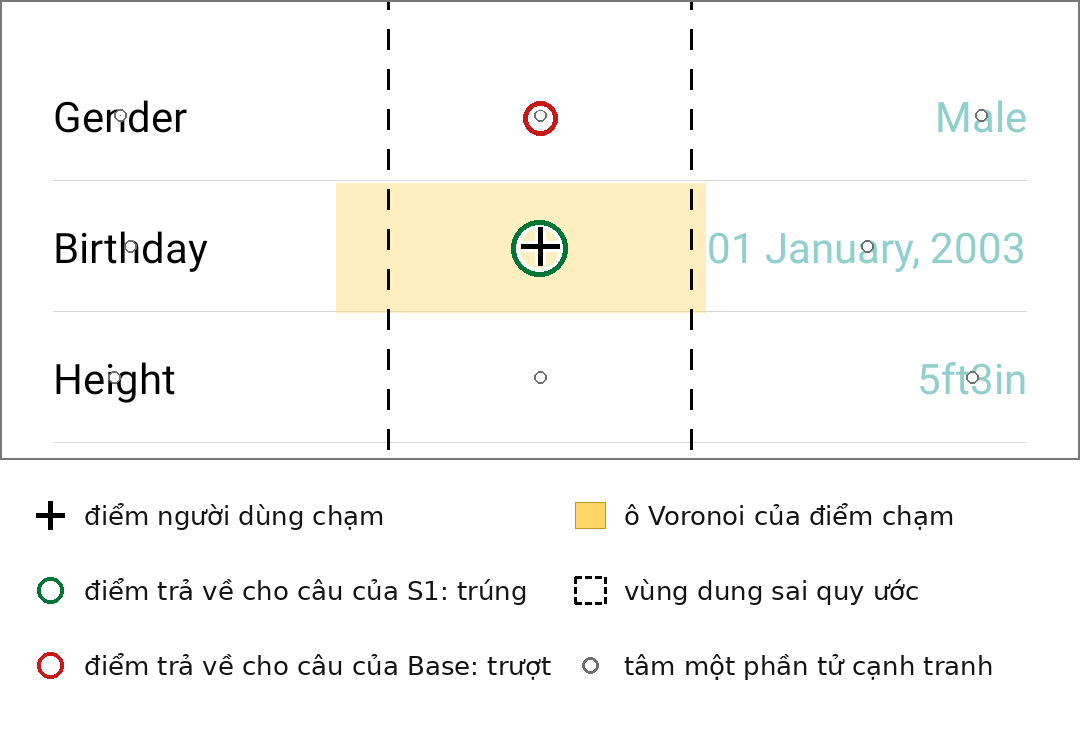
\includegraphics[width=0.72\textwidth]{figures/fig_voronoi.png}
\caption[Một bước mà hai luật chấm bất đồng]{Một bước mà hai luật chấm bất đồng.
Người dùng chạm dòng \emph{Birthday}: vùng tô vàng là \emph{ô Voronoi} của điểm chạm,
khung nét đứt là vùng dung sai quy ước $\pm151 \times \pm336$ điểm ảnh. Dấu chữ thập là
điểm mô hình định vị trả về cho câu của S1, vòng tròn lớn cho câu của Base, các vòng tròn
nhỏ là tâm những phần tử cạnh tranh.}
\label{fig:voronoi}
\end{figure}

Cùng một phán quyết cũng đúng trên dụng cụ thật: chia $300$ bước của phép đo cổng chặn
theo sai số mà mô hình định vị thực sự mắc phải, luật ô Voronoi cho điểm \emph{mọi} bước
có sai số dưới ngưỡng $3\%$ ($n = 188$) và \emph{không} bước nào có sai số trên $14\%$
($n = 63$), trong khi luật dung sai cho điểm tất cả cho tới $14\%$.
Hình~\ref{fig:voronoi} minh hoạ một bước mà hai luật bất đồng. Ở bước đó, mô hình chưa
tinh chỉnh viết ``Click on the `Gender' section\ldots'' và mô hình định vị đi đúng chỗ
được bảo, cách điểm chạm $128$ điểm ảnh về phía dòng trên. Khoảng cách ấy vẫn nằm trong
dung sai $\pm336$ điểm ảnh theo chiều dọc, nên luật quy ước chấm bước này là đúng, còn
luật ô Voronoi thì không.

\section{Mô hình định vị dùng làm dụng cụ đo}
\label{sec:botro}

Dụng cụ đo được chọn là \textbf{UGround-V1-2B}~\cite{uground}, theo ba điều kiện:

\begin{enumerate}[leftmargin=1.6em]
\item khác họ với mô hình bị chấm, để thước không thiên vị;
\item công thức huấn luyện không chứa AndroidControl, để giám khảo không phải là người
đã học chính đề thi;
\item sai số định vị đủ nhỏ, tức cổng chặn ở Mục~\ref{sec:congA}.
\end{enumerate}

Điều kiện thứ ba đạt. \textbf{Hai điều kiện đầu thì không}, và cần nói rõ: UGround-V1-2B được dựng trên Qwen2-VL, cùng dòng với Qwen2.5-VL-3B
đang bị chấm; và bảng thành phần dữ liệu của nó liệt kê $47$ nghìn phần tử có nhãn người
lấy từ \emph{split train} của AndroidControl. Tập kiểm của luận văn tách rời ở mức màn
hình nên đây không phải rò rỉ nhãn, nhưng dụng cụ đo đã thấy \emph{văn phong chú thích}
của bộ ngữ liệu này. Mục~\ref{sec:hanche} xử lý điều đó như một cách giải thích thay thế
còn sống.

Hai chi tiết vận hành đáng ghi lại vì chúng quyết định tính khả thi về chi phí. Câu nhắc
đưa cho $G$ được bê nguyên văn từ thẻ mô hình chính chủ; tự viết lại câu nhắc, nhất là
bằng tiếng Việt, làm nó định vị tệ đi, và khi đó cổng chặn sẽ rớt vì một lý do sai. Và
tham số \code{use\_cache} được khai báo tường minh là bật, không để mặc định quyết: cấu hình
sinh của mô hình đặt nó là tắt, khiến việc sinh $32$ token mất $38{,}7$ giây thay vì
$4{,}2$ giây, chậm $9{,}3$ lần cho một phép biến đổi bảo toàn kết quả. Việc bảo toàn
kết quả ở đây được kiểm bằng thực nghiệm: chạy lại $50$ bước với bộ nhớ đệm bật cho toạ độ
trùng tuyệt đối $50/50$. Nhờ đó chi phí chấm một nhánh giảm từ $48$ giờ xuống $5{,}6$
giờ, vừa hạn mức card đồ hoạ miễn phí, và toàn bộ khâu chấm điểm của luận văn tốn không
đồng nào.

\section{Cổng chặn về sai số của dụng cụ đo}
\label{sec:congA}

Thước kế thừa độ tin cậy của $G$. Trước khi cam kết tài nguyên tính toán, một điều kiện
đạt/không đạt được khoá lại: \textbf{sai số định vị trung vị không quá $3\%$ bề ngang
màn}. Ngưỡng này có căn cứ hình học, không phải một lựa chọn tuỳ ý.

Căn cứ hình học: trên $1.496$ bước chạm, biên dung sai (nửa khoảng cách từ phần tử
đích tới phần tử khác gần nhất sau khi gộp) có trung vị $67$ điểm ảnh ($6{,}2\%$ bề
ngang) và phân vị thứ mười là $39$ điểm ảnh ($3{,}6\%$). Ngưỡng $3\%$ tương ứng khoảng
$32$ điểm ảnh, nằm dưới cả phân vị thứ mười. Bài toán cũng khả thi về nguyên tắc: toạ độ
chạm trong AndroidControl là tâm phần tử, $79{,}4\%$ nằm trong phạm vi $1{,}5$ điểm ảnh
quanh một tâm.

Ngưỡng còn được đối chiếu với hệ quả thực tế của nó (Bảng~\ref{tab:duongcong}): sai số
càng lớn thì thước càng bác nhầm câu đúng.

\begin{table}[t]
\caption{Tỉ lệ bác nhầm câu đúng theo sai số của mô hình định vị, đo bằng dụng cụ thật.}
\label{tab:duongcong}
\centering\small
\begin{tabular}{@{}lrrrr@{}}
\toprule
Sai số (\% bề ngang màn) & $3\%$ & $5\%$ & $8\%$ & $13\%$ \\
\midrule
Tỉ lệ bác nhầm & $0\%$ & $7{,}5\%$ & $24{,}1\%$ & $55\%$ \\
\bottomrule
\end{tabular}
\end{table}

\paragraph{Kết quả đo.} UGround-V1-2B trên $300$ bước tập kiểm với hạt giống cố định cho
sai số trung vị \textbf{$0{,}7\%$} bề ngang màn (phân vị $25$: $0{,}2$; phân vị $75$: $8{,}8$; phân vị $90$: $36{,}3$; $62{,}7\%$ số bước ở mức $3\%$ trở xuống).
\textbf{Cổng đạt}, với biên rộng.

Hai điều phải nói thêm để không đọc quá lời con số này. Thứ nhất, trung vị là một phép
kiểm yếu trên một phân phối lưỡng cực như thế này, vì mô hình định vị hoặc rơi rất gần
tâm hoặc rơi hẳn ra chỗ khác; một điều kiện theo phân vị sẽ là lựa chọn tốt hơn.
Thứ hai, bốn dấu hiệu dò lỗi cài đặt được khai báo trước và \emph{một dấu hiệu đã kích
hoạt}: toạ độ ngang rơi đúng giữa màn ở $30{,}7\%$ số bước, vượt ngưỡng cảnh báo $20\%$.
Truy lại thì một phần là do dữ liệu ($18{,}3\%$ toạ độ đáp án vốn nằm giữa màn), phần còn
lại thì không: trong $245$ bước có đáp án lệch khỏi tâm, mô hình định vị vẫn trả về giữa
màn $46$ lần, trong một dải chỉ chiếm khoảng $1\%$ trục ngang. Khi không
nhận ra được phần tử nào, nó \emph{bỏ cuộc theo trục ngang}. Kiểu hỏng này kéo điểm số
xuống chứ không thổi điểm số lên, nên cổng vẫn đạt một cách chính đáng, nhưng nó được
khai báo lại mỗi lần thước được sử dụng.

\section{Trần của thước đo}
\label{sec:tran}

Cổng chặn đo khoảng cách; thước thì chấm theo ô Voronoi. Để biết điểm cao nhất mà thước
có thể cho một bộ sinh câu hoàn hảo, luận văn đưa \emph{chính câu do người viết} của mọi
bước chạm cho mô hình định vị rồi chấm bằng đúng luật đang triển khai.

Cách làm này có chi phí thấp hơn nhiều so với dự kiến: không cần sinh câu nên \emph{không cần card đồ
hoạ để sinh}, chỉ cần dựng tệp dự đoán với trường \code{pred} bằng chính câu chuẩn rồi
chấm như mọi nhánh khác.

\begin{quote}
Trên toàn bộ $4.463$ bước chạm, $1.091$ cụm (hiệu dụng $454{,}3$), trần là
\textbf{$75{,}7\%$}, KTC 95\% $[74{,}1; 77{,}3]$ theo luật ô Voronoi, và $84{,}3\%$
$[82{,}9; 85{,}6]$ theo ngưỡng dung sai báo kèm. Con số $84{,}3\%$ này trùng số học với sàn
của luật dung sai ở Mục~\ref{sec:luattrung}; hai đại lượng đo trên hai quần thể khác nhau
($4.463$ bước so với $250$ bước) và sự trùng nhau là ngẫu nhiên.
\end{quote}

Vì đầu vào chính là câu chuẩn nên hai điều kiện (i) và (ii) thoả trên tất cả trừ ba bước,
nơi luật đảo nghĩa kích hoạt trên một câu chuẩn chứa cả ``on'' lẫn ``off''; do đó trần này
là một điểm số thuần về định vị, sai lệch dưới $0{,}07\%$.

\textbf{Mọi điểm số executability phải đọc trên nền $75{,}7$, không phải trên nền $100$.}
Một nhánh đạt $59{,}1\%$ tức là đạt $78{,}1\%$ của trần.

\paragraph{Vì sao gọi là trần chứ không gọi là chặn trên.} Đây là điểm số của \emph{một
lớp câu cụ thể}: câu do người chú thích viết cho người khác đọc. Một bộ sinh được thưởng
theo thước này về nguyên tắc có thể vượt qua nó bằng cách viết cho mô hình định vị thay
vì viết cho người, với những cách diễn đạt không ai yêu cầu. Không có gì trong thiết kế
ngăn điều đó, nên một nhánh tiến sát $75{,}7$ phải được đọc là lý do để đi soi câu của nó
chứ không phải là một thành công.

\paragraph{Một con số đã bị rút.} Ước lượng trước đó, tính từ $300$ đầu ra của mô hình
định vị còn giữ lại từ phép đo cổng chặn, cho $70{,}0\%$ $[64{,}5; 75{,}3]$, thấp hơn
$5{,}7$ điểm và nằm \emph{ngoài} cận trên khoảng tin cậy của chính nó. Khoảng tin cậy
hẹp lại từ $\pm5{,}4$ xuống $\pm1{,}6$ khi đo trên toàn tập. Ước lượng trần vì vậy được đo lại trên toàn bộ
$4.463$ bước thay vì trên mẫu con $300$ bước; chi phí đo lại là $5{,}6$ giờ máy miễn phí.

\section{Sàn của thước đo}
\label{sec:san}

Trần cho biết điểm cao nhất mà thước có thể cho. Nhưng một thang đo có hai đầu, và đầu
còn lại quan trọng không kém: \emph{nếu câu không mang thông tin gì thì mô hình định vị
vẫn trúng bao nhiêu?} Nếu con số đó cao, phần lớn điểm mà thước phát ra là điểm cho
\emph{bức ảnh} chứ không phải cho \emph{câu} --- và toàn bộ ý nghĩa của thước sụp đổ.

Có một dấu hiệu khiến câu hỏi này trở nên cấp bách. Trên $4.462$ bước, \textbf{$40{,}0\%$}
số bước được cả ba nhánh giải đúng, \emph{kể cả mô hình chưa hề tinh chỉnh}. Cách đọc tự
nhiên là: hai phần năm quần thể dễ tới mức ai cũng qua, nên sàn có lẽ nằm quanh $40\%$.

\subsection{Ba nhánh đối chứng}

Luận văn dựng ba nhánh, và \emph{ghi luật đọc kết quả trước khi chấm} (mã
\code{harness/make\_floor.py}):

\begin{itemize}
\item \textbf{Câu rỗng nghĩa} --- mọi bước dùng chung một câu \emph{``Tap the button.''}
      Đây là sàn theo nghĩa đen: điểm mà mô hình định vị đạt được khi câu không nói gì.
\item \textbf{Câu sai màn} --- lấy nguyên câu chuẩn \emph{của một bước khác}, thuộc tác vụ
      khác. Câu thật, đúng văn phong, độ dài khớp (trung vị $34$ ký tự so với $35$), chỉ
      \emph{sai nội dung}. Nhánh này là đối chứng cho nhánh trên: câu ``Tap the button.''
      lặp lại tám trăm lần là một đầu vào \emph{lạc phân bố}, và mô hình định vị có thể
      hành xử bất thường vì nó \emph{lạ} chứ không vì nó \emph{vô nghĩa}.
\item \textbf{Câu bỏ tên} --- giữ nguyên mệnh đề chỉ vị trí, thay tên phần tử bằng từ chung
      ``the item''. Đây là phép nghịch đảo của nhánh bỏ mệnh đề vị trí ở
      phép kiểm diễn đạt lại, và nó trả lời câu hỏi thước đo \emph{gọi tên} hay đo
      \emph{chỉ chỗ}.
\end{itemize}

\subsection{Kết quả}

Đo trên một lát ngẫu nhiên $800$ bước có trần $74{,}9\%$, tức lệch dưới một điểm so với
toàn tập:

\begin{table}[h]
\centering\small
\renewcommand{\arraystretch}{1.25}
\begin{tabular}{@{}llcc@{}}
\toprule
Nhánh & Câu đưa cho mô hình định vị & Điểm & KTC 95\% \\
\midrule
Trần & câu do người viết & $74{,}9$ & --- \\
S1 & mô hình đã tinh chỉnh & $58{,}8$ & --- \\
Base & mô hình chưa tinh chỉnh & $48{,}6$ & --- \\
\midrule
\textbf{Câu rỗng nghĩa} & \emph{``Tap the button.''} & $\mathbf{12{,}0}$ & $[9{,}7; 14{,}4]$ \\
\textbf{Câu sai màn} & câu chuẩn của bước khác & $\mathbf{6{,}1}$ & $[4{,}5; 7{,}9]$ \\
\bottomrule
\end{tabular}
\end{table}

\paragraph{Sàn là $12{,}0\%$, không phải $40\%$.} Dải mà thước thực sự dùng được là
$74{,}9 - 12{,}0 = \mathbf{62{,}9}$ điểm. Suy luận từ tỉ lệ đồng thuận ở đầu mục
\emph{sai}: $40\%$ số bước ấy dễ \emph{khi có câu thật}, không phải dễ vô điều kiện. Mô
hình định vị không tự đoán ra chúng --- nó cần một câu chỉ đúng phần tử, và cả ba nhánh
đều chỉ đúng ở đó. Đọc theo dải dùng được: Base ở $58{,}3\%$, S1 ở $74{,}4\%$.

\paragraph{Câu sai màn còn thấp hơn câu rỗng nghĩa, và điều đó có ý nghĩa.} $6{,}1\%$ so
với $12{,}0\%$, hai khoảng tin cậy không chồng lấn. Đòn phản biện nặng nhất với thước này
là \emph{nhiễm văn phong}: mô hình định vị đã được huấn luyện trên chú thích của chính kho
dữ liệu này (Mục~\ref{sec:botro}), nên có thể nó thưởng cho câu viết đúng văn phong ấy
\emph{bất kể nội dung}. Nhánh câu-sai-màn là phép thử trực tiếp của giả thuyết đó: văn
phong hoàn hảo, độ dài khớp, nội dung sai. Theo giả thuyết nhiễm, nó phải ăn điểm
\emph{cao}. Nó ăn điểm \emph{thấp nhất trong mọi nhánh đã đo}, thấp hơn cả câu vô nghĩa.

Mô hình định vị vì vậy \emph{thật sự đọc câu}: một câu sai dẫn nó đi lạc, còn một câu rỗng
để nó rơi về tiên nghiệm thị giác yếu ớt. Đây là hành vi của một dụng cụ đang đo
\emph{nội dung}, không phải đang đo \emph{phong cách}.

\subsection{Thước đo gọi tên, không đo chỉ chỗ}
\label{sec:goiten}

Hai phép cắt bổ nhau, chạy trên hai quần thể gần bằng nhau nên so trực tiếp được:

\begin{table}[h]
\centering\small
\renewcommand{\arraystretch}{1.25}
\begin{tabular}{@{}lccc@{}}
\toprule
Phép cắt & $n$ & Trần $\to$ sau khi cắt & Tụt \\
\midrule
\textbf{Bỏ TÊN}, giữ vị trí & $193$ & $89{,}6 \to 61{,}1$ & $\mathbf{-28{,}5}$ pp \\
Bỏ VỊ TRÍ, giữ tên & $198$ & $89{,}4 \to 85{,}9$ & $-3{,}5$ pp \\
\bottomrule
\end{tabular}
\end{table}

McNemar trên phép cắt tên: $b = 58$, $c = 3$, $\chi^2 = 47{,}8$, $p < 0{,}001$.
\textbf{Gọi đúng tên phần tử đáng gấp tám lần nói đúng chỗ.}

Đây là bằng chứng thực nghiệm cho tên gọi của bài toán. Nếu con số ngược lại --- bỏ tên
cũng chỉ mất chừng ba điểm như bỏ vị trí --- thì thước này đo \emph{định vị} chứ không đo
\emph{định danh}, và cả cách đặt vấn đề của luận văn phải viết lại.

\paragraph{Một cái bẫy khi đọc con số này.} Nhánh bỏ tên chỉ viết lại được những câu
\emph{có} mệnh đề vị trí, tức $24{,}1\%$ số bước. Trên toàn lát $800$ bước, điểm của nó là
$68{,}0\%$ --- chỉ tụt $6{,}9$ điểm so với trần, nghe như không đáng kể. Con số ấy bị
\emph{pha loãng $4{,}15$ lần} bởi $607$ bước giữ nguyên câu chuẩn. Số phải đọc là số trên
phần bị đụng, $-28{,}5$ điểm. Mọi phép cắt chỉ chạm một phần quần thể đều phải đọc như vậy.

\section{Kiểm chứng bằng bơm lỗi có kiểm soát}
\label{sec:bomloi}

Theo phương pháp danh sách phép bơm lỗi của Sai và cộng sự~\cite{sai2021}, mười tiêu chí
cùng ngưỡng đạt được cố định \emph{trước} khi chạy, trên $398$ bước chạm của tập kiểm.
Kết quả ở Bảng~\ref{tab:bomloi}.

\begin{table}[t]
\caption{Tự kiểm thước bằng lỗi bơm vào. Ngưỡng cố định trước khi thực thi.}
\label{tab:bomloi}
\centering\small
\renewcommand{\arraystretch}{1.15}
\begin{tabular}{@{}lrrrl@{}}
\toprule
Tiêu chí & Ngưỡng & Đo được & $n$ & \\
\midrule
Kết oan câu diễn đạt khác & $\le 10\%$ & $0{,}0\%$ & $398$ & đạt \\
Kết oan ở cổng thao tác & $\le 15\%$ & $0{,}0\%$ & $398$ & đạt \\
Kết oan ở luật đảo nghĩa & $\le 5\%$ & $0{,}0\%$ & $398$ & đạt \\
Bắt được phần tử kề gần & $\ge 80\%$ & $33{,}1\%$ & $121$ & \textbf{không đạt} \\
Bắt được phần tử kề xa & $\ge 90\%$ & $99{,}6\%$ & $233$ & đạt \\
Bắt được phần tử rất xa & $\ge 95\%$ & $100{,}0\%$ & $397$ & đạt \\
Bắt được phủ định ngoài bảng & $\ge 50\%$ & $20{,}0\%$ & $15$ & \textbf{không đạt} \\
Bắt được sai loại thao tác & $\ge 80\%$ & $100{,}0\%$ & $369$ & đạt \\
Bắt được sai nội dung & $\ge 90\%$ & $91{,}1\%$ & $494$ & đạt \\
Bắt được sai hướng & $\ge 90\%$ & $100{,}0\%$ & $755$ & đạt \\
\bottomrule
\end{tabular}
\end{table}

\paragraph{Con số ``8 trên 10'' không được đọc như một độ chính xác.} Luận văn tự phân
tích và chỉ ra rằng \textbf{năm dòng không thể trượt theo cấu tạo}: cổng thao tác hoán đổi
đúng những động từ mà hàm chuẩn hoá coi là tương đương; luật đảo nghĩa chỉ có thể kích
hoạt trên ba câu chuẩn; hai dòng ``sai loại thao tác'' và ``sai hướng'' kiểm một bảng tra
bằng chính bảng đó; và dòng ``diễn đạt khác'' bơm điểm ``đúng'' của nó chỉ cách đáp án
$23$ điểm ảnh, tức nằm trong bán kính gộp. \textbf{Chỉ bốn dòng mang thông tin}, tức những
dòng đặt điểm lên một phần tử kề hoặc phủ định câu, và \emph{hai trong bốn dòng đó
không đạt}.

Chỗ không đạt thứ nhất là hệ quả trực tiếp của một quyết định thiết kế. Thước
không phân biệt được các điểm dịch chuyển dưới khoảng $63$ điểm ảnh, vì luật gộp các phần
tử có tâm cách nhau dưới $24$\,dp ($63{,}1$ điểm ảnh ở mật độ $2{,}625$ của thiết bị rộng
$1080$). Bán kính đó chỉ nhỏ hơn một chút so với biên dung sai trung vị $67$ điểm ảnh ở
Mục~\ref{sec:congA}, nên một độ dịch dưới ngưỡng này thường vẫn nằm trong ô của chính
phần tử đích. Phát biểu chính xác về năng lực của thước vì vậy là: \emph{nó phát hiện
việc gọi tên sai phần tử, và nó không phát hiện việc chỉ hơi lệch bên trong đúng phần
tử}.

\paragraph{Không đạt thứ hai} liên quan tới một lưới an toàn mỏng cho các từ phủ định nằm
ngoài bảng từ vựng, và chỉ dựa trên $15$ ca, quá ít để chống đỡ bất kỳ khẳng định nào.

\paragraph{Một phiên bản trước của phép tự kiểm này cũng cho ``8 trên 10'' nhưng với tập
tiêu chí không đạt \emph{khác hẳn}}, vì nó chấm bằng một hàm trúng không nằm trong đường
chấm đang triển khai. Sai lầm này không làm chương trình dừng: nó chạy đến hết và cho ra
những con số hợp lý cho một thước đo khác với thước đang dùng.

\section{Một thước dựa trên câu chuẩn sẽ kết luận gì?}
\label{sec:thamchieu}

Tiền đề ``một câu chuẩn duy nhất không gánh được phán quyết'' là một phát biểu kiểm được,
và luận văn kiểm nó trên chính các câu ở Chương~\ref{ch:thucnghiem}.

Chấm bằng F1 trên từ nội dung: $52{,}8\%$ số câu \emph{được thước executability chấp nhận}
của mô hình chưa tinh chỉnh rơi xuống dưới $0{,}5$, so với $13{,}9\%$ của mô hình đã tinh
chỉnh. Nghĩa là tinh chỉnh kéo cách diễn đạt về gần văn phong của người chú thích, và một
thước dựa trên câu chuẩn sẽ phạt hai nhánh \emph{không đều nhau} vì một tính chất không
liên quan gì tới việc xác định phần tử.

Bảng~\ref{tab:chinh} ở Chương~\ref{ch:thucnghiem} báo kèm BLEU-4~\cite{bleu} và
ROUGE-L~\cite{rouge}. Cả ba họ
thước xếp hạng ba nhánh giống nhau, nên một thước dựa trên câu chuẩn không phải là vô
dụng cho việc xếp hạng. Thứ nó không làm được là cho biết \emph{còn bao nhiêu chỗ để cải
thiện}: nhánh câu chuẩn đạt $100$ trên ROUGE-L và $96{,}1$ trên BLEU-4 ở mức câu, phần
thiếu đúng bằng $176$ câu chuẩn ngắn hơn bốn token; trong khi executability đo được
$75{,}7$ và chỉ ra một phần tư còn thiếu nằm ở đâu.

\section{Độ nhạy của kết luận với luật chấm}
\label{sec:donhay}

Việc chọn luật chấm là một bậc tự do của người nghiên cứu, nên luận văn đo xem lựa chọn
đó mua được gì và tốn gì. Ba nhánh được chấm lại trên $698$ bước dưới năm luật khác nhau:
đĩa Euclid, hình chữ nhật theo từng trục như đang dùng, luật ô Voronoi như triển khai,
luật ô Voronoi lấy hạt là tâm hộp chứa $g$ thay vì $g$, và luật hộp gần nhất.

\begin{table}[t]
\caption{Trần và chênh lệch S1 trên Base dưới năm luật chấm khác nhau ($698$ bước).}
\label{tab:donhay}
\centering\small
\renewcommand{\arraystretch}{1.2}
\begin{tabular}{@{}lrrrrr@{}}
\toprule
& Đĩa & Chữ nhật & Voronoi & Voronoi (hạt tâm hộp) & Hộp gần nhất \\
\midrule
Trần & $80{,}2$ & $82{,}2$ & $74{,}2$ & $56{,}6$ & $82{,}2$ \\
S1 $-$ Base & $+12{,}6$ & $+13{,}0$ & $+11{,}7$ & $+9{,}5$ & $+13{,}0$ \\
\bottomrule
\end{tabular}
\end{table}

Mức tuyệt đối di chuyển tới $26$ điểm, nên \emph{không con số tuyệt đối nào ở đây là
thuộc tính của riêng các hệ thống}. Tuy vậy, thứ tự giữa các nhánh không đổi dưới bất kỳ
luật nào, và chênh lệch nằm trong khoảng $9{,}5$ đến $13{,}0$ điểm, tức gấp nhiều lần
mức chênh nhỏ nhất còn phát hiện được ở mục sau.

\section{Thống kê và mức chênh nhỏ nhất phát hiện được}
\label{sec:thongke}

\paragraph{Ước lượng điểm} tính theo kiểu vi mô, tổng số bước đúng chia tổng số bước, chứ
không phải trung bình theo ứng dụng.

\paragraph{Khoảng tin cậy} dùng bootstrap phi tham số $10.000$ lần, gom cụm theo ứng
dụng: rút nguyên cụm có hoàn lại rồi lấy phân vị. Cameron và cộng sự~\cite{cameron2008}
cho thấy cách này phủ thiếu khi số cụm ít, nên luận văn báo số cụm bên cạnh mọi khoảng
tin cậy.

\paragraph{Luật gom cụm được khoá trước} vì nó quyết định lực thống kê: những bước không
quy được về ứng dụng thì mỗi tác vụ tạo thành một cụm riêng, cho $G = 1.091$ cụm và số
cụm hiệu dụng $G_{\text{eff}} = 454{,}3$ theo công thức Kish~\cite{kish1965}, cụm lớn nhất
gồm $58$ bước. Luật này từ chối giả định rằng các bước thuộc những tác vụ không liên quan
mà tình cờ cùng thiếu nhãn ứng dụng thì thuộc về nhau. Kết luận không phụ thuộc vào lựa
chọn đó: khoảng tin cậy của S1 trên Base là $[+10{,}0; +13{,}1]$ dưới luật này, giống hệt
khi gom mọi bước theo tác vụ ($G = 1.345$), và $[+10{,}2; +13{,}8]$ khi dồn mọi bước không
nhãn vào một cụm ($G = 260$). Nếu hạn chế phân tích về $40{,}7\%$ số bước quy được ứng
dụng thì $G = 259$ và $G_{\text{eff}} = 107$.

\paragraph{Mức chênh nhỏ nhất phát hiện được (MDE).} Công thức chiếu ban đầu là
\begin{equation}
\text{MDE} = 2{,}8 \,\hat{\sigma} / \sqrt{G_{\text{eff}}},
\qquad 2{,}8 \approx z_{0{,}975} + z_{0{,}80},
\label{eq:mde}
\end{equation}
cho $80\%$ lực ở mức ý nghĩa $5\%$, và cho $3{,}9$--$6{,}6$ điểm dưới luật gom cụm chính,
khoảng $12{,}1$ điểm nếu hạn chế về các bước có nhãn ứng dụng.

Công thức~\eqref{eq:mde} chia cho $\sqrt{G_{\text{eff}}}$, tức giả định tương quan trong
cụm bằng một. Hệ số nở đo được chỉ là $1{,}10$, nên nó thổi phồng ngưỡng lên khoảng ba
lần. Vì mọi nhánh đều được chấm trên \emph{cùng} $4.462$ bước, phân tích đúng là phân
tích \textbf{ghép cặp}: sai số chuẩn của hiệu ghép cặp đo được là $0{,}79$ điểm, so với
$1{,}05$ điểm nếu tính như hai tỉ lệ độc lập, cho MDE \textbf{$2{,}2$ điểm}.

Giao thức được sửa \emph{trước khi chấm bất kỳ nhánh xử lý nào} và mục sửa đổi được ghi
đúng như vậy. Cần nói thẳng một điều bất lợi cho tác giả: hạ ngưỡng từ dải $4$--$9$ điểm
xuống $2{,}2$ điểm \emph{làm dễ hơn} cho việc tuyên bố nhánh xử lý thành công, tức là đổi
luật theo hướng có lợi cho giả thuyết của chính mình. Ba điều biện hộ cho việc đó: sửa
nhằm chữa một lỗi toán học chứ không phải đổi ý; thời điểm sửa nằm trước khi tồn tại bất
kỳ điểm số nào của nhánh xử lý; và sai số chuẩn dùng để đặt ngưỡng lấy từ cặp S1--Base,
trong khi cặp đích S2--S1 gồm hai mô hình gần nhau hơn nên sai số thật sẽ nhỏ hơn, khiến
ngưỡng $2{,}2$ điểm nghiêng về phía bảo thủ. Ngưỡng $2{,}2$ điểm được cố định ngay tại thời điểm đó chứ không tính lại từ
phương sai của chính nhánh xử lý sau này. Hai đại lượng này phải tách bạch: MDE là một đại lượng \emph{thiết kế}, cho biết độ lớn
nhỏ nhất còn phát hiện được ở lực $80\%$, còn ngưỡng công bố là một \emph{quy tắc quyết
định}. Luật đã đăng ký phát biểu ở dạng: khoảng tin cậy ghép cặp loại trừ $0$ \emph{và}
$|\Delta| \ge \max(2{,}2 \text{ điểm}, \text{sàn nhiễu hạt giống})$. Con số $2{,}2$ vì vậy
đóng vai sàn ý nghĩa thực tiễn chứ không thay thế phép kiểm ý nghĩa thống kê. Sàn nhiễu hạt
giống chưa đo được tại thời điểm viết bản này.

Nếu giữ nguyên luật cũ, một hiệu ứng thật $3$ điểm sẽ bị tuyên là ``không kết luận được''
trong khi khoảng tin cậy của nó loại trừ $0$ ở mức $p < 0{,}001$; luật cũ như vậy sẽ vứt
bỏ một kết quả thật.

\paragraph{Thước phụ bắt buộc.} Một phép kiểm không-gây-hại phủ $35{,}9\%$ số bước tập
kiểm không phải bước chạm: cuộn, chờ, gõ, mở ứng dụng, quay lại. Ở đó nhánh xử lý không
được thấp hơn nhánh đối chứng quá $3$ điểm về mức khớp loại thao tác, tính bằng đúng hàm
chuẩn hoá của thước chính để không phát sinh một định nghĩa thứ hai khác biệt tinh vi.

\chapter{Thực nghiệm và kết quả}
\label{ch:thucnghiem}

\section{Thiết lập thực nghiệm}

Ba nhánh được chấm trên toàn bộ quần thể bước chạm của tập kiểm: mô hình gốc chưa tinh
chỉnh (\textbf{Base}), mô hình sau tinh chỉnh trên nhánh chỉ sinh câu, hạt giống $101$
(\textbf{S1}), và câu do người viết (\textbf{Trần}). Trong $4.463$ bước, S1 trả về câu
rỗng ở đúng một bước, tính là trượt. Mọi điểm tuyệt đối và khoảng tin cậy trong chương
này đo trên đủ $4.463$ bước; riêng các phép so ghép cặp chạy trên $4.462$ bước được cả ba
nhánh trả lời. Hai quần thể chênh nhau một bước nên không đại lượng nào đổi sau khi làm
tròn tới một chữ số thập phân.

Khâu sinh câu chạy trên card A100 ngay sau khi huấn luyện, khi trọng số còn nằm sẵn trong
bộ nhớ. Khâu chấm chạy trên card T4 miễn phí, mất khoảng $5{,}6$ giờ cho mỗi nhánh, và
không tốn chi phí.

\subsection{Ghi nhận về lượt huấn luyện}

Lượt S1 hạt giống $101$ chạy đủ $8.072$ bước tương ứng hai lượt duyệt toàn bộ $64.567$
mẫu, tệp bộ chuyển đổi đầu ra nặng $59{,}9$ MB. Tổng số phép tính \code{total\_flos} là
$4.142.257.957$ GF, tức $513.164$ GF cho mỗi bước.

Con số đó là bằng chứng cho thấy toàn bộ $8.072$ bước đã thực sự chạy, dù lượt huấn luyện
bị gián đoạn sáu lần do mất máy ảo, và cơ chế chạy tiếp từ điểm lưu không làm mất cũng
không làm lặp bước nào. Cách lập luận ở đây đáng nói, vì bản trước của chương này dùng một
lập luận \emph{vòng tròn}: nó so \code{total\_flos} với chính phép ngoại suy từ lượt thăm
dò đã đẻ ra kỳ vọng ấy. Bằng chứng thay thế không có khuyết điểm đó là so hai lượt huấn
luyện \emph{độc lập} có số lần gián đoạn khác hẳn nhau --- hạt giống $101$ đứt sáu lần,
hạt giống $202$ đứt ba lần --- mà \code{total\_flos} trên mỗi bước khớp nhau trong
$0{,}013\%$ ($513.164$ so với $513.229$). Nếu khâu kế toán sai sau mỗi lần chạy tiếp thì
hai lượt phải lệch nhau theo số lần đứt.

Cũng cần ghi nhận rằng ngoại suy từ lượt thăm dò lệch tới $7{,}7\%$ chứ không phải
$0{,}32\%$, vì lượt thăm dò chạy với \code{max\_samples} nên chỉ lấy phần đầu của tập
\emph{chưa trộn}, độ dài chuỗi không đại diện cho toàn tập.

Đường mất mát gộp theo $200$ bước đi từ $1{,}103$ ở giai đoạn đầu, giai đoạn mô hình học
định dạng đầu ra, xuống $0{,}611$ ở bước $2.000$, có một nhịp tụt đúng tại ranh giới lượt
duyệt thứ hai ở bước $4.036$, và phẳng ở mức $0{,}455$ về cuối. Đuôi phẳng là do tốc độ
học đã xuống $2{,}28 \times 10^{-7}$ theo đúng lịch cosine; đó là dấu hiệu kết thúc sạch
chứ không phải dấu hiệu hỏng. Cần lưu ý hai điều: nhịp tụt ở lượt duyệt thứ hai \emph{không} phải bằng
chứng khái quát tốt hơn, vì gặp lại dữ liệu lần hai thì mất mát huấn luyện giảm là đương
nhiên; và không nên ngoại suy đường mất mát: một dự báo sàn từng được đưa ra rồi phải
rút vì thực tế đi thấp hơn nhiều.

Một ghi chú về tái lập: sau khi chạy tiếp từ điểm lưu, ba trường trong tệp kết quả tổng
hợp của khung huấn luyện bị sai và không được trích dẫn. Trường mất mát huấn luyện báo
$0{,}0151$ vì khung cộng mất mát chỉ từ lúc khởi động lại ($272$ bước) rồi chia cho toàn
bộ $8.072$ bước; giá trị thật xấp xỉ $0{,}447$, kiểm được bằng phép nhân ngược. Mọi đại
lượng mà khung chia cho thời gian trôi qua đều hỏng theo cùng cơ chế. Các số đúng lấy từ
tệp trạng thái của bộ huấn luyện.

\section{Kết quả chính}

\begin{table}[t]
\caption{Thước đo áp lên ba nhánh trên quần thể $4.463$ bước chạm, kèm hai thước dựa trên
câu chuẩn. Executability đọc trên nền $75{,}7\%$.}
\label{tab:chinh}
\centering\small
\renewcommand{\arraystretch}{1.25}
\begin{tabular}{@{}lccrr@{}}
\toprule
Nhánh & Exec. & KTC 95\% & BLEU-4 & ROUGE-L \\
\midrule
Base (chưa tinh chỉnh) & $47{,}6$ & $[45{,}9; 49{,}3]$ & $9{,}7$ & $40{,}3$ \\
S1 (hạt giống $101$) & $59{,}1$ & $[57{,}3; 60{,}8]$ & $38{,}7$ & $67{,}3$ \\
S1 (hạt giống $202$) & $59{,}6$ & $[57{,}9; 61{,}3]$ & --- & --- \\
S1 (trung bình hai hạt giống) & $\mathbf{59{,}4}$ & --- & --- & --- \\
\midrule
\emph{Câu do người viết (trần)} & $75{,}7$ & $[74{,}1; 77{,}3]$ & $96{,}1$ & $100{,}0$ \\
\bottomrule
\end{tabular}

\vspace{0.4em}
\begin{minipage}{0.95\columnwidth}\footnotesize
Ba nhánh còn lại (S2 hai hạt giống, S2r, S2-nopoint) cùng nhánh
B-infer đã đăng ký và đã dựng xong dữ liệu nhưng chưa chạy xong tại thời điểm nộp;
trạng thái từng nhánh ở Bảng~\ref{tab:trangthai}.
\end{minipage}
\end{table}

Bảng~\ref{tab:chinh} cho kết quả chính. Bảng~\ref{tab:phanra} tách điểm thành các thành
phần hợp thành để thấy phần nào đóng góp vào đâu.

\begin{table}[t]
\caption{Phân rã điểm số theo từng điều kiện của thước.}
\label{tab:phanra}
\centering\small
\renewcommand{\arraystretch}{1.2}
\begin{tabular}{@{}lrrrr@{}}
\toprule
Nhánh & Executable & Chỉ ô Voronoi & Khớp thao tác & Ngưỡng dung sai \\
\midrule
Trần (câu người viết) & $75{,}7$ & $75{,}8$ & $100{,}0$\textsuperscript{$*$} & $84{,}3$ \\
S1 (hạt giống $101$) & $59{,}1$ & $60{,}2$ & $94{,}4$ & $69{,}2$ \\
S1 (hạt giống $202$) & $59{,}6$ & $60{,}7$ & $94{,}6$ & $69{,}8$ \\
Base & $47{,}6$ & $48{,}9$ & $96{,}5$ & $57{,}6$ \\
\bottomrule
\multicolumn{5}{@{}p{12.4cm}@{}}{\footnotesize \textsuperscript{$*$}Vì câu dự đoán chính
là câu chuẩn nên điều kiện khớp thao tác đúng theo định nghĩa; điểm rút gọn về phần định
vị. Đó chính là ý nghĩa của trần.}
\end{tabular}
\end{table}

\paragraph{Một kết cục có thể chấm dứt nghiên cứu đã bị loại trừ.} Nếu nhánh nền đã sát
mức câu người viết thì không còn chỗ cho bất kỳ can thiệp nào, và bản đăng ký trước yêu
cầu dừng lại trong trường hợp đó. Điều đó không xảy ra: ba khoảng tin cậy rời nhau hoàn
toàn. Thước cũng không suy biến về sàn.

\section{So sánh ghép cặp}

Vì cả ba nhánh được chấm trên cùng một tập bước, phép so đúng là phép so ghép cặp
(McNemar). Bảng~\ref{tab:mcnemar} cho kết quả; cả ba đều có $p < 0{,}001$.

\begin{table}[t]
\caption{So sánh ghép cặp trên $4.462$ bước. $b$ là số bước nhánh dưới giải được mà nhánh
trên không giải được, $c$ là chiều ngược lại.}
\label{tab:mcnemar}
\centering\small
\renewcommand{\arraystretch}{1.2}
\begin{tabular}{@{}lrrrr@{}}
\toprule
Phép so & $\Delta$ & $b$ & $c$ & $\chi^2$ \\
\midrule
S1 $-$ Base & $+11{,}5$ & $284$ & $798$ & $243{,}2$ \\
Trần $-$ S1 & $+16{,}6$ & $102$ & $843$ & $579{,}5$ \\
Trần $-$ Base & $+28{,}1$ & $102$ & $1.357$ & $1.077{,}8$ \\
\bottomrule
\end{tabular}
\end{table}

Dòng giữa là dòng đáng chú ý nhất về mặt thiết kế: có \textbf{$843$ bước mà câu do người
viết định vị được còn S1 thì không}. Đó chính là vùng mà nhánh S2 có thể cải thiện, và nó
là dạng ghép cặp của con số ``dư địa'' ở Mục~\ref{sec:dudia}.

Sai số chuẩn của hiệu ghép cặp là $0{,}79$ điểm dưới bootstrap gom cụm, so với $1{,}05$
điểm nếu tính như hai tỉ lệ độc lập.

Với lượt huấn luyện này, tinh chỉnh trên tập giám sát dựng tự động đáng giá $11{,}5$ điểm
và đóng được $41\%$ khoảng cách giữa mô hình chưa tinh chỉnh và mức câu người viết. Tỉ lệ
đó \emph{cao hơn thực chất} do một phần tư số bước mà S1 chép lại câu chuẩn: trên $3.367$ bước
mà mô hình tự viết ra câu của mình, ba nhánh đọc lần lượt $44{,}7$, $53{,}1$ và $75{,}0$,
và phần đóng được chỉ là $28\%$.

\paragraph{Mức câu người viết không phải chặn trên của cái đạt được.} Hợp của ba nhánh
giải được $3.527$ bước, tức $79{,}1\%$, và trong số các bước mà câu người viết trượt có
$148$ bước được một mô hình giải đúng. Cái mà $75{,}7\%$ đo là một lớp câu cụ thể đi được
tới đâu với dụng cụ này.

\section{Lặp lại lượt huấn luyện: nhiễu của cả đường ống}
\label{sec:haihatgiong}

Một chênh lệch chỉ đáng tin nếu nó lớn hơn mức mà \emph{dựng lại chính hệ thống đó} làm
điểm xê dịch. Luận văn huấn luyện S1 lần thứ hai với hạt giống khác, mọi khoá cấu hình còn
lại kiểm khớp $38/38$.

\begin{table}[t]
\caption{Hai lượt huấn luyện chỉ khác hạt giống, chấm trên cùng $4.462$ bước.}
\label{tab:haihatgiong}
\centering\small
\renewcommand{\arraystretch}{1.2}
\begin{tabular}{@{}lrrr@{}}
\toprule
& Điểm & $\Delta$ ghép cặp & Bước bất đồng \\
\midrule
S1 hạt giống $101$ & $59{,}12\%$ & \multirow{2}{*}{$+0{,}52$ pp} & \multirow{2}{*}{$287 = 6{,}4\%$} \\
S1 hạt giống $202$ & $59{,}64\%$ & & \\
\midrule
\emph{đối chiếu}: S1 $-$ Base & & $+11{,}5$ pp & $1.082 = 24{,}2\%$ \\
\bottomrule
\end{tabular}
\end{table}

KTC 95\% của chênh lệch giữa hai hạt giống là $[-0{,}21; +1{,}28]$ --- \emph{chứa số không},
và McNemar không bác ($b = 132$, $c = 155$, $p = 0{,}194$). Đó đúng là thứ một giả thuyết
không phải cho ra.

\paragraph{Tỉ lệ bước bất đồng phân biệt tốt hơn con số chênh lệch.} Hai lượt chỉ khác hạt
giống bất đồng ở $6{,}4\%$ số bước; một can thiệp thật làm bất đồng $24{,}2\%$. Chênh lệch
$11{,}5$ điểm vì vậy lớn gấp \textbf{$22$ lần} nhiễu dựng lại về độ lớn, và gấp $3{,}8$ lần
về tỉ lệ xáo trộn.

\paragraph{Không một phần nào của nhiễu ấy đến từ thước.} Trên $2.810$ bước mà hai lượt
viết ra câu \emph{trùng nhau từng byte}, mô hình định vị trả về toạ độ giống hệt và phán
quyết giống hệt, $2.810/2.810$. Toàn bộ biến thiên quan sát được là biến thiên của
\emph{hệ thống được đo}, không phải của \emph{dụng cụ đo}.

\paragraph{Độ tin cậy lặp lại, và một con số dễ đọc nhầm.} Mức đồng thuận từng bước giữa
hai lượt là $93{,}6\%$ ($\kappa = 0{,}867$). Nhưng $63\%$ số cặp là câu trùng từng byte,
nơi một thước tất định \emph{buộc} phải đồng thuận. Trên $1.652$ bước hai lượt thật sự viết
khác nhau, con số là $82{,}6\%$ ($\kappa = 0{,}650$), và \textbf{đó mới là số nên trích}.
Điểm theo từng ứng dụng tương quan $r = 0{,}927$ trên $18$ ứng dụng có ít nhất $20$ bước.

\paragraph{Mọi lát cắt chẩn đoán đều lặp lại.} Sáu lát ở Mục~\ref{sec:latcat} được tính
lại trên hạt giống thứ hai: cả sáu cùng dấu, lệch nhau nhiều nhất $0{,}9$ điểm. Riêng lát
``ứng dụng chưa thấy lúc dạy'' trùng khít, $+14{,}1$ và $+14{,}1$. Thắng--hoà--thua theo cụm
cũng vậy: $395/565/131$ và $406/572/113$ trên $1.091$ cụm.

\section{Kết luận này có đứng vững không?}
\label{sec:phanbien}

Chênh lệch $11{,}5$ điểm cho phép nhiều cách đọc khác nhau. Bảy cách đọc thay thế được
xem xét trên bản ghi từng bước; năm cách bị bác, hai cách còn lại chưa bác được và được
giữ nguyên trong bảng thay vì bỏ đi (Bảng~\ref{tab:phanbien}).

\begin{table}[t]
\caption{Bảy cách giải thích thay thế cho chênh lệch S1 trên Base, và kết quả kiểm.
Năm cách bị bác; hai cách cuối chưa bác được.}
\label{tab:phanbien}
\centering\small
\renewcommand{\arraystretch}{1.25}
\begin{tabular}{@{}p{3.2cm}p{9.2cm}@{}}
\toprule
Cách đọc thay thế & Kết quả kiểm \\
\midrule
Do điều kiện khớp thao tác gánh &
bỏ hẳn điều kiện đó, chấm riêng phần định vị, vẫn còn $+11{,}3$ điểm ($b=272$, $c=777$).
Hơn nữa Base gọi \emph{đúng} loại thao tác nhiều hơn ($96{,}5\%$ so với $94{,}4\%$) \\[0.3em]

Chỉ thắng ở một vị trí bước &
bước mở đầu tác vụ $+15{,}0$ ($n=593$, $[+11{,}0; +19{,}1]$), các bước sau $+11{,}0$
($[+9{,}4; +12{,}6]$); hai khoảng giao nhau nên không kết luận được thứ tự theo vị trí,
nhưng cả hai đều dương \\[0.3em]

Chỉ thắng ở màn dễ &
chia ba theo số phần tử trên màn: $+12{,}6$, $+9{,}5$, $+12{,}4$; các khoảng giao nhau,
không tầng nào đảo chiều \\[0.3em]

Vài ứng dụng kéo cả bảng &
trên $1.091$ cụm, S1 thắng $395$, hoà $565$, thua $131$ \\[0.3em]

Chỉ là bắt chước văn phong &
\textbf{không bác được theo cách này}: S1 mở đầu bằng động từ chạm nhiều hơn Base
($91{,}0\%$ so với $86{,}1\%$; câu người viết $95{,}1\%$), tức nó thực sự nằm gần văn
phong người chú thích hơn \\[0.3em]

Do dụng cụ đo đã quen văn phong &
\textbf{chưa kiểm được}: đòi hỏi một mô hình định vị thứ hai đã xác minh sạch
AndroidControl. Đây là cách đọc thay thế mạnh nhất còn lại (Mục~\ref{sec:hanche}) \\[0.3em]

Do chép lại câu chuẩn &
$1.095$ trong $4.462$ câu của S1 lặp đúng các từ nội dung của câu chuẩn. Chấm riêng
$3.367$ bước mà mô hình tự viết, S1 vẫn hơn $+8{,}4$ điểm ($b=264$, $c=547$,
$\chi^2 = 98{,}1$, $p<0{,}001$) \\
\bottomrule
\end{tabular}
\end{table}

Dòng cuối là dòng quan trọng nhất và là dòng mà một thước dựa trên câu chuẩn không thể tự
kiểm giúp. Lợi thế của S1 lớn hơn hẳn trên nhóm bước chép lại ($+21{,}1$ điểm), nên một
phần những gì tinh chỉnh mua được đúng là cách diễn đạt nguyên văn của người chú thích;
nhưng thứ tự giữa hai nhánh không dựa vào phần đó.

Riêng lập luận về \emph{độ dài câu} cần bàn tách ra. Thước có thiên vị câu dài: chia đôi ở độ
dài trung vị $33$ ký tự cho $61{,}9\%$ so với $56{,}5\%$, và trên nhóm bước mà S1 tự viết
thì chênh lệch là $9{,}6$ điểm. Tuy nhiên, thiên vị đó \emph{nghiêng về phía Base}: độ dài
trung vị câu của Base là khoảng $70$ ký tự, của S1 là $33$, của người viết là $34$. S1
thắng \emph{dù chịu bất lợi} về độ dài, nên kết luận vì vậy mạnh lên. Cần nói
thêm rằng thiên vị này không phải quy luật chung của thước, vì trong nội bộ nhánh Base
câu dài lại kém hơn $1{,}4$ điểm, nên nó phải được đo riêng cho từng nhánh.

\section{Lỗi nằm ở đâu}
\label{sec:latcat}

Bốn quan sát từ bản ghi từng bước ràng buộc cách đọc nhánh xử lý về sau.

\subsection{Không quan sát thấy lợi thế sân nhà}

Đây là phản biện nặng nhất mà luận văn tự nêu ra: nếu $95{,}6\%$ số bước quy được tên của tập
kiểm thuộc về ứng dụng cũng có ở tập dạy thì điểm số bị thổi lên. Bảng~\ref{tab:sannha} đo trực tiếp.

\begin{table}[t]
\caption{Điểm S1 theo tình trạng ứng dụng của bước.}
\label{tab:sannha}
\centering\small
\begin{tabular}{@{}lrr@{}}
\toprule
Nhóm & S1 & $n$ \\
\midrule
Ứng dụng đã thấy lúc dạy & $59{,}1\%$ & $1.737$ \\
Ứng dụng \emph{chưa} thấy & $59{,}0\%$ & $78$ \\
Không quy được về ứng dụng & $59{,}2\%$ & $2.647$ \\
\bottomrule
\end{tabular}
\end{table}

Ba con số gần như trùng nhau. Với $78$ bước thì khoảng tin cậy của nhóm chưa thấy rất
rộng, nên phát biểu đúng là \emph{không phát hiện được ảnh hưởng}, chứ không phải \emph{đã
chặn được ảnh hưởng}. Dù vậy, đây là một giới hạn được nêu kèm số đo bên cạnh:
con số $95{,}6\%$ đọc rất nặng cho tới khi có bảng này đặt bên cạnh.

\subsection{Lỗi còn lại là lỗi mô tả, không phải lỗi chọn thao tác}

Mô hình gọi đúng loại thao tác ở $94{,}4\%$ số bước. Trong $1.824$ bước trượt, chỉ $251$
bước sai loại thao tác; $1.573$ bước còn lại, tức $86\%$, có loại thao tác đúng và một
cách diễn đạt mà mô hình định vị không lần ra được. Vài ví dụ thật:

\begin{center}\footnotesize\ttfamily
\setlength{\tabcolsep}{4pt}
\begin{tabular}{@{}ll@{}}
\toprule
\rmfamily câu chuẩn & \rmfamily câu S1 sinh ra \\
\midrule
click on the OK option & select minutes 00 \\
Click on the Sort filter & Click on the Air India flight option \\
Click on the share icon & Open Recorder app \\
\bottomrule
\end{tabular}
\end{center}

Phần lỗi còn lại nằm đúng ở chỗ \emph{cách gọi tên và mô tả phần tử}, tức đúng chỗ mà một
đích huấn luyện có tầng khai báo nhắm tới. Khác với phép thử tạo động lực ban đầu, quan
sát này được đo trên mô hình đã huấn luyện thật và trên toàn bộ quần thể.

\subsection{Tinh chỉnh thực sự dạy được gì}

Lấy từ $798$ bước mà S1 đúng còn Base sai, hai kiểu hỏng của Base hiện ra rõ:

\begin{center}\small
\renewcommand{\arraystretch}{1.15}
\begin{tabularx}{0.95\textwidth}{@{}lX@{}}
\toprule
chuẩn & \ttfamily Click on the profile icon at the top right of the screen \\
S1 & \ttfamily Click on the profile icon at the top right corner of the screen \\
Base & \ttfamily To set YouTube video downloads over Wi-Fi only, tap on your profile
icon at the top right corner of the screen and select ``Settings.'' Then navigate to the
``Downloads'' section and choose ``Wi-Fi Only.'' \\
\midrule
chuẩn & \ttfamily Click on Knoxville \\
S1 & \ttfamily Click on Knoxville \\
Base & \ttfamily Click on the three dots next to Knoxville to access more options and
proceed with reading the local news. \\
\bottomrule
\end{tabularx}
\end{center}

Kiểu thứ nhất là trả lời cả kế hoạch thay vì một bước; kiểu thứ hai là lạc sang một bước
khác. Cả hai đều không phải lỗi về khả năng viết tiếng Anh: Base viết câu trôi chảy,
đúng khuôn, gọi tên nút cụ thể. Thứ tinh chỉnh dạy được là \textbf{bám đúng bước hiện
tại}. Điều này làm cho Base trở thành một mốc so sạch, không lẫn với chuyện ``mô hình
không theo khuôn định dạng''.

\subsection{Dư địa nhỏ hơn số bước trượt gợi ý}
\label{sec:dudia}

Câu người viết cũng trượt ở $1.083$ trong số các bước này, và như Mục~\ref{sec:vungmu}
cho thấy, phần lớn là giới hạn của dụng cụ. Dư địa quy được về cách diễn đạt chưa tốt vào
khoảng $741$ bước, tức $16{,}6$ điểm; dạng ghép cặp của nó là $843$ bước mà câu người viết
giải được còn S1 thì không.

Đặt cạnh MDE ghép cặp đo được là $2{,}2$ điểm, một can thiệp chỉ cần sửa khoảng $13\%$ dư
địa đó là đủ để phát hiện. Mức hiệu ứng trung vị mà văn liệu báo cáo cho các can thiệp
tương đương nằm trên dải này, nhưng một kết quả không có tác dụng vẫn là kết cục còn sống
và đã có luật đọc sẵn.

\section{Vùng mù của thước}
\label{sec:vungmu}

Câu người viết trượt ở $1.083$ bước, và không phải tất cả đều do mô hình định vị.

Ở $64{,}8\%$ số bước đó, điểm trả về nằm hẳn ngoài vùng dung sai, tức mô hình định vị
\emph{bỏ cuộc} chứ không phải định vị lệch. Sai số của nó lưỡng cực rõ rệt: trung vị
$0{,}4\%$ ở những bước thành công so với $26{,}2\%$ ở những bước thất bại, gần như không
có vùng giữa.

$381$ bước còn lại vượt qua ngưỡng dung sai nhưng bị chính luật ô Voronoi bác; ở $208$
bước trong số đó, điểm nằm ngay bên trong hộp nhỏ nhất chứa điểm chạm; trên một phần tử
lớn, một phần tử con cạnh tranh với chính phần tử cha của nó. Tính theo nhánh, luật ô
Voronoi lật $10{,}1\%$ số bước đã qua ngưỡng dung sai của câu người viết, $13{,}0\%$ của S1
và $15{,}2\%$ của Base.

Theo chiều ngược lại, thước mù với các độ lệch dưới khoảng $63$ điểm ảnh
(Mục~\ref{sec:bomloi}). Và $935$ bước, tức $21\%$ quần thể, đánh bại cả ba nhánh.

Từ đó rút ra phát biểu quan trọng nhất về cách đọc mọi con số trong chương này:
\textbf{trần $75{,}7\%$ là giới hạn của dụng cụ đo, không phải giới hạn của ngôn ngữ}.
Nghi ngờ rằng trần thấp là do câu chuẩn quá cụt cũng đã được kiểm và bác: lọc riêng những
bước có câu chuẩn từ ba từ trở xuống cho trần $77{,}0\%$, không khá hơn bao nhiêu.

Một phép kiểm liên quan tới lo ngại ``mô hình có thể leo thước bằng cách viết cho dụng cụ
đo thay vì viết cho người'': câu nêu tên một vùng trên màn đạt $89{,}5\%$ khi vùng đó
đúng và $3{,}3\%$ khi vùng đó sai, so với $54{,}8\%$ cho câu không nêu vùng nào. Nghĩa là
phần thưởng dành cho việc \emph{nói đúng} vị trí, không phải cho việc \emph{có nhắc tới}
vị trí. S1 dùng từ chỉ vị trí ở $26{,}8\%$ số câu so với $26{,}4\%$ của người viết, và
chuỗi toạ độ chỉ xuất hiện ở $0{,}04\%$ số câu, đúng bằng tỉ lệ của người viết. Điều S1
làm nhiều hơn là dùng khuôn mẫu: hai mươi câu phổ biến nhất của nó phủ $10{,}4\%$ quần
thể so với $6{,}5\%$ của người viết. Nhánh S2, vốn được huấn luyện để sinh toạ độ, cần
được kiểm lại điểm này trước khi đọc điểm số của nó.

\section{Các nhánh đã đăng ký nhưng chưa có kết quả}
\label{sec:chuachay}

Tại thời điểm hoàn thành bản này, các nhánh sau đã đăng ký và đã dựng xong dữ liệu nhưng
chưa chạy xong. Các ô số tương ứng được để trống.

\begin{table}[t]
\caption{Trạng thái các nhánh còn lại và điều kiện phụ thuộc.}
\label{tab:trangthai}
\centering\small
\renewcommand{\arraystretch}{1.2}
\begin{tabular}{@{}p{2.9cm}p{3.4cm}p{5.9cm}@{}}
\toprule
Nhánh & Trạng thái & Phụ thuộc \\
\midrule
S1 hạt giống $202$ & \textbf{đã xong, đã chấm} & nhiễu hạt giống $+0{,}52$ điểm, Mục~\ref{sec:haihatgiong} \\
S2 $\times 2$ hạt giống & chưa chạy & sau khi khoá ngưỡng từ cặp hạt giống S1 \\
S2r & chưa chạy & cần để quy công cho tính phân biệt \\
S2-nopoint & chưa chạy & cần để tách phần công của ô toạ độ \\
B-infer & chưa chạy & không chặn nhánh nào \\
S3 (khoản phạt mức hai) & \textbf{chưa có mã hàm mất mát} & sau cổng riêng \\
Chấm tay $100$ câu, hai người & chưa chạy & cần câu do mô hình sinh \\
Kiểm không-gây-hại & chưa chạy & chạy cùng lượt chấm S2 \\
Kiểm chéo bằng mô hình định vị thứ hai & chưa chạy & xử lý giới hạn ở Mục~\ref{sec:hanche} \\
\bottomrule
\end{tabular}
\end{table}

Đại lượng chính của luận văn, $\Delta = \text{S2} - \text{S1}$, vì vậy \textbf{chưa được
báo cáo}, và luận văn không viết bất kỳ phát biểu nào về hiệu quả của thành phần ``mô tả
phân biệt trước, phát ngôn sau''. Việc thay thế đại lượng đó bằng phép so S1 với Base,
vốn đã có số, sẽ là đổi câu hỏi sau khi đã nhìn thấy dữ liệu, và bản đăng ký trước cấm
điều đó.

Khi các lượt chạy hoàn tất, các con số cần điền vào đúng ba chỗ: dòng tương ứng trong
Bảng~\ref{tab:chinh}, một bảng ghép cặp theo mẫu Bảng~\ref{tab:mcnemar}, và ba lát cắt đã
công bố trước ở Mục~\ref{sec:dangky}.

\chapter{Kết luận}
\label{ch:ketluan}

\section{Đóng góp của luận văn}

Đề tài xuất phát từ một quan sát đơn giản. Cho cùng một ảnh màn hình và cùng một mục
tiêu, dòng nghiên cứu tác tử giao diện sinh ra toạ độ để máy tự bấm; người dùng đang bí
giữa chừng lại cần một câu tiếng Anh nói cho họ biết phải chạm vào đâu. Khi đổi đầu ra
như vậy, khâu sinh câu không phải phần khó nhất. Phần khó nằm ở chỗ không có cách nào
chấm được câu sinh ra, vì cùng một nút có nhiều tên gọi đều đúng và không bộ dữ liệu nào
liệt kê hết. Vì lý do đó, phần lớn công sức của luận văn dồn vào việc dựng và kiểm chứng
một dụng cụ đo.

\subsection*{Về đo lường}

Thước \textbf{executability} đưa câu sinh ra cho một mô hình định vị phần tử độc lập,
không hề thấy toạ độ đáp án, rồi hỏi xem điểm nó trả về có rơi vào ô Voronoi của phần tử
người dùng đã chạm hay không. Điều đáng nói ở đây không phải bản thân ý tưởng, vốn có gốc
từ dòng sinh biểu thức quy chiếu, mà là khối lượng đo đạc đặt bên dưới nó:

\begin{itemize}[leftmargin=1.4em,itemsep=0.2em]
\item Một cổng chặn về sai số của dụng cụ đo, khoá lại trước khi tiêu tài nguyên và suy
ra từ hình học màn hình. Kết quả đo cho sai số trung vị $0{,}7\%$ bề ngang màn so với
ngưỡng $3\%$.
\item Luật xác định trúng được chọn từ \emph{sàn} mà nó đạt được. Đặt trước một câu gọi
tên sai nút, ngưỡng dung sai quy ước vẫn cho điểm $84{,}3\%$ số ca, để lại biên độ động
quá hẹp; luật ô Voronoi hạ con số đó xuống $2{,}8\%$.
\item Trần của thước là một đại lượng \emph{đo được}: chấm chính câu do người viết trên
đủ $4.463$ bước cho $75{,}7\%$, KTC $[74{,}1; 77{,}3]$. Mọi điểm số khác đọc trên nền này.
\item Mười phép bơm lỗi với ngưỡng đóng băng trước khi chạy, và một phân tích chỉ ra
phần lớn trong đó không thể trượt theo cấu tạo (Mục~\ref{sec:bomloi}).
\item Một phép thử độ bền: chấm lại ba nhánh dưới năm luật khác nhau. Mức tuyệt đối di
chuyển tới $26$ điểm, song thứ tự giữa các hệ thống giữ nguyên ở cả năm luật.
\end{itemize}

\subsection*{Về dữ liệu và mô hình}

Tập giám sát $64.567$ bước được dựng hoàn toàn bằng máy, không thuê người dán nhãn và
không đưa nhãn do một mô hình ngôn ngữ khác sinh ra vào vòng huấn luyện. Ba phép kiểm bảo
vệ phần này: phép ghép đa nguồn được đối chiếu với một đối chứng lệch chủ ý ($48\%$ so
với $20\%$), chín bất biến cấu trúc đều đạt ở quy mô đủ, và không có tác vụ nào trùng
giữa tập dạy với tập kiểm. Thành phần đề xuất chạy trên nền dữ liệu đó chưa cho kết quả tại thời điểm
nộp; thứ đã kiểm được là chính đường ống, không phải hiệu lực của thành phần.

\subsection*{Về kết quả định lượng}

Trên $4.463$ bước chạm, mô hình Qwen2.5-VL-3B sau tinh chỉnh QLoRA đạt $59{,}1\%$, trong
khi chính mô hình đó khi chưa tinh chỉnh chỉ đạt $47{,}6\%$; cả hai đọc trên nền trần
$75{,}7\%$. Chênh lệch ghép cặp $11{,}5$ điểm ($\chi^2 = 243{,}2$, $p < 0{,}001$) đứng
vững qua \emph{năm} cách giải thích thay thế; cách thứ sáu, bắt chước văn phong, chưa
loại trừ được và nó chồng lấn với đường nhiễm của dụng cụ đo nêu ở Mục~\ref{sec:hanche}.
Trong năm phép đã bác được có một phép mà thước dựa trên câu chuẩn không tự làm giúp: loại bỏ toàn bộ những câu mô hình chép lại nguyên văn
câu chuẩn, và sau khi loại thì khoảng cách vẫn còn $8{,}4$ điểm. Ba khoảng tin cậy rời
nhau, cho thấy dụng cụ đo phân giải được hai hệ thống thật.

\subsection*{Về quy trình}

Thiết kế so sánh, cùng luật đọc cho cả bốn kết cục có thể xảy ra, được đưa vào kho phiên
bản trước lượt huấn luyện đầu tiên. Các mục sửa đổi được ghi kèm ngày tháng ở cuối bản đăng ký, phần
lớn ra đời khi chưa tồn tại bất kỳ điểm số nào. Những con số bị rút trong quá
trình làm cũng được giữ lại cùng lý do rút, chẳng hạn ước lượng trần $70{,}0\%$ tính trên
mẫu con $300$ bước đã bị thay bởi $75{,}7\%$ đo trên toàn tập.

\subsection*{Về mức độ hoàn thành}

Đại lượng chính của thiết kế, $\Delta = \text{S2} - \text{S1}$, chưa được báo cáo vì
nhánh S2 chưa chạy xong tại thời điểm nộp bản này (Mục~\ref{sec:chuachay}). Phép so S1
với Base, tuy đã có số, không được dùng để thế chỗ cho nó.

\section{Hạn chế}
\label{sec:hanche}

Phần này liệt kê những chỗ mà kết luận của luận văn còn hở, kèm số đo cho từng chỗ khi có
thể đo được.

\subsection{Hạn chế của dụng cụ đo}

\begin{itemize}[leftmargin=1.4em,itemsep=0.35em]

\item \textbf{Chỉ một mô hình định vị, và còn một đường nhiễm chưa đóng được.} Mọi con số
đều có điều kiện trên UGround-V1-2B. Mô hình này dựng trên Qwen2-VL, cùng dòng với
Qwen2.5-VL-3B đang bị chấm, và bảng thành phần dữ liệu của nó liệt kê $47$ nghìn phần tử
có nhãn người lấy từ split train của AndroidControl. Ở mức màn hình thì tập kiểm vẫn tách
rời, nên đây không phải rò rỉ nhãn. Vấn đề nằm chỗ khác: dụng cụ đo đã quen \emph{văn
phong chú thích} của bộ ngữ liệu này, trong khi S1 lại được dạy viết đúng văn phong ấy,
và một dụng cụ giải mã văn phong đó dễ hơn sẽ đẩy điểm S1 lên. \textbf{Không phép kiểm
nào trong sáu phép ở Mục~\ref{sec:phanbien} loại trừ được cách đọc này.} Chỉ có một phép
đo đóng được nó, là chấm lại bằng một dụng cụ đã xác minh sạch AndroidControl, và phép đó
đã đăng ký làm bước kế tiếp. Có một lập luận giảm nhẹ, tuy chưa đủ để bác bỏ: nếu cơ chế
nhiễm là thật thì nó tác động mạnh nhất lên nhánh câu người viết, nhánh bám văn phong ấy
sát nhất, nên nó sẽ nâng trần trước khi nâng bất kỳ chênh lệch nào.

\item \textbf{Chưa trả lời được câu hỏi về độ mong manh trước cách diễn đạt.} Jandial và
cộng sự~\cite{groundersunderstand} báo cáo các mô hình định vị giao diện trượt tới $84\%$
số ca khi chỉ đổi cách nói, kết quả nhắm thẳng vào thước ở đây. Bộ bơm lỗi
(Mục~\ref{sec:bomloi}) không phản bác được, vì nó nạp một điểm tổng hợp thẳng vào hàm
trúng và \emph{không gọi mô hình định vị lần nào}. Dòng đầu của Bảng~\ref{tab:bomloi} chỉ
cho biết các cổng về chữ không bác nhầm một câu diễn đạt khác; nó im lặng về việc mô hình
định vị có còn tới đúng phần tử hay không khi cách nói đổi đi.

\item \textbf{Vùng mù theo cả hai chiều.} Với độ lệch dưới khoảng $63$ điểm ảnh thì thước
không phát hiện được. Nói chính xác, nó đo được việc gọi tên sai phần tử và bỏ qua việc
trỏ hơi lệch bên trong đúng phần tử. Theo chiều ngược lại, $1.083$ bước mà câu người viết
cũng trượt phần lớn là giới hạn của dụng cụ, và có $935$ bước ($21\%$ quần thể) đánh bại
cả ba nhánh. Trần $75{,}7\%$ vì vậy phản ánh năng lực của dụng cụ đo hơn là năng lực của
ngôn ngữ.

\item \textbf{Luật ô Voronoi chỉ chặt bằng độ đầy đủ của bộ liệt kê phần tử.} Cây trợ
năng bỏ sót một nút biểu tượng cạnh phần tử đích thì một câu sai vẫn lọt. Chiều ngược
lại, các hộp trùng lặp, đã được xử bằng phép gộp theo bán kính, nhưng phép gộp ấy xoá
nhầm một phần tử thật sự riêng biệt ở $8{,}2\%$ số bước.

\item \textbf{Khái niệm được đo hẹp hơn khái niệm người đọc quan tâm.} Thước hỏi một
\emph{mô hình} định vị có tới đúng phần tử từ câu hay không. Câu hỏi mà người dùng quan
tâm là một \emph{người} có tới được hay không. Dòng sinh biểu thức quy chiếu vẫn coi
thành công của người nghe là bằng chứng về chất lượng mô
tả~\cite{mao2016,luo2017,yu2017}, và barem ở đây là toạ độ một người thật đã chạm, song
hai đại lượng ấy không đồng nhất và mức đồng thuận giữa chúng \emph{chưa được đo}. Phép
chấm tay $100$ câu bởi hai người đã đăng ký nhưng chưa chạy.

\end{itemize}

\subsection{Hạn chế của dữ liệu và thiết kế}

\begin{itemize}[leftmargin=1.4em,itemsep=0.35em]

\item \textbf{Tập kiểm không phải ``ứng dụng chưa từng thấy''.} $95{,}6\%$ số bước quy được tên
thuộc về ứng dụng cũng xuất hiện ở tập dạy ($91{,}8\%$ nếu đếm theo ứng dụng riêng biệt), nên mọi phép so với một mô hình bên ngoài chỉ có giá
trị tham khảo. Đo trên chính mô hình của đề tài thì ảnh hưởng không xuất hiện
(Bảng~\ref{tab:sannha}); với $78$ bước ở nhóm chưa thấy, kết luận đúng phải là
\emph{không phát hiện được ảnh hưởng}, một phát biểu yếu hơn hẳn \emph{đã chặn được ảnh
hưởng}.

\item \textbf{Hơn một nửa số bước không quy được về ứng dụng.} $3.828$ trong $6.958$ bước
mang nhãn \emph{không biết}. Nhãn này không bao giờ được đọc thành \emph{chưa thấy}.

\item \textbf{Tách theo tác vụ không đồng nghĩa tách theo cách diễn đạt.} Bộ ngữ liệu
dùng đi dùng lại các cách nói phổ biến, đến mức $17{,}3\%$ câu chuẩn của tập kiểm đã xuất
hiện nguyên văn ngay trong một lát chỉ chiếm $2{,}6\%$ tập dạy.

\item \textbf{Nhãn mô tả còn nhiễu.} $24{,}1\%$ ô dấu hiệu phân biệt không phân giải được
gì, và $22{,}0\%$ phần tử đích không có tên nào để điền vào ô tên.

\item \textbf{Khâu chấm là teacher-forced trên ngữ cảnh.} Trường lịch sử trong câu nhắc
chứa câu người viết ở các bước trước, không phải nhật ký thao tác của mô hình. Vì là hằng
số của thí nghiệm nên nó không giải thích được chênh lệch giữa các nhánh, nhưng mọi con
số tuyệt đối phải đọc kèm điều kiện này.

\item \textbf{Một hạt giống, một lượt huấn luyện.} Con số $11{,}5$ điểm gắn với
\emph{lượt huấn luyện này}. Chưa có hạt giống thứ hai nên chưa biết hai lượt chạy của
cùng một thiết kế lệch nhau bao nhiêu.

\item \textbf{Tầng mức hai đã đăng ký nhưng chưa cài đặt.} Hàm mất mát có khoản phạt cho
câu mơ hồ chưa được viết. Trạng thái đúng của nó là \emph{đã đăng ký, không thực hiện}.

\item \textbf{Phạm vi chung.} Một màn hình, giao diện tiếng Anh, một bộ dữ liệu, một mô
hình định vị, một mô hình gốc cỡ ba tỉ tham số.

\end{itemize}

\section{Hướng phát triển}

Các hướng dưới đây xếp theo mức độ cấp thiết đối với độ tin cậy của kết luận, không xếp
theo độ hấp dẫn về mặt kỹ thuật.

\begin{itemize}[leftmargin=1.4em,itemsep=0.35em]

\item \textbf{Hoàn tất thiết kế đã đăng ký.} Chạy nốt hạt giống thứ hai của S1 để có sàn
nhiễu, khoá ngưỡng, rồi mới huấn luyện S2 cùng hai nhánh đối chứng S2r và S2-nopoint.
Trình tự này đã khoá và không được đảo.

\item \textbf{Kiểm chéo bằng một dụng cụ đo thứ hai.} Về độ tin cậy thì đây là việc quan
trọng nhất, bởi nó là phép đo duy nhất đóng được đường nhiễm nêu ở trên. Ứng viên đã tra
và chọn là một mô hình định vị mã nguồn mở, đạt kết quả cao hơn trên bộ chuẩn di động và
đã xác minh không dùng AndroidControl khi huấn luyện. Chi phí ước tính hơn một giờ máy
cho một lát khoảng $500$ bước trên hai nhánh.

\item \textbf{Đo độ mong manh trước cách diễn đạt.} Viết lại câu chuẩn theo bốn kiểu
(đổi động từ, đảo trật tự, bỏ từ chỉ vị trí, kết hợp cả ba) rồi chạy mô hình định vị trên
các câu đã viết lại. Chỉ tốn một lượt chấm, và trả lời trực tiếp cảnh báo
của~\cite{groundersunderstand}.

\item \textbf{Nối thước với đánh giá của người.} Chấm tay $100$ câu bởi hai người độc lập
và báo cáo mức đồng thuận. Đây là điều kiện để phát biểu mạnh hơn về giá trị cấu trúc của
thước.

\item \textbf{Cài đặt tầng mức hai.} Viết hàm mất mát có khoản phạt lề dựa trên trường mô
tả hàng xóm đã dựng sẵn, thử trên một lát nhỏ trước khi mở rộng. Đây là chỗ lấp trực tiếp
khe hở của Widget Captioning~\cite{widgetcap}.

\item \textbf{Cải thiện bộ liệt kê phần tử.} Vì độ chặt của luật ô Voronoi bị chặn bởi độ
đầy đủ của bộ liệt kê, việc ghép thêm một bộ phát hiện phần tử dựa trên ảnh bên cạnh cây
trợ năng sẽ nâng trực tiếp độ chặt của thước, rõ nhất ở các nút chỉ có biểu tượng.

\item \textbf{Mở rộng phạm vi.} Ba hướng theo chi phí tăng dần: chuỗi nhiều màn hình liên
tiếp; giao diện tiếng Việt, ít nhất ở mức đánh giá định tính; và một bộ dữ liệu thứ hai
để tách kết luận khỏi đặc thù của AndroidControl.

\end{itemize}

\section{Tính sẵn có của dữ liệu và mã nguồn}

Toàn bộ số liệu trong luận văn tái tạo được từ mã nguồn và tệp kết quả thô đi kèm.

\textbf{Dữ liệu nguồn} là AndroidControl~\cite{androidcontrol}, giấy phép CC0, lấy qua
hai bản phân phối công khai trên Hugging Face đã nêu ở Mục 3.1. Ảnh màn hình không được
phân phối lại.

\textbf{Mã nguồn} gồm các bước dựng dữ liệu (ghép nguồn, OCR, dựng nhãn mô tả, dựng bốn
nhánh), tệp cấu hình huấn luyện dùng chung cho mọi nhánh, chương trình sinh câu, và
chương trình chấm điểm cùng phần tự kiểm chạy được của luật chấm.

\textbf{Kết quả thô} được lưu ở mức từng bước. Mỗi nhánh có một tệp câu sinh ra, một tệp
điểm tổng hợp, và một tệp ghi mỗi bước một dòng kèm toạ độ mô hình định vị trả về, toạ độ
đáp án, số phần tử trên màn và giá trị của cả ba điều kiện chấm. Nhờ tệp cuối, việc đổi
luật chấm hay thêm một lát cắt phân tích chỉ cần tính lại từ đó, khỏi phải gọi lại mô
hình định vị, tiết kiệm khoảng $5{,}6$ giờ máy mỗi lần.

Bản đăng ký trước cùng toàn bộ mục sửa đổi có ngày nằm trong kho phiên bản của đề tài,
kèm danh sách các con số đã bị rút với lý do rút và giá trị thay thế.

\chapter{Các công trình nghiên cứu}
\label{ch:congtrinh}

Phần đóng góp về đo lường ở Chương~\ref{ch:thuocdo} cùng đường ống dữ liệu ở
Chương~\ref{ch:dulieu} đã được viết thành bài báo:

\begin{quote}
Lê Đoàn Phương Uyên, \GVHD. ``Executability: A Reference-Free Metric for Element
Identification in Generated GUI Instructions''.
\end{quote}

\noindent
Bản thảo hoàn chỉnh, độ dài $8$ trang theo mẫu IEEE, dự kiến nộp tại Hội thảo khoa học
quốc gia \emph{Nghiên cứu cơ bản và ứng dụng Công nghệ thông tin} (FAIR 2026), tiểu ban
Xử lý ngôn ngữ tự nhiên.

Bài báo trình bày phần thước đo và phần dữ liệu. Thiết kế so sánh giữa các nhánh huấn
luyện (Chương~\ref{ch:phuongphap}) được để lại cho một công bố riêng, sau khi các nhánh
còn thiếu ở Mục~\ref{sec:chuachay} chạy xong.


\clearpage
\addcontentsline{toc}{chapter}{Tài liệu tham khảo}
\begin{thebibliography}{99}
\small

\bibitem{androidcontrol} W. Li, W. E. Bishop, A. Li, C. Rawles, F. Campbell-Ajala,
D. Tyamagundlu, O. Riva, ``On the effects of data scale on UI control agents,'' in
\emph{Advances in Neural Information Processing Systems (NeurIPS), Datasets and
Benchmarks Track}, 2024.

\bibitem{aitw} C. Rawles, A. Li, D. Rodriguez, O. Riva, T. P. Lillicrap,
``AndroidInTheWild: A large-scale dataset for Android device control,'' in
\emph{Advances in Neural Information Processing Systems (NeurIPS)}, 2023.

\bibitem{seeclick} K. Cheng, Q. Sun, Y. Chu, F. Xu, Y. Li, J. Zhang, Z. Wu,
``SeeClick: Harnessing GUI grounding for advanced visual GUI agents,'' in
\emph{Proc. Annual Meeting of the Association for Computational Linguistics (ACL)},
2024.

\bibitem{osatlas} Z. Wu, Z. Wu, F. Xu, Y. Wang, Q. Sun, C. Jia, K. Cheng, Z. Ding,
L. Chen, P. P. Liang, Y. Qiao, ``OS-ATLAS: Foundation action model for generalist GUI
agents,'' in \emph{Proc. International Conference on Learning Representations (ICLR)},
2025.

\bibitem{uground} B. Gou, R. Wang, B. Zheng, Y. Xie, C. Chang, Y. Shu, H. Sun, Y. Su,
``Navigating the digital world as humans do: Universal visual grounding for GUI
agents,'' in \emph{Proc. International Conference on Learning Representations (ICLR)},
2025 (Oral).

\bibitem{uivenus} inclusionAI, ``UI-Venus technical report: Building high-performance
UI agents with RFT,'' arXiv:2508.10833, 2025 (bản tiền ấn phẩm).

\bibitem{aguvis} Y. Xu, Z. Wang, J. Wang, D. Lu, T. Xie, A. Saha, D. Sahoo, T. Yu,
C. Xiong, ``Aguvis: Unified pure vision agents for autonomous GUI interaction,'' in
\emph{Proc. International Conference on Machine Learning (ICML)}, 2025.

\bibitem{mind2web} X. Deng, Y. Gu, B. Zheng, S. Chen, S. Stevens, B. Wang, H. Sun, Y. Su,
``Mind2Web: Towards a generalist agent for the web,'' in \emph{Advances in Neural
Information Processing Systems (NeurIPS)}, 2023.

\bibitem{widgetcap} Y. Li, G. Li, L. He, J. Zheng, H. Li, Z. Guan, ``Widget captioning:
Generating natural language description for mobile user interface elements,'' in
\emph{Proc. Conference on Empirical Methods in Natural Language Processing (EMNLP)},
2020.

\bibitem{screen2words} B. Wang, G. Li, X. Zhou, Z. Chen, T. Grossman, Y. Li,
``Screen2Words: Automatic mobile UI summarization with multimodal learning,'' in
\emph{Proc. ACM Symposium on User Interface Software and Technology (UIST)}, 2021.

\bibitem{mao2016} J. Mao, J. Huang, A. Toshev, O. Camburu, A. Yuille, K. Murphy,
``Generation and comprehension of unambiguous object descriptions,'' in \emph{Proc. IEEE
Conference on Computer Vision and Pattern Recognition (CVPR)}, 2016.

\bibitem{luo2017} R. Luo, G. Shakhnarovich, ``Comprehension-guided referring
expressions,'' in \emph{Proc. IEEE Conference on Computer Vision and Pattern Recognition
(CVPR)}, 2017.

\bibitem{yu2017} L. Yu, H. Tan, M. Bansal, T. L. Berg, ``A joint
speaker-listener-reinforcer model for referring expressions,'' in \emph{Proc. IEEE
Conference on Computer Vision and Pattern Recognition (CVPR)}, 2017.

\bibitem{aloha} S. Petryk, D. Chan, A. Kachinthaya, H. Zou, J. Canny, J. Gonzalez,
T. Darrell, ``ALOHa: A new measure for hallucination in captioning models,'' in
\emph{Proc. NAACL-HLT, Short Papers}, 2024.

\bibitem{sai2021} A. B. Sai, T. Dixit, D. Y. Sheth, S. Mohan, M. M. Khapra,
``Perturbation CheckLists for evaluating NLG evaluation metrics,'' in \emph{Proc.
Conference on Empirical Methods in Natural Language Processing (EMNLP)}, 2021.

\bibitem{clark2021} E. Clark, T. August, S. Serrano, N. Haduong, S. Gururangan,
N. A. Smith, ``All that's `human' is not gold: Evaluating human evaluation of generated
text,'' in \emph{Proc. ACL-IJCNLP}, 2021.

\bibitem{chen2020} J. Chen, C. Chen, Z. Xing, X. Xu, L. Zhu, G. Li, J. Wang, ``Unblind
your apps: Predicting natural-language labels for mobile GUI components by deep
learning,'' in \emph{Proc. International Conference on Software Engineering (ICSE)},
2020 (Distinguished Paper).

\bibitem{groundersunderstand} S. Jandial, Y. Li, J. Wagle, K. Koishida, ``Do GUI
grounders truly understand UI elements?,'' in \emph{Findings of the Association for
Computational Linguistics: EACL}, 2026.

\bibitem{guideme} K. Fang, J. Zhang, S.-T. Ni, P. Hui, Y. Wang, ``GuideMe: A VLM-based
system assisting independent smartphone learning for older adults,'' in \emph{Proc. ACM
Conference on Human Factors in Computing Systems (CHI)}, 2026.

\bibitem{bleu} K. Papineni, S. Roukos, T. Ward, W.-J. Zhu, ``BLEU: A method for
automatic evaluation of machine translation,'' in \emph{Proc. Annual Meeting of the
Association for Computational Linguistics (ACL)}, 2002.

\bibitem{rouge} C.-Y. Lin, ``ROUGE: A package for automatic evaluation of summaries,''
in \emph{Proc. Workshop on Text Summarization Branches Out, ACL}, 2004.

\bibitem{cameron2008} A. C. Cameron, J. B. Gelbach, D. L. Miller, ``Bootstrap-based
improvements for inference with clustered errors,'' \emph{Review of Economics and
Statistics}, vol. 90, no. 3, pp. 414--427, 2008.

\bibitem{kish1965} L. Kish, \emph{Survey Sampling}. New York, NY, USA: Wiley, 1965.

\bibitem{lora} E. J. Hu, Y. Shen, P. Wallis, Z. Allen-Zhu, Y. Li, S. Wang, L. Wang,
W. Chen, ``LoRA: Low-rank adaptation of large language models,'' in \emph{Proc.
International Conference on Learning Representations (ICLR)}, 2022.

\bibitem{qlora} T. Dettmers, A. Pagnoni, A. Holtzman, L. Zettlemoyer, ``QLoRA: Efficient
finetuning of quantized LLMs,'' in \emph{Advances in Neural Information Processing
Systems (NeurIPS)}, 2023.

\bibitem{llamafactory} Y. Zheng, R. Zhang, J. Zhang, Y. Ye, Z. Luo, ``LlamaFactory:
Unified efficient fine-tuning of 100+ language models,'' in \emph{Proc. ACL, System
Demonstrations}, 2024.

\bibitem{vaswani2017} A. Vaswani, N. Shazeer, N. Parmar, J. Uszkoreit, L. Jones,
A. N. Gomez, {\L}. Kaiser, I. Polosukhin, ``Attention is all you need,'' in \emph{Advances
in Neural Information Processing Systems (NeurIPS)}, 2017.

\bibitem{cogcom} J. Qi, M. Ding, W. Wang, Y. Bai, Q. Lv, W. Hu, Z. Yang, Y. Dong,
J. Tang, ``CogCoM: A visual language model with chain-of-manipulations reasoning,'' in
\emph{Proc. International Conference on Learning Representations (ICLR)}, 2025.

\bibitem{qwen25vl} S. Bai \emph{et al.}, ``Qwen2.5-VL technical report,''
arXiv:2502.13923, 2025 (bản thảo tiền ấn phẩm).

\bibitem{shikra} K. Chen, Z. Zhang, W. Zeng, R. Zhang, F. Zhu, R. Zhao, ``Shikra:
Unleashing multimodal LLM's referential dialogue magic,'' arXiv:2306.15195, 2023 (bản
thảo tiền ấn phẩm).

\bibitem{gcot} Q. Wu, X. Yang, Y. Zhou, C. Fang, B. Song, X. Sun, R. Ji, ``Grounded
chain-of-thought for multimodal large language models,'' arXiv:2503.12799, 2025 (bản
thảo tiền ấn phẩm; \emph{không} phải bài ICCV 2025 cùng hướng, mã số 2507.02859).

\bibitem{zhao2021} M. Zhao, P. Anderson, V. Jain, S. Wang, A. Ku, J. Baldridge, E. Ie,
``On the evaluation of vision-and-language navigation instructions,'' in \emph{Proc.
Conference of the European Chapter of the Association for Computational Linguistics
(EACL)}, pp. 1302--1316, 2021.

\bibitem{nangia2019} N. Nangia, S. R. Bowman, ``Human vs. Muppet: A conservative estimate
of human performance on the GLUE benchmark,'' in \emph{Proc. Annual Meeting of the
Association for Computational Linguistics (ACL)}, 2019.

\bibitem{rajpurkar2018} P. Rajpurkar, R. Jia, P. Liang, ``Know what you don't know:
Unanswerable questions for SQuAD,'' in \emph{Proc. Annual Meeting of the Association for
Computational Linguistics (ACL), Short Papers}, pp. 784--789, 2018.

\bibitem{menon2021} A. K. Menon, S. Jayasumana, A. S. Rawat, H. Jain, A. Veit, S. Kumar,
``Long-tail learning via logit adjustment,'' in \emph{Proc. International Conference on
Learning Representations (ICLR)}, 2021.

\bibitem{liu2024lost} N. F. Liu, K. Lin, J. Hewitt, A. Paranjape, M. Bevilacqua,
F. Petroni, P. Liang, ``Lost in the middle: How language models use long contexts,''
\emph{Transactions of the Association for Computational Linguistics}, vol. 12,
pp. 157--173, 2024.

\bibitem{guo2025r1} D. Guo \emph{et al.}, ``DeepSeek-R1 incentivizes reasoning in LLMs
through reinforcement learning,'' \emph{Nature}, vol. 645, no. 8081, pp. 633--638, 2025.

\bibitem{shao2024grpo} Z. Shao, P. Wang, Q. Zhu, R. Xu, J. Song, X. Bi, H. Zhang, M. Zhang,
Y. K. Li, Y. Wu, D. Guo, ``DeepSeekMath: Pushing the limits of mathematical reasoning in open
language models,'' bản tiền ấn phẩm arXiv:2402.03300, 2024.

\end{thebibliography}


\end{document}
